\documentclass[a4paper,oneside,11pt]{book}

% Encoding & language
\usepackage[utf8]{inputenc}
\usepackage[T1]{fontenc}
\usepackage[english]{babel}
\usepackage{amsmath}

% Page geometry
\usepackage[verbose]{geometry}
\geometry{a4paper, left=3.25cm, right=2.25cm, top=3cm, bottom=2.5cm}

% Hyperlinks
\usepackage{hyperref}
\def\titu{Climatica: A Browser-Based Climate Data Explorer}
\def\yo{Andrii Kononenko}
\def\palabrasClave{climate data, web application, React, semantic web, WorldClim,
  Wikidata, data visualisation, Walter-Lieth diagram, heatmap}
\hypersetup{
  colorlinks  = true,
  linkcolor   = black,
  citecolor   = black,
  filecolor   = black,
  urlcolor    = black,
  pdfauthor   = {Andrii Kononenko},
  pdftitle    = {Climatica: A Browser-Based Climate Data Explorer},
  pdfkeywords = {climate data, web application, React, semantic web, WorldClim,
                 Wikidata, data visualisation, Walter-Lieth diagram, heatmap}
}

% Graphics
\usepackage{graphicx}
\graphicspath{{Images/}}

% Bibliography
\usepackage{csquotes}
\usepackage[
  backend    = biber,
  citestyle  = numeric,
  bibstyle   = numeric,
  sorting    = none,
  urldate    = comp,
  dateabbrev = false
]{biblatex}
\addbibresource{references.bib}

% Code listings
\usepackage{xcolor}
\usepackage{listings}
\lstset{
  breaklines   = true,
  numbers      = left,
  basicstyle   = \ttfamily\small,
  keywordstyle = \color{blue},
  commentstyle = \color{gray},
  stringstyle  = \color{teal},
  frame        = single,
  captionpos   = b,
}

\lstdefinelanguage{SPARQL}{
  morekeywords={SELECT,WHERE,FILTER,SERVICE,OPTIONAL,LIMIT,ORDER,BY,ASC,DESC,
                DISTINCT,PREFIX,FROM,NAMED,GRAPH,UNION,MINUS,BIND,VALUES,
                CONSTRUCT,ASK,DESCRIBE,GROUP,HAVING,AS,NOT,IN,EXISTS,bd,
                wikibase,wdt,wd,p,ps,pq,schema},
  sensitive=false,
  morecomment=[l]{\#},
  morestring=[b]",
  morestring=[b]',
}
\lstdefinelanguage{TypeScript}{
  morekeywords={const,let,var,function,return,export,import,from,type,
                interface,class,extends,implements,new,this,typeof,keyof,
                Math,number,string,boolean,null,undefined,void,any},
  sensitive=true,
  morecomment=[l]{//},
  morecomment=[s]{/*}{*/},
  morestring=[b]",
  morestring=[b]',
  morestring=[b]`,
}

% Tables & figures
\usepackage{booktabs}
\usepackage{multirow}
\usepackage{subfigure}
\usepackage{float}

% Misc
\usepackage{pdfpages}
\usepackage{microtype}
\usepackage{amssymb}
\usepackage{pifont}
\newcommand{\cmark}{$\checkmark$}
\newcommand{\xmark}{$\times$}
\newcommand{\pmark}{$\circ$}
\setlength{\parskip}{2mm}

\begin{document}

% TITLE PAGE
\begin{titlepage}
  \begin{center}
    \vspace*{1cm}
    {\scshape\LARGE Universidad de Valladolid\par}
    \vspace{0.3cm}
    {\scshape\Large Escuela Técnica Superior de\\
    Ingenieros de Telecomunicación\par}
    \vspace{1.5cm}
    {\scshape\large Internship Report\par}
    \vspace{1cm}
    {\huge\bfseries \titu\par}
    \vspace{2cm}
    {\large Author\par}
    {\bfseries\Large \yo\par}
    \vfill
    {\large Supervisors\par}
    {\bfseries\Large Guillermo Vega Gorgojo\par}
    {\bfseries\Large Eduardo Gómez Sánchez\par}
    \vfill
    {\large Valladolid, \today}
  \end{center}
\end{titlepage}

% FRONT MATTER
\cleardoublepage
\pagenumbering{Roman}
\setcounter{page}{2}

\chapter*{Abstract}
\addcontentsline{toc}{chapter}{Abstract}

Climate science relies on large raster datasets that are rarely accessible to
non-specialist users. Existing tools either require GIS expertise or offer only
static visualisations with no ability to compare locations or time periods
interactively.

This report describes the design and implementation of \textbf{Climatica}, a
web application developed during a 400-hour internship at the Universidad de
Valladolid. Climatica provides interactive access to WorldClim historical
climate data through four pages: a single-city climate profile with a
Walter-Lieth climatogram, a side-by-side city comparison, a multi-period
climate change explorer, and a regional heatmap renderer. City search is
backed by a locally hosted Apache Solr index built from GeoNames data, and
all external API calls are proxied through Next.js server-side route handlers
with Redis caching.

The system was implemented using Next.js~16, React~19, TypeScript, Leaflet,
and Recharts, and is delivered in three locales (English, Spanish, and
Ukrainian). Key technical contributions include a client-side Walter-Lieth
diagram built from scratch with SVG \texttt{clipPath} masking, a raster
heatmap engine that parses WorldClim pixel IRIs to reconstruct geographic
tile bounds, and a trigram-based city search pipeline backed by a GeoNames
index of over 12~million populated places.

\vspace{0.5cm}
\noindent\textbf{Keywords:} \palabrasClave

\chapter*{Acknowledgements}
\addcontentsline{toc}{chapter}{Acknowledgements}

I would like to thank my supervisors, Guillermo Vega Gorgojo and Eduardo
Gómez Sánchez, for their guidance, patience, and consistently insightful
feedback throughout this internship. Guillermo's expertise in semantic web
technologies shaped the architecture of this project in fundamental ways,
and Eduardo's thorough and detailed review of the application was invaluable
in identifying issues and guiding improvements.

% TODO: add acknowledgement for Natalia (role, surname)

I am also grateful to the research group at the Universidad de Valladolid for
welcoming me and providing a stimulating environment in which to work.

Finally, I thank my family and friends for their support during my time abroad
in Valladolid.

\tableofcontents
\listoffigures
\listoftables

% ─── CHAPTER 1 ────────────────────────────────────────────────────────────────
\chapter{Introduction}\label{INTRO}
\pagenumbering{arabic}

\section{Motivation and Background}\label{INTRO_MOT}

Climate change is one of the defining challenges of the twenty-first century.
Understanding historical climate patterns --- temperature trends, precipitation
cycles, and the differences between regions --- is an essential first step for
researchers, educators, policymakers, and the general public alike. Yet access
to high-quality climate data remains, in practice, restricted to those with
specialist GIS or programming skills. Datasets such as
WorldClim~\cite{fick2017worldclim} provide kilometre-scale rasters of monthly
temperature and precipitation going back to 1960, but querying them
traditionally requires desktop software, custom scripts, or academic
subscriptions.

At the same time, the web platform has matured to the point where rich,
interactive data exploration can be delivered entirely in the browser, with no
installation and no registration. Modern JavaScript frameworks, vector-tile
mapping libraries, and reactive data-fetching primitives make it possible to
build tools that would previously have required a dedicated server-side
pipeline. The WorldClim group at the Universidad de Valladolid has developed a
Virtual Semantic API~\cite{scrapi} that exposes its raster archive as a
SPARQL-compatible REST service, opening the door to exactly this kind of
lightweight, client-only integration.

Despite these advances, no general-purpose, browser-based tool exists that
allows a non-specialist user to look up a city by name, inspect its monthly
climate profile, compare it to another city, explore how its climate has shifted
across historical periods, or visualise the spatial distribution of a climate
variable across an entire region --- all within a single, cohesive interface.
Climatica was designed to fill that gap.

\section{Objectives}\label{INTRO_OBJ}

The primary objective of this internship project was to design, implement, and
evaluate a web application that makes WorldClim historical climate data
accessible and explorable for non-specialist users, operating entirely in the
browser without requiring registration, local software installation, or GIS
expertise.

The specific objectives were as follows:

\begin{enumerate}
  \item \textbf{City climate profile.} Enable a user to search for any city in
    the world by name and view a complete monthly climate profile, including
    minimum temperature, maximum temperature, average temperature, and
    precipitation, together with a Walter-Lieth climatogram for rapid climate
    classification.

  \item \textbf{City comparison.} Allow side-by-side comparison of the climate
    profiles of two cities, with overlaid charts that make seasonal differences
    immediately visible.

  \item \textbf{Period comparison.} Expose the five historical time periods
    available in WorldClim (1960--1990, 1970--2000, 1980--2010, 1990--2020,
    and the long-term baseline) so that a user can observe trends in a city's
    climate across decades.

  \item \textbf{Regional heatmap.} Provide an interactive map on which the user
    can draw a bounding box or polygon and view a spatially resolved heatmap of
    any climate variable for any month, rendered directly from WorldClim raster
    data.

  \item \textbf{Front-end only architecture.} Implement the application as a
    single-page application that communicates directly with the WorldClim
    Virtual Semantic API and the Wikidata API, without developing a custom
    back-end. An early design considered wrapping the WorldClim API in a
    NestJS layer with a database and response caching, but this was set aside
    in favour of delivering a fully functional front-end within the available
    time.

  \item \textbf{Internationalisation.} Deliver the interface in at least two
    languages; the final implementation supports English, Spanish, and
    Ukrainian.
\end{enumerate}

\section{Methodology}\label{INTRO_MET}

The project followed an iterative, prototype-driven development process
organised into four broad phases.

\textbf{Phase 1 --- Research and scoping.} The first two weeks were devoted to
understanding the WorldClim Virtual Semantic API and the Wikidata knowledge
graph, surveying existing climate visualisation tools (see
Chapter~\ref{REL}), and agreeing the functional scope with the supervisor.
User stories were collected and translated into a set of functional and
non-functional requirements (Section~\ref{APP_REQ}).

\textbf{Phase 2 --- Architecture and technology selection.} Based on the
requirements, the technology stack was chosen (Section~\ref{APP_TECH}) and
the application architecture was defined (Section~\ref{APP_ARCH}). The key
architectural decision --- to build a front-end-only application that calls
the WorldClim and Wikidata APIs directly --- was validated against the
WorldClim API documentation and confirmed with the supervisor.

\textbf{Phase 3 --- Iterative implementation.} The four application pages were
implemented one at a time, starting with the City Climate page as it exercised
the core API integration and chart rendering. Each page was demonstrated to the
supervisor at fortnightly meetings, feedback was collected, and the next
iteration began. This phase constituted the majority of the 400 working hours.

\textbf{Phase 4 --- Evaluation and documentation.} A usability evaluation was
conducted with representative users (Section~\ref{EVAL}), the results were
analysed, and this report was written.

Throughout all phases the codebase was managed with Git and hosted on GitHub,
with a linear commit history that maps directly to the phases above.

\section{Structure of the Document}\label{INTRO_EST}

The remainder of this report is organised as follows.

Chapter~\ref{REL} reviews related work, covering existing climate data portals
and visualisation tools as well as the two external services on which Climatica
depends most heavily: the WorldClim dataset and its Virtual Semantic API, and
the Wikidata knowledge graph.

Chapter~\ref{APP} describes the application itself. It begins with the
functional and non-functional requirements, continues with the data model and
architectural decisions, details the technology choices and their rationale, and
concludes with a walkthrough of the four implemented pages.

Chapter~\ref{EVAL} presents the evaluation. It covers the demo scenarios used
to exercise the application, a usability study conducted with target users, and
a discussion of limitations and potential improvements.

Chapter~\ref{CONC} summarises the conclusions, reflects on whether the project
objectives were met, and outlines directions for future work.

% ─── CHAPTER 2 ────────────────────────────────────────────────────────────────
\chapter{Related Work}\label{REL}

This chapter surveys the landscape in which Climatica was developed.
Section~\ref{REL_APPS} reviews existing climate data applications and identifies
the gap that Climatica addresses. Section~\ref{REL_WORLDCLIM} describes the
WorldClim dataset and the Virtual Semantic API on which the application depends.
Section~\ref{REL_WIKIDATA} explains the role of Wikidata as a geographical
knowledge base. Section~\ref{REL_SEMWEB} introduces the Semantic Web concepts
that underlie the API design. Section~\ref{REL_WL} describes the Walter-Lieth
climatogram.

\section{Existing Climate Data Applications}\label{REL_APPS}

A number of web tools already offer access to climate and weather data. This
section reviews the most relevant ones, focusing on their intended audience,
the data sources they expose, and the interaction model they provide.

\subsection{Climate-Charts.net}\label{REL_APPS_CLIMATECHARTS}

Climate-Charts.net~\cite{climatecharts} is a browser-based tool that generates
Walter-Lieth climatograms for locations around the world. The user types a city
name, selects from a list of meteorological stations, and receives a climatogram
together with basic monthly statistics. The interface is clean and the output is
immediately recognisable to anyone familiar with classical climate classification.

The tool's main strength is its simplicity: a first-time user can obtain a
climatogram within seconds, with no registration or configuration required.
The chart is well-styled and the colour scheme adheres closely to the
traditional Walter-Lieth convention, making it easy to identify arid and humid
periods at a glance.

However, Climate-Charts.net is limited to a single view per location. There is
no mechanism for comparing two cities side by side, exploring how a location's
climate has changed across historical periods, or visualising the spatial
distribution of a climate variable across a region. Data are sourced from
meteorological station records, which means coverage is sparse in areas with
few weather stations --- large parts of Africa, Central Asia, and the Amazon
basin are poorly represented. The spatial resolution is inherently point-based
rather than raster-based, so interpolation between stations introduces
uncertainty in areas far from observation networks.

\begin{figure}[H]
  \centering
  \subfigure[Map interface: the user clicks a location to select the nearest
    climate cell.]{
    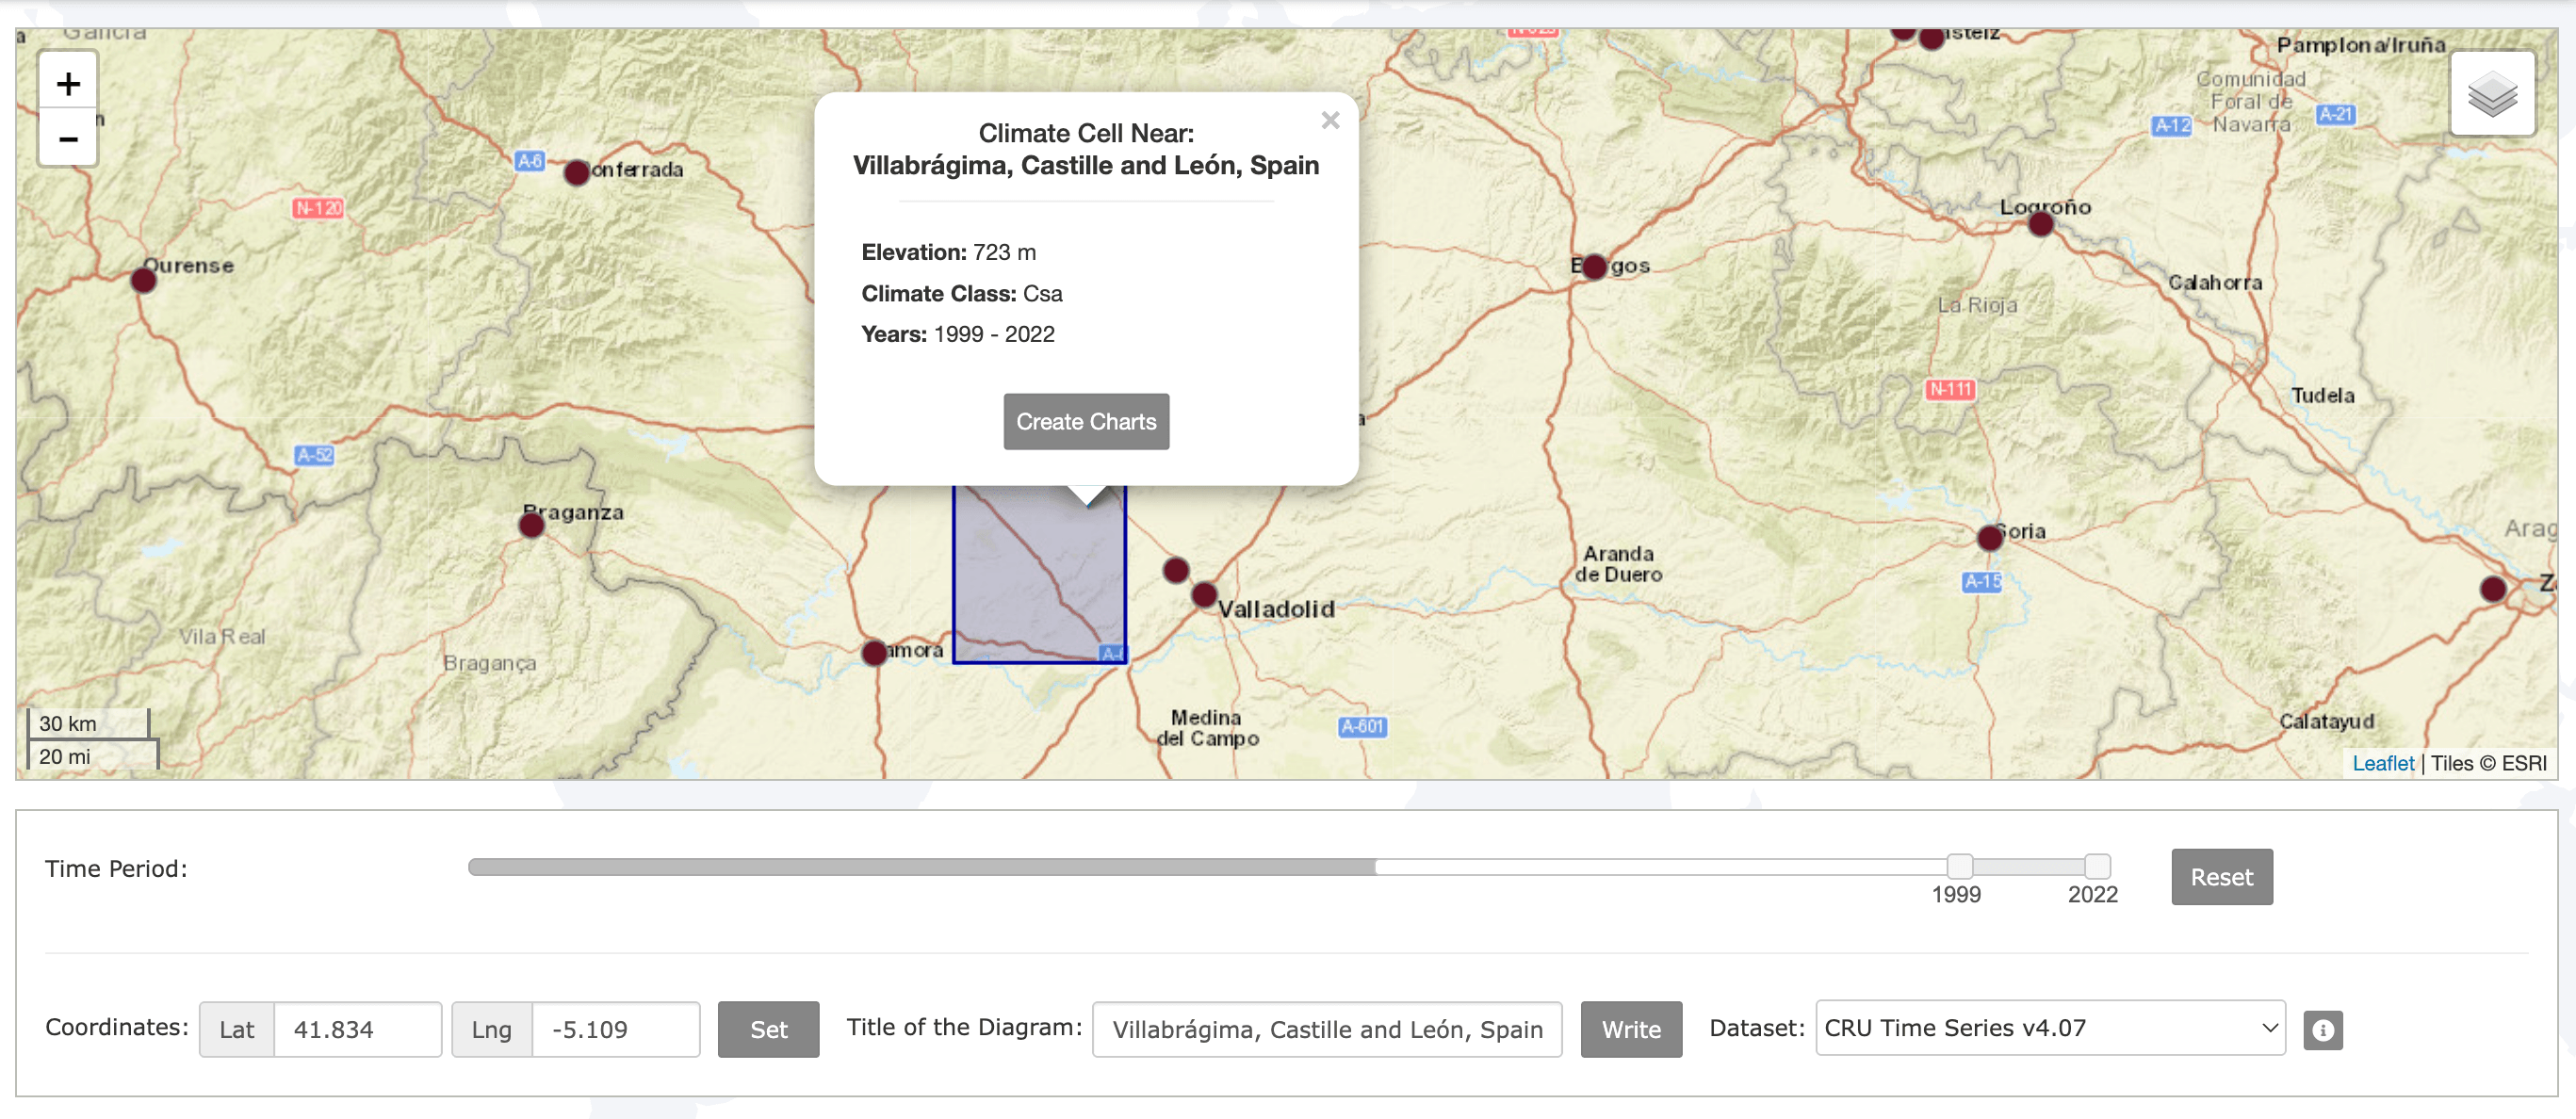
\includegraphics[width=0.9\textwidth]{Images/climatecharts-map.png}
  }
  \subfigure[Resulting Walter-Lieth climatogram with monthly data table.]{
    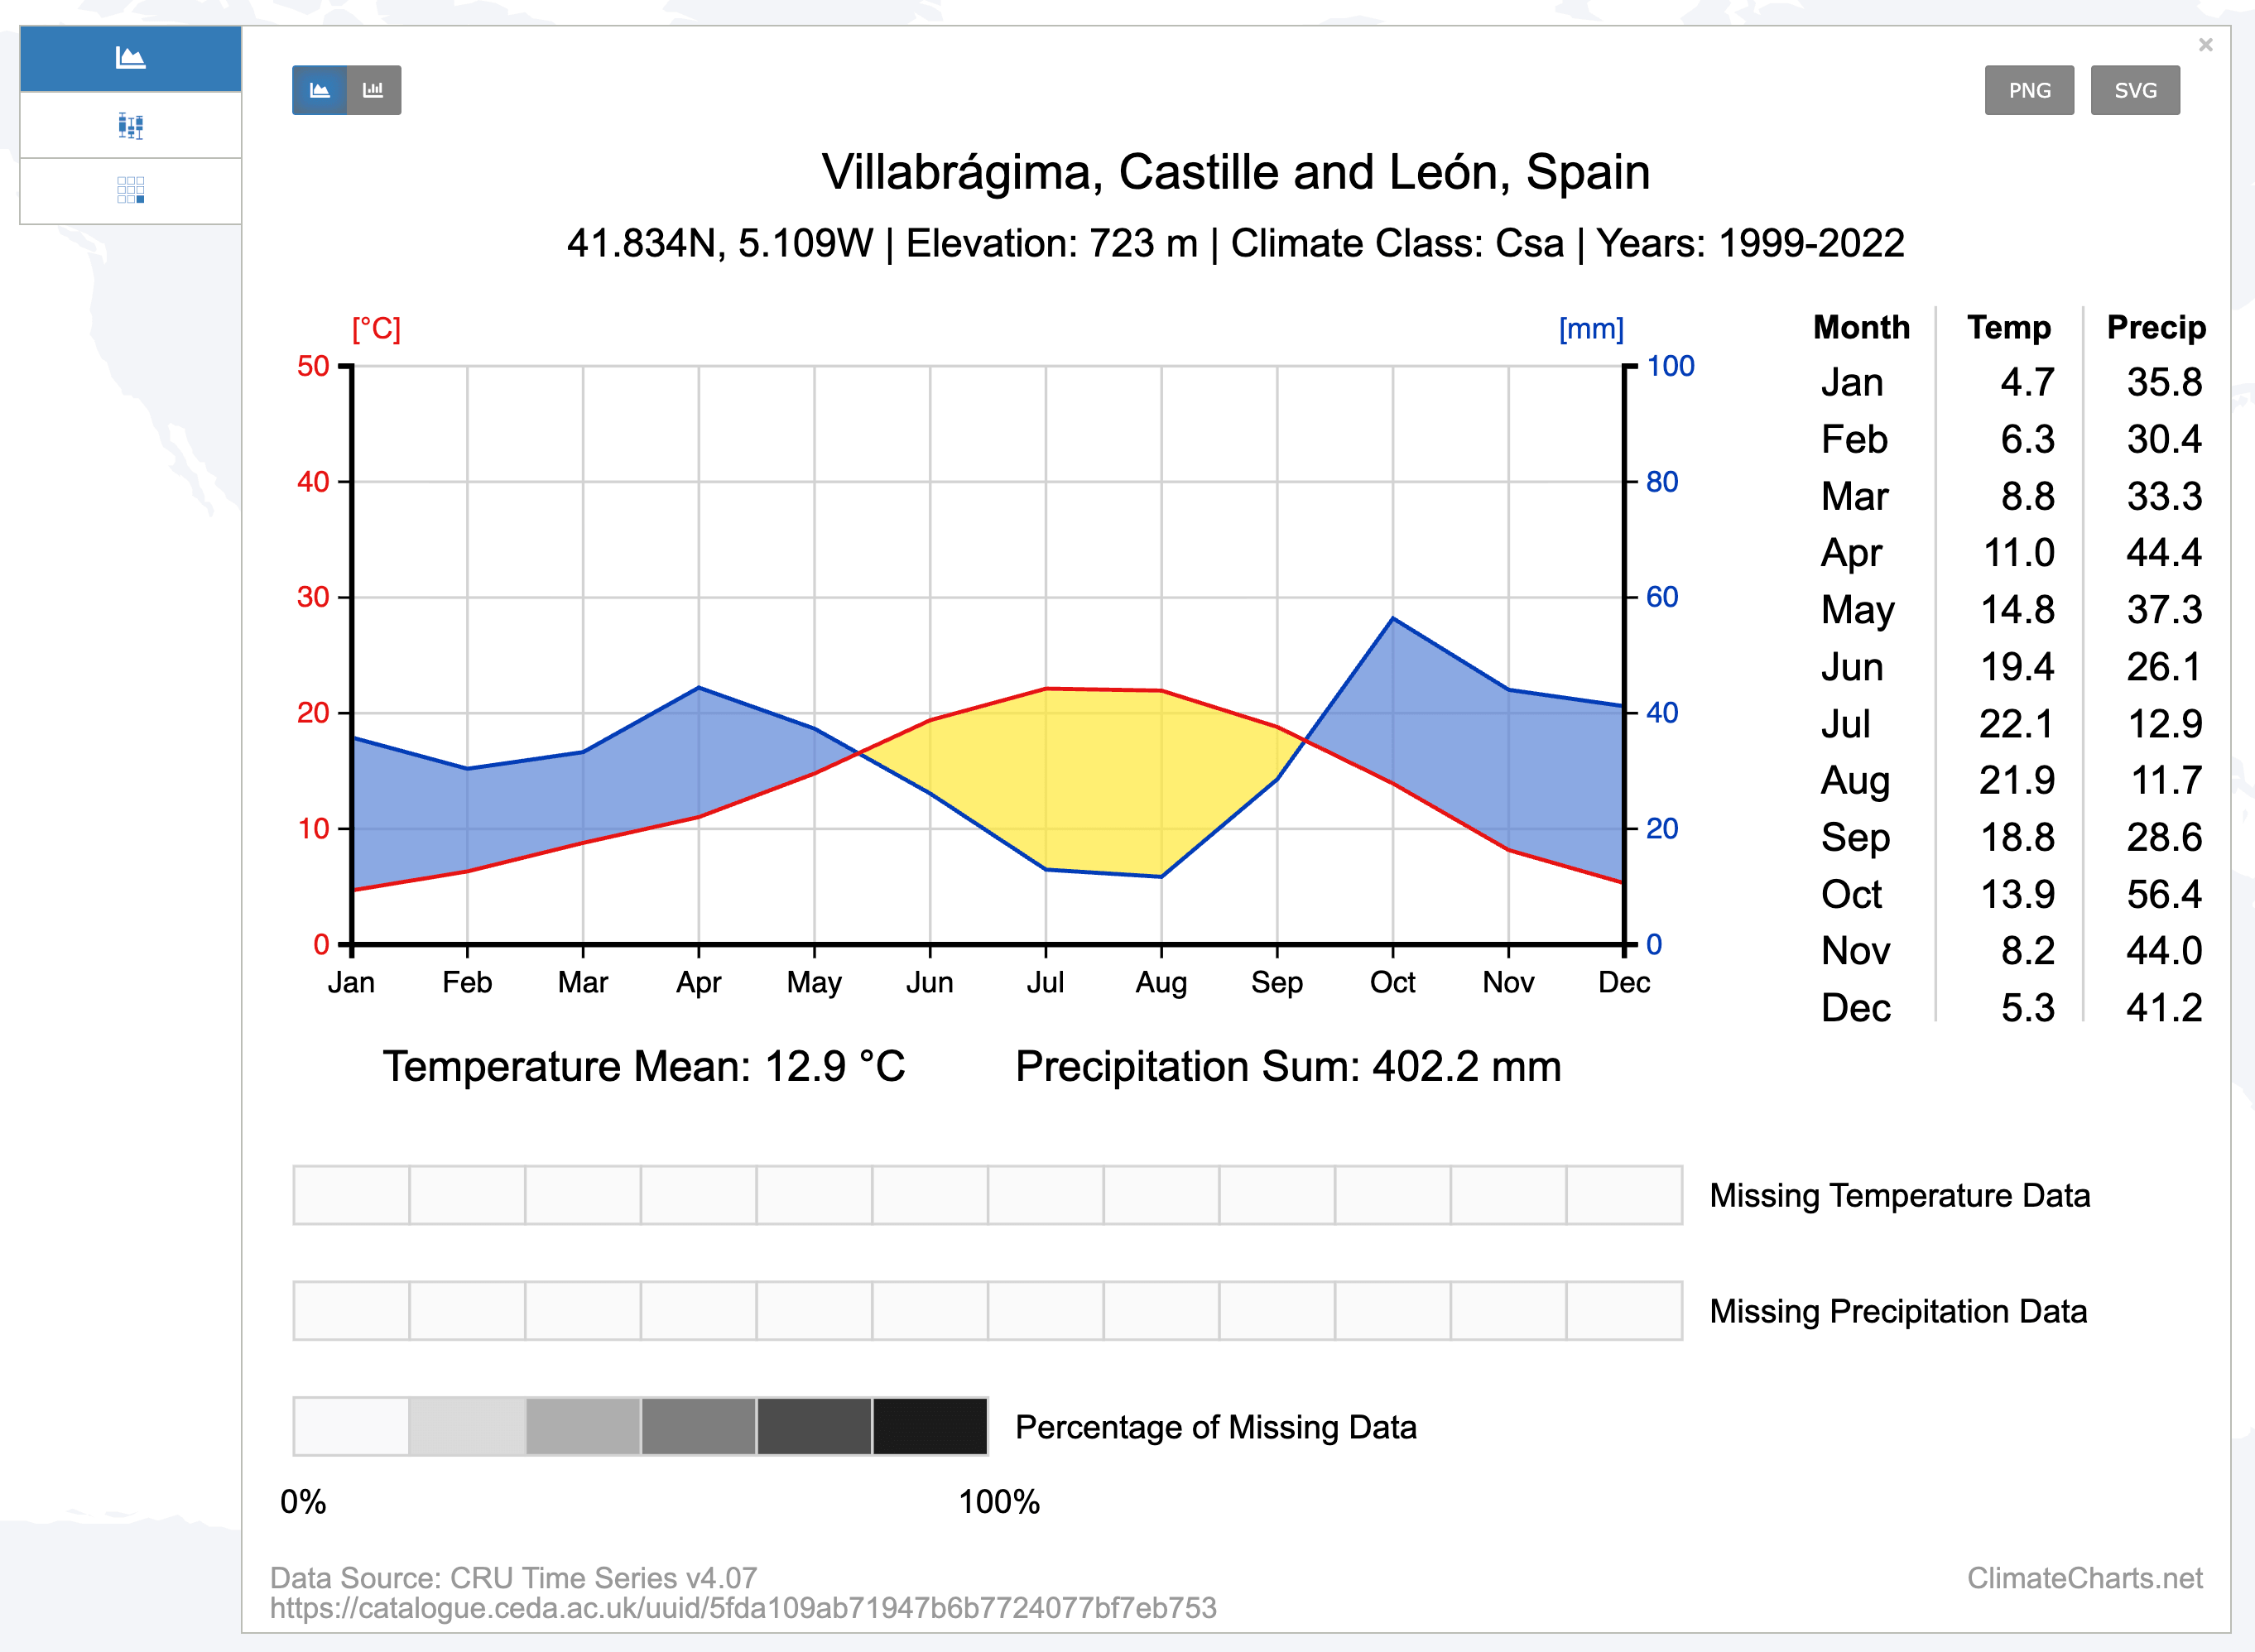
\includegraphics[width=0.9\textwidth]{Images/climatecharts-chart.png}
  }
  \caption{Climate-Charts.net interface. The tool produces clean Walter-Lieth
    climatograms but is limited to a single location view with no comparison or
    temporal exploration features.}
  \label{fig:screenshot_climatecharts}
\end{figure}

Climatica draws direct inspiration from the climatogram concept used by this
tool, but extends it with multi-city comparison, period comparison, and regional
heatmap views, all backed by the kilometre-scale raster archive of WorldClim
rather than sparse station data.

\subsection{Climate-Data.org}\label{REL_APPS_CLIMATEDATA}

Climate-Data.org~\cite{climatedataorg} provides climate statistics and
climatograms for thousands of cities worldwide. Each city page displays monthly
averages for temperature and precipitation alongside a pre-rendered diagram.
The site is primarily informational: data are presented as static charts and
tables with no interactive controls beyond city selection.

From a user-experience perspective, the interface can feel cluttered, with
advertising banners and navigation menus that are not immediately intuitive for
a first-time visitor. The data themselves are reliable --- the site draws on
established meteorological records --- but the presentation prioritises
comprehensiveness over clarity. A user who wants only to understand the broad
seasonal pattern of a location must scroll past a considerable amount of
supplementary content to find the chart.

The absence of comparative or temporal views means the site is not suited to
exploratory analysis. There is no way to ask questions such as ``how does the
summer in Valladolid compare to that in Kyiv?'' or ``has the dry season in this
city become longer over the past fifty years?''. The site does not expose a
public API, so its data cannot be consumed programmatically by third-party
applications.

\begin{figure}[H]
  \centering
  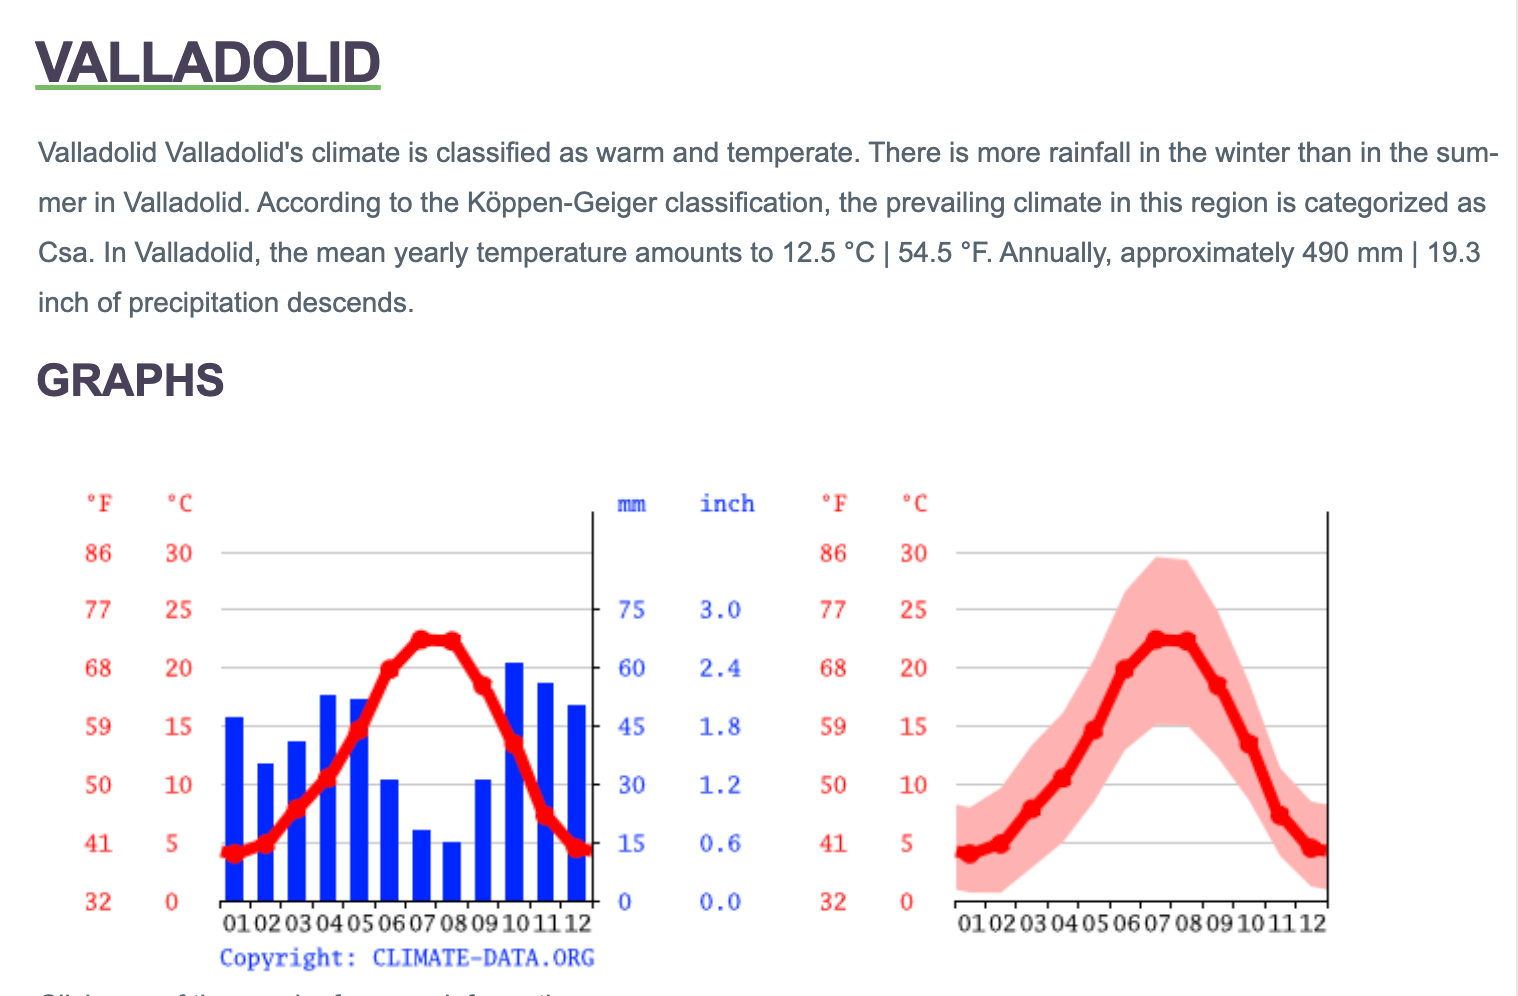
\includegraphics[width=0.9\textwidth]{Images/climatedata.png}
  \caption{Climate-Data.org city page. The static climatogram and data tables
    are embedded among advertising and navigation elements, making the interface
    feel cluttered for a user interested primarily in the chart.}
  \label{fig:screenshot_climatedata}
\end{figure}

\subsection{Meteoblue}\label{REL_APPS_METEOBLUE}

Meteoblue~\cite{meteoblue} is a commercial weather and climate platform that
offers high-resolution forecasts, historical reanalysis data, and climate
simulations. Its History and Climate module provides multi-decadal statistics
for any location, displaying average temperatures, precipitation, hot days,
cold nights, and wind speed on a single interactive chart. The platform is aimed
at a broad audience ranging from casual users planning holidays to professionals
in agriculture, aviation, and construction.

Compared to Climate-Charts.net and Climate-Data.org, Meteoblue provides
considerably more information per view: a single chart may overlay five or more
variables simultaneously, and the interface includes a Climate Comparison
feature that allows two locations to be placed side by side. In this respect,
Meteoblue overlaps with several of Climatica's objectives.

However, there are meaningful differences in scope and data source. Meteoblue
relies on ERA5T, a proprietary reanalysis model produced by ECMWF that combines
observational data with numerical weather modelling. This makes it well suited
for recent weather reconstruction but less directly comparable with the
station-interpolated WorldClim surfaces that Climatica uses. Furthermore, the
density of information presented --- multiple overlapping lines, dual axes, and
a legend with five entries --- can be overwhelming for a first-time user who
simply wants to know whether July is dry or wet in a given city. Climatica takes
a different design choice: fewer variables per view, a cleaner visual hierarchy,
and a focus on the Walter-Lieth convention that many geography students and
educators already know.

\begin{figure}[H]
  \centering
  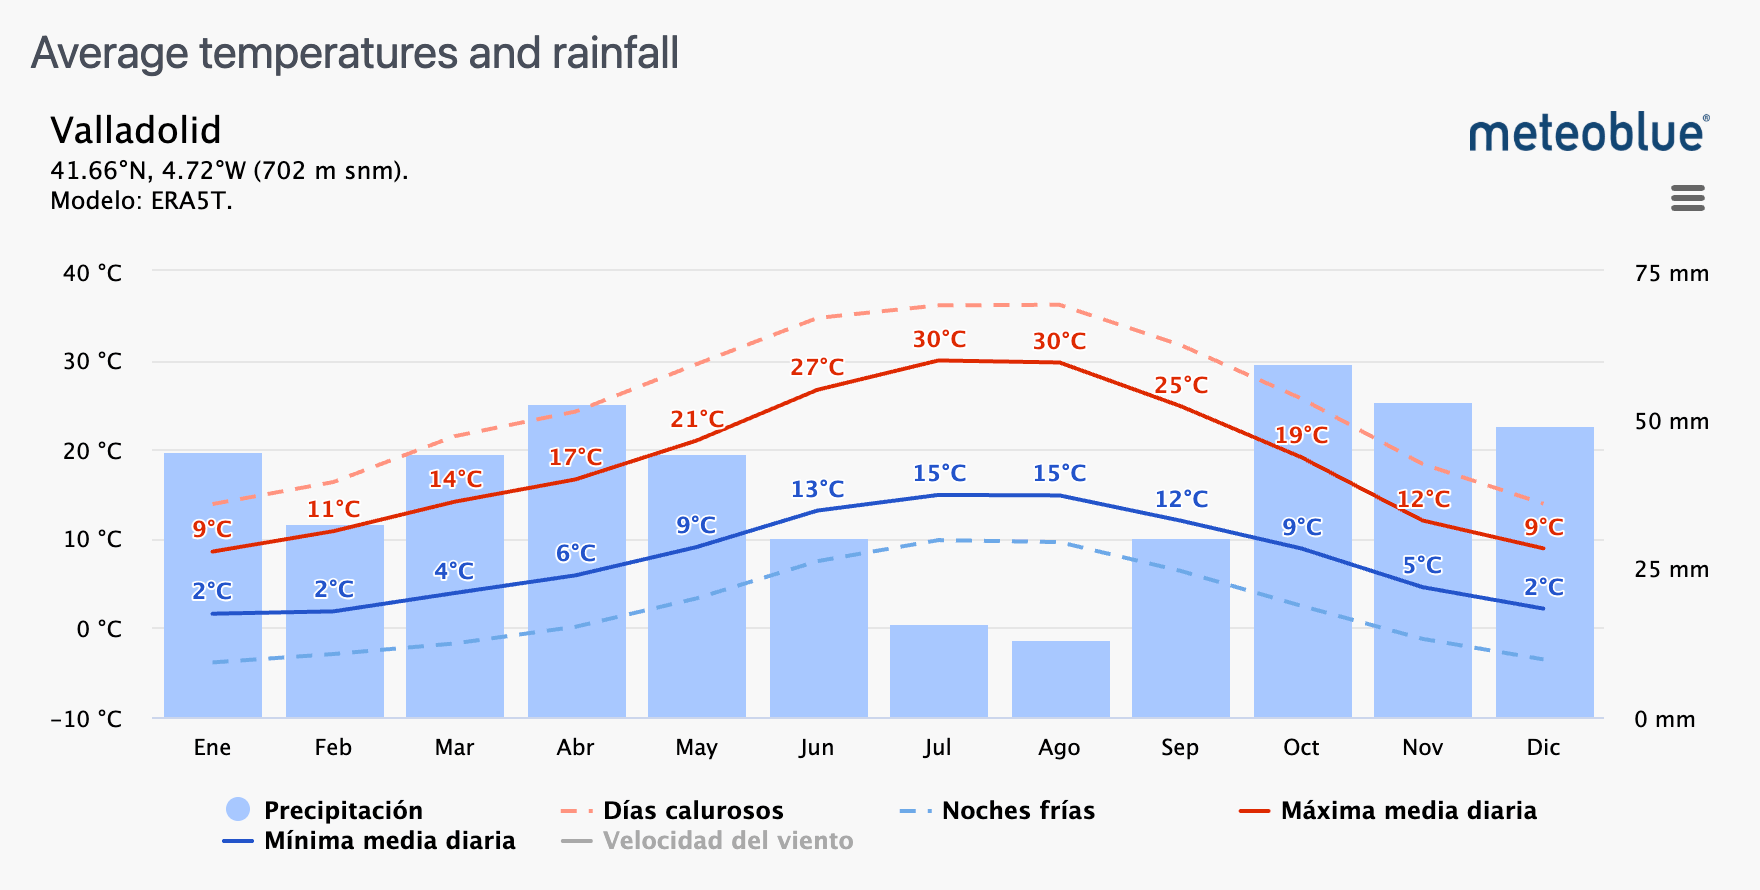
\includegraphics[width=0.9\textwidth]{Images/meteoblue.png}
  \caption{Meteoblue History and Climate module for Valladolid. The chart
    overlays five climate variables simultaneously and is backed by the ERA5T
    reanalysis model. The platform offers more data per view than
    Climate-Charts.net but targets a different audience and data source than
    Climatica.}
  \label{fig:screenshot_meteoblue}
\end{figure}

\subsection{Köppen-Geiger Climate Classification Maps}\label{REL_APPS_KOPPEN}

Several web tools visualise the Köppen-Geiger climate classification system,
which partitions the Earth's surface into climate zones based on long-term
temperature and precipitation thresholds~\cite{koppen}. These tools typically
render a world map with colour-coded zones and allow the user to click on a
location to read its classification. The most widely used online version is
based on the updated global map by Beck et al.~\cite{beck2018koppen}, which
uses the WorldClim dataset as its primary data source.

While geographically comprehensive and visually compelling, Köppen-Geiger
viewers are essentially static: they communicate a single derived variable (the
climate class) and offer no access to the underlying monthly values from which
that class was computed. A user can learn that Valladolid has a \emph{BSk}
(cold semi-arid) climate, but cannot inspect the monthly temperature curve or
compare the precipitation totals of different years. They are closer to
reference posters than to data exploration tools.

\subsection{NASA Giovanni}\label{REL_APPS_GIOVANNI}

NASA Giovanni~\cite{giovanni} (Geospatial Interactive Online Visualization ANd
aNalysis Infrastructure) is a web-based platform developed by NASA's Goddard
Earth Sciences Data and Information Services Center (GES DISC). It provides
access to a vast archive of satellite-derived geophysical data, including
surface temperature, precipitation, aerosol optical depth, and dozens of other
atmospheric and land-surface variables. The platform is designed for scientific
research and supports a wide range of analysis operations: time-series
extraction, area-averaged plots, spatial maps, correlation analyses, and
hovmöller diagrams, among others.

Giovanni's primary strength is the breadth and scientific rigour of its data
holdings. Variables are derived from well-validated satellite missions such as
MODIS, TRMM, and GPM, and the platform provides access to data spanning
multiple decades. The spatial coverage is global, and the temporal resolution
ranges from daily to monthly depending on the variable and mission.

However, Giovanni is clearly designed for atmospheric scientists and remote
sensing specialists. The workflow for retrieving data requires the user to
navigate a multi-step interface: select a variable from a hierarchical catalogue
of thousands of datasets, specify a spatial bounding box, choose a time range,
select an analysis type, and submit a processing job that may take several
minutes to complete. The results are returned as downloadable files or rendered
charts, but there is no interactive exploration mode in which a user can click a
city on a map and immediately see its climate profile. The platform is powerful
but has a steep learning curve that puts it out of reach for non-specialist
users.

\begin{figure}[H]
  \centering
  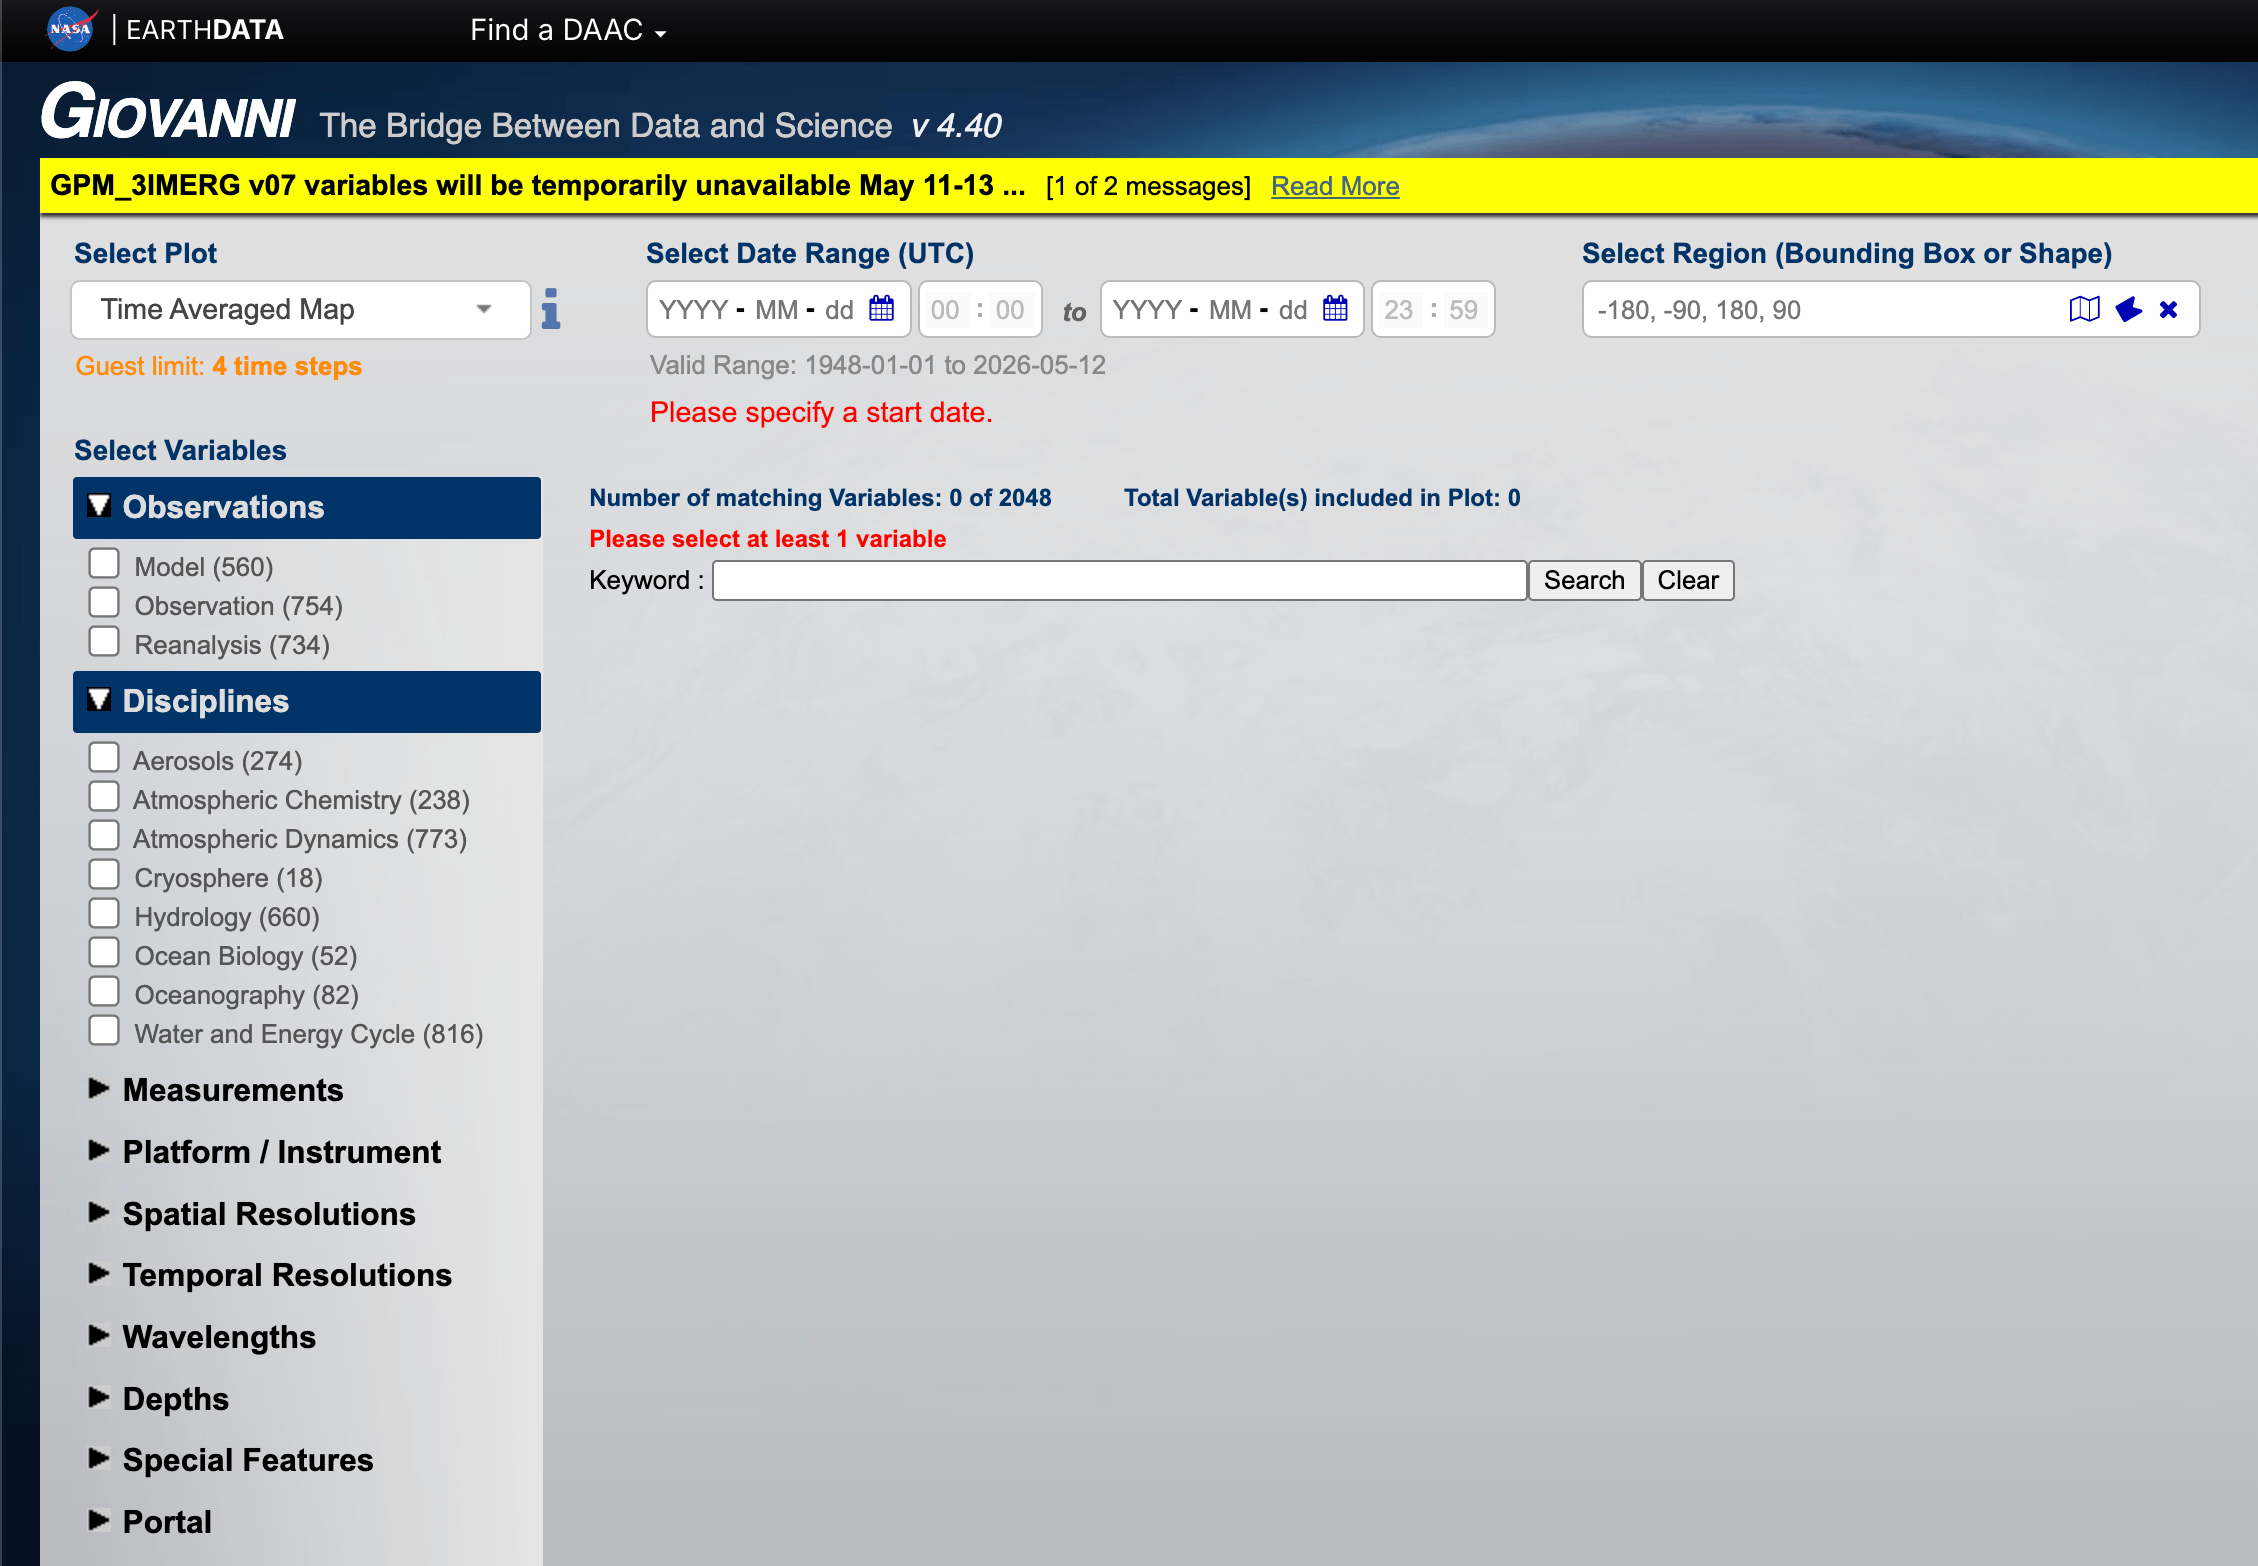
\includegraphics[width=0.9\textwidth]{Images/giovanni.png}
  \caption{NASA Giovanni main interface. Before any data can be retrieved, the
    user must select a plot type, specify a date range, a bounding box, and
    choose from a catalogue of 2{,}048 variables grouped by discipline. The
    empty results panel illustrates why the platform is inaccessible to
    non-specialist users.}
  \label{fig:screenshot_giovanni}
\end{figure}

\subsection{Copernicus Climate Change Service}\label{REL_APPS_COPERNICUS}

The Copernicus Climate Change Service (C3S)~\cite{copernicus}, operated by the
European Centre for Medium-Range Weather Forecasts (ECMWF) on behalf of the
European Commission, is the most comprehensive open climate data infrastructure
currently available. Its Climate Data Store (CDS) provides access to terabytes
of reanalysis data (ERA5), seasonal forecasts, climate projections, and sectoral
climate indicators, all under an open licence.

The CDS toolbox allows users to write Python scripts that retrieve, process, and
visualise data from the store, and a graphical interface is provided for simpler
operations. For users willing to engage with the toolbox, the analytical
possibilities are essentially unlimited: custom time periods, arbitrary spatial
domains, user-defined aggregations, and integration with third-party Python
libraries.

Despite this power, the C3S platform shares with NASA Giovanni the fundamental
limitation that it is designed for expert users. Accessing ERA5 data requires
registration, understanding the CDS API, and familiarity with NetCDF file
formats and Python data science libraries. The graphical interface, while
improving, remains complex and slow for simple queries such as ``what is the
typical July temperature in Seville?''. Furthermore, C3S data are reanalysis
products derived from a combination of observations and numerical weather models,
not the station-interpolated surfaces of WorldClim, so they are suited to
different use cases.

\begin{figure}[H]
  \centering
  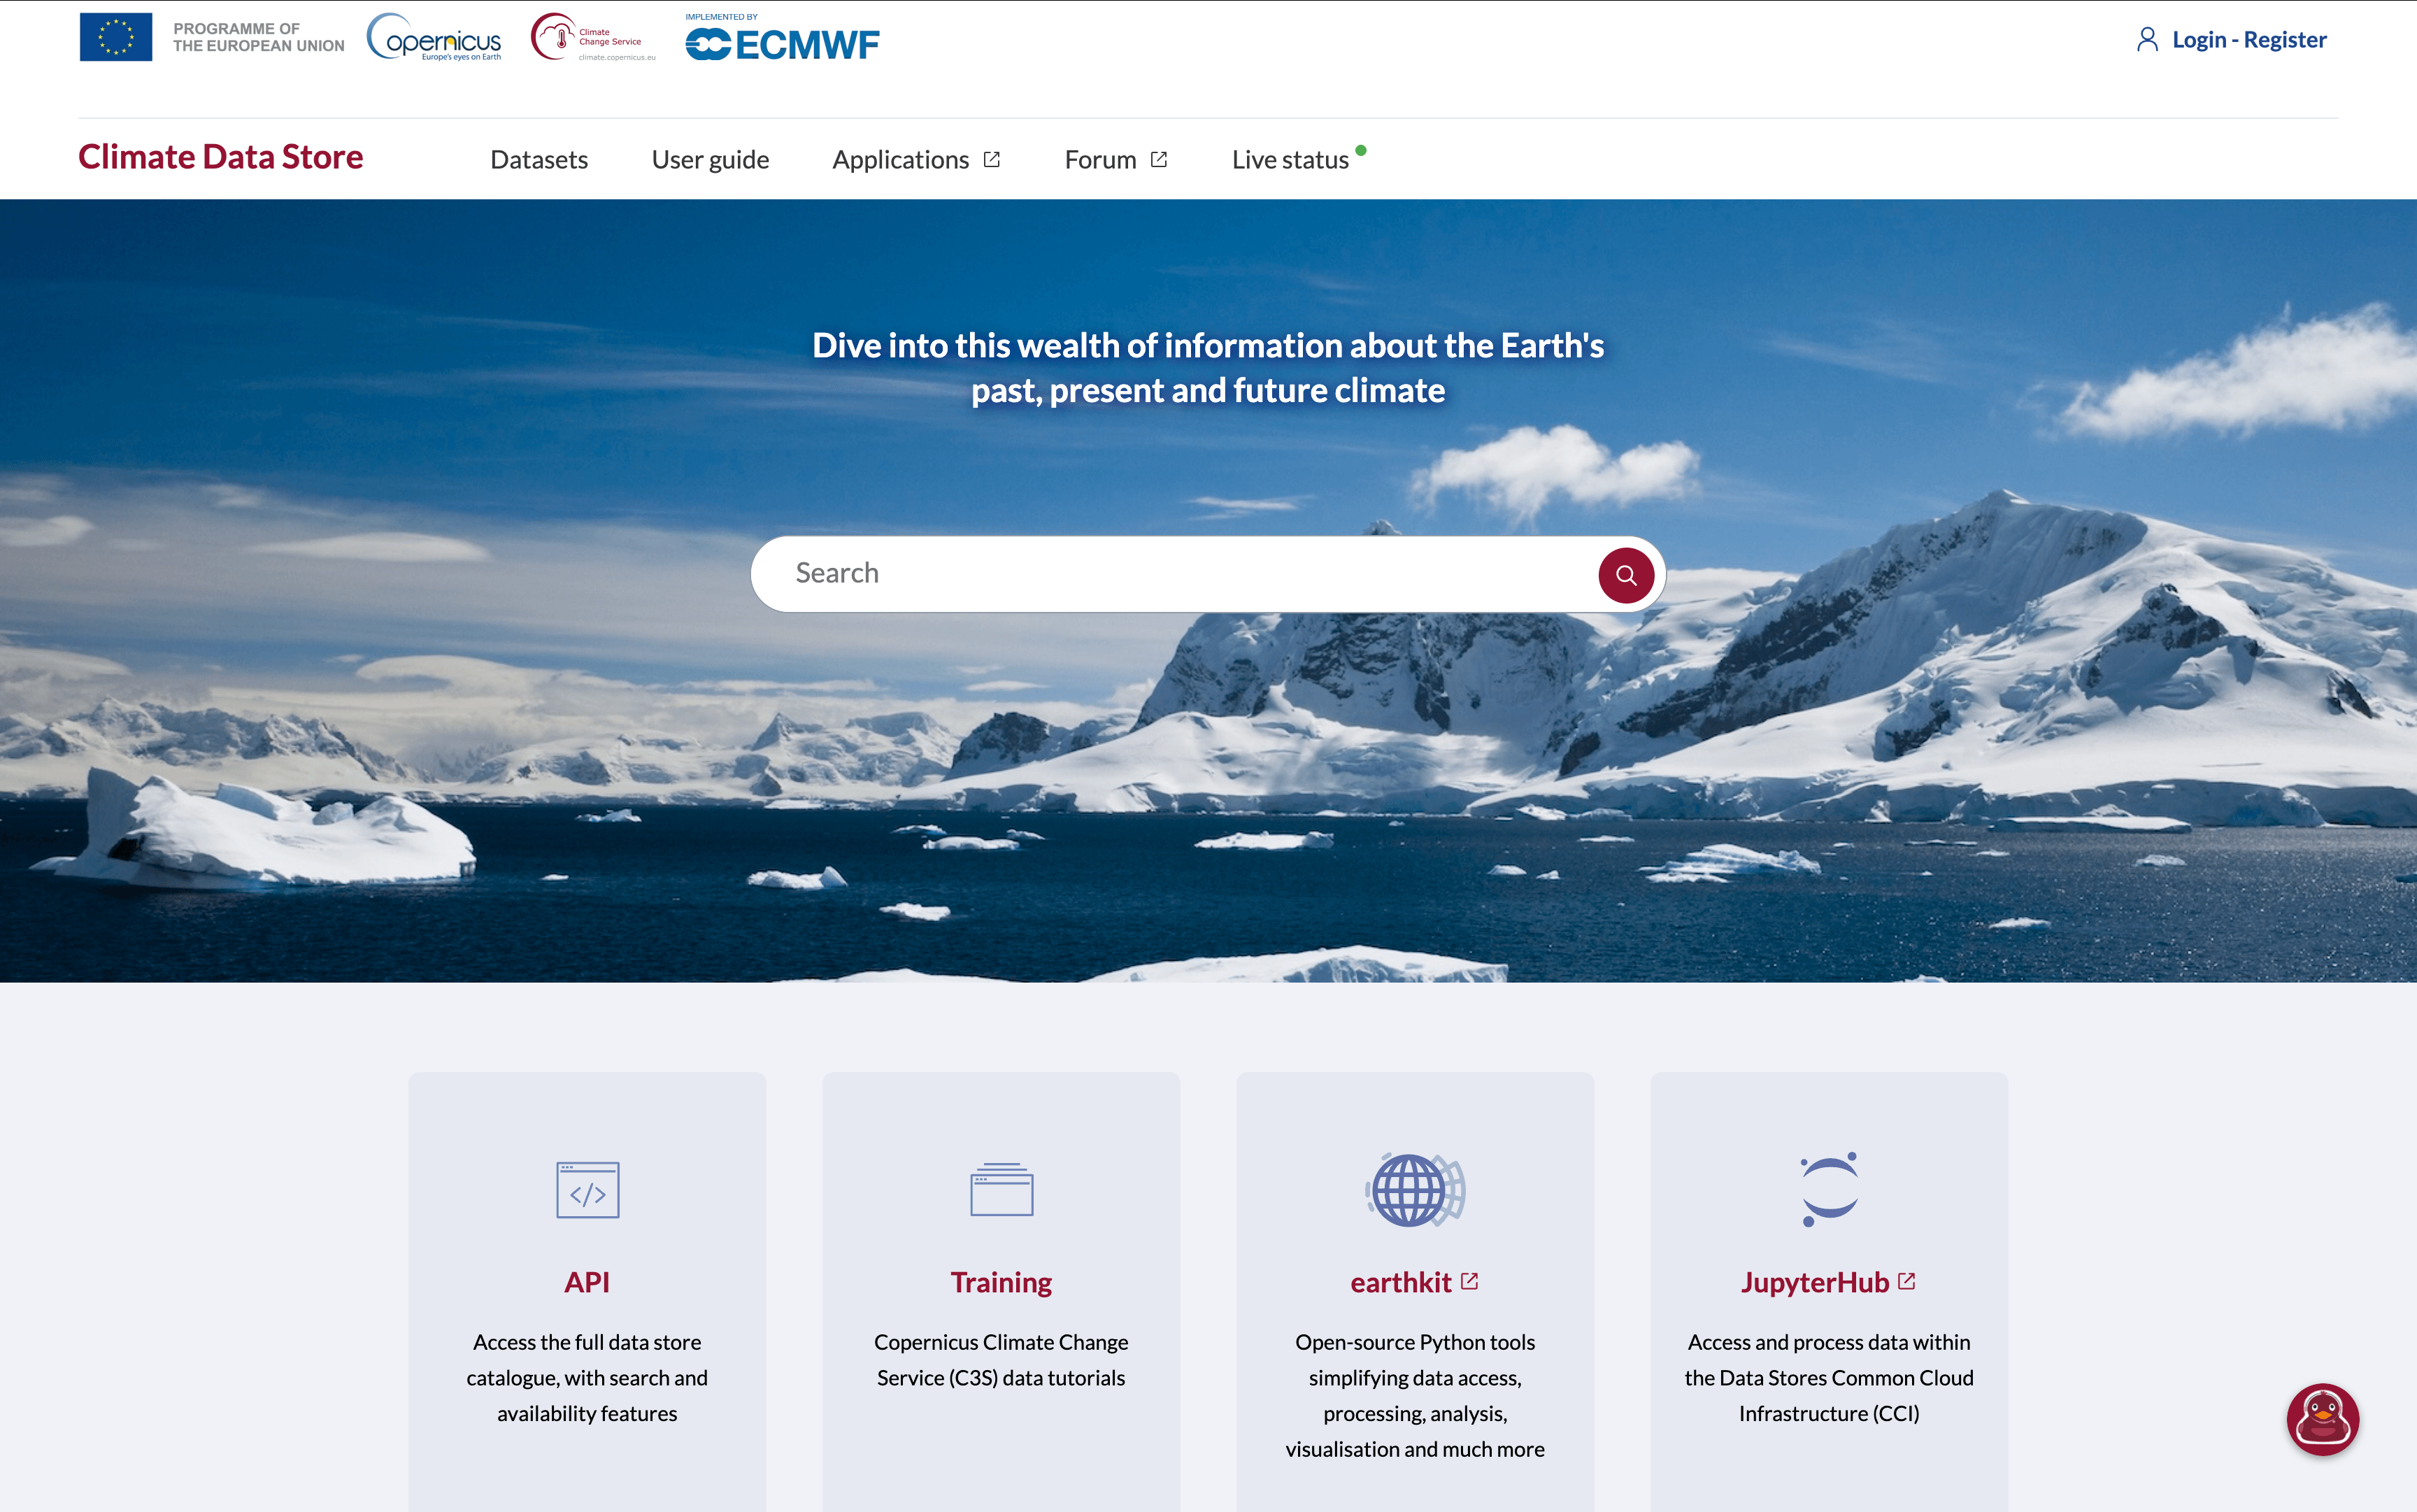
\includegraphics[width=0.9\textwidth]{Images/copernicus.png}
  \caption{Copernicus Climate Data Store landing page. The search-first
    interface and the \emph{Login~/ Register} button in the top-right corner
    illustrate that meaningful access requires both registration and prior
    knowledge of what datasets are available.}
  \label{fig:screenshot_copernicus}
\end{figure}

\subsection{Summary and Positioning of Climatica}\label{REL_APPS_SUMMARY}

Table~\ref{tab:tools} summarises the capabilities of the tools reviewed above
alongside Climatica. The comparison highlights that no existing tool combines
all of the following in a single, registration-free browser interface: open
kilometre-scale raster data, a Walter-Lieth climatogram, multi-city comparison,
period-based trend exploration, and a regional spatial heatmap.

The two most powerful platforms --- NASA Giovanni and Copernicus C3S --- offer
far greater scientific depth than Climatica, but at the cost of a steep learning
curve that excludes non-specialist users. The simpler tools --- Climate-Charts.net
and Climate-Data.org --- are accessible but static, offering a single view with
no comparative or temporal dimension. Meteoblue occupies a middle ground but
relies on proprietary data and targets professional users. Climatica is the only
tool in this survey that combines ease of use with interactive multi-view
exploration of open, globally consistent raster data.

% --- Climatica screenshots split into two figures to fit the page ---
\begin{figure}[H]
  \centering
  \subfigure[Map view with location pin, raster cell outline, and summary stat
    cards.]{
    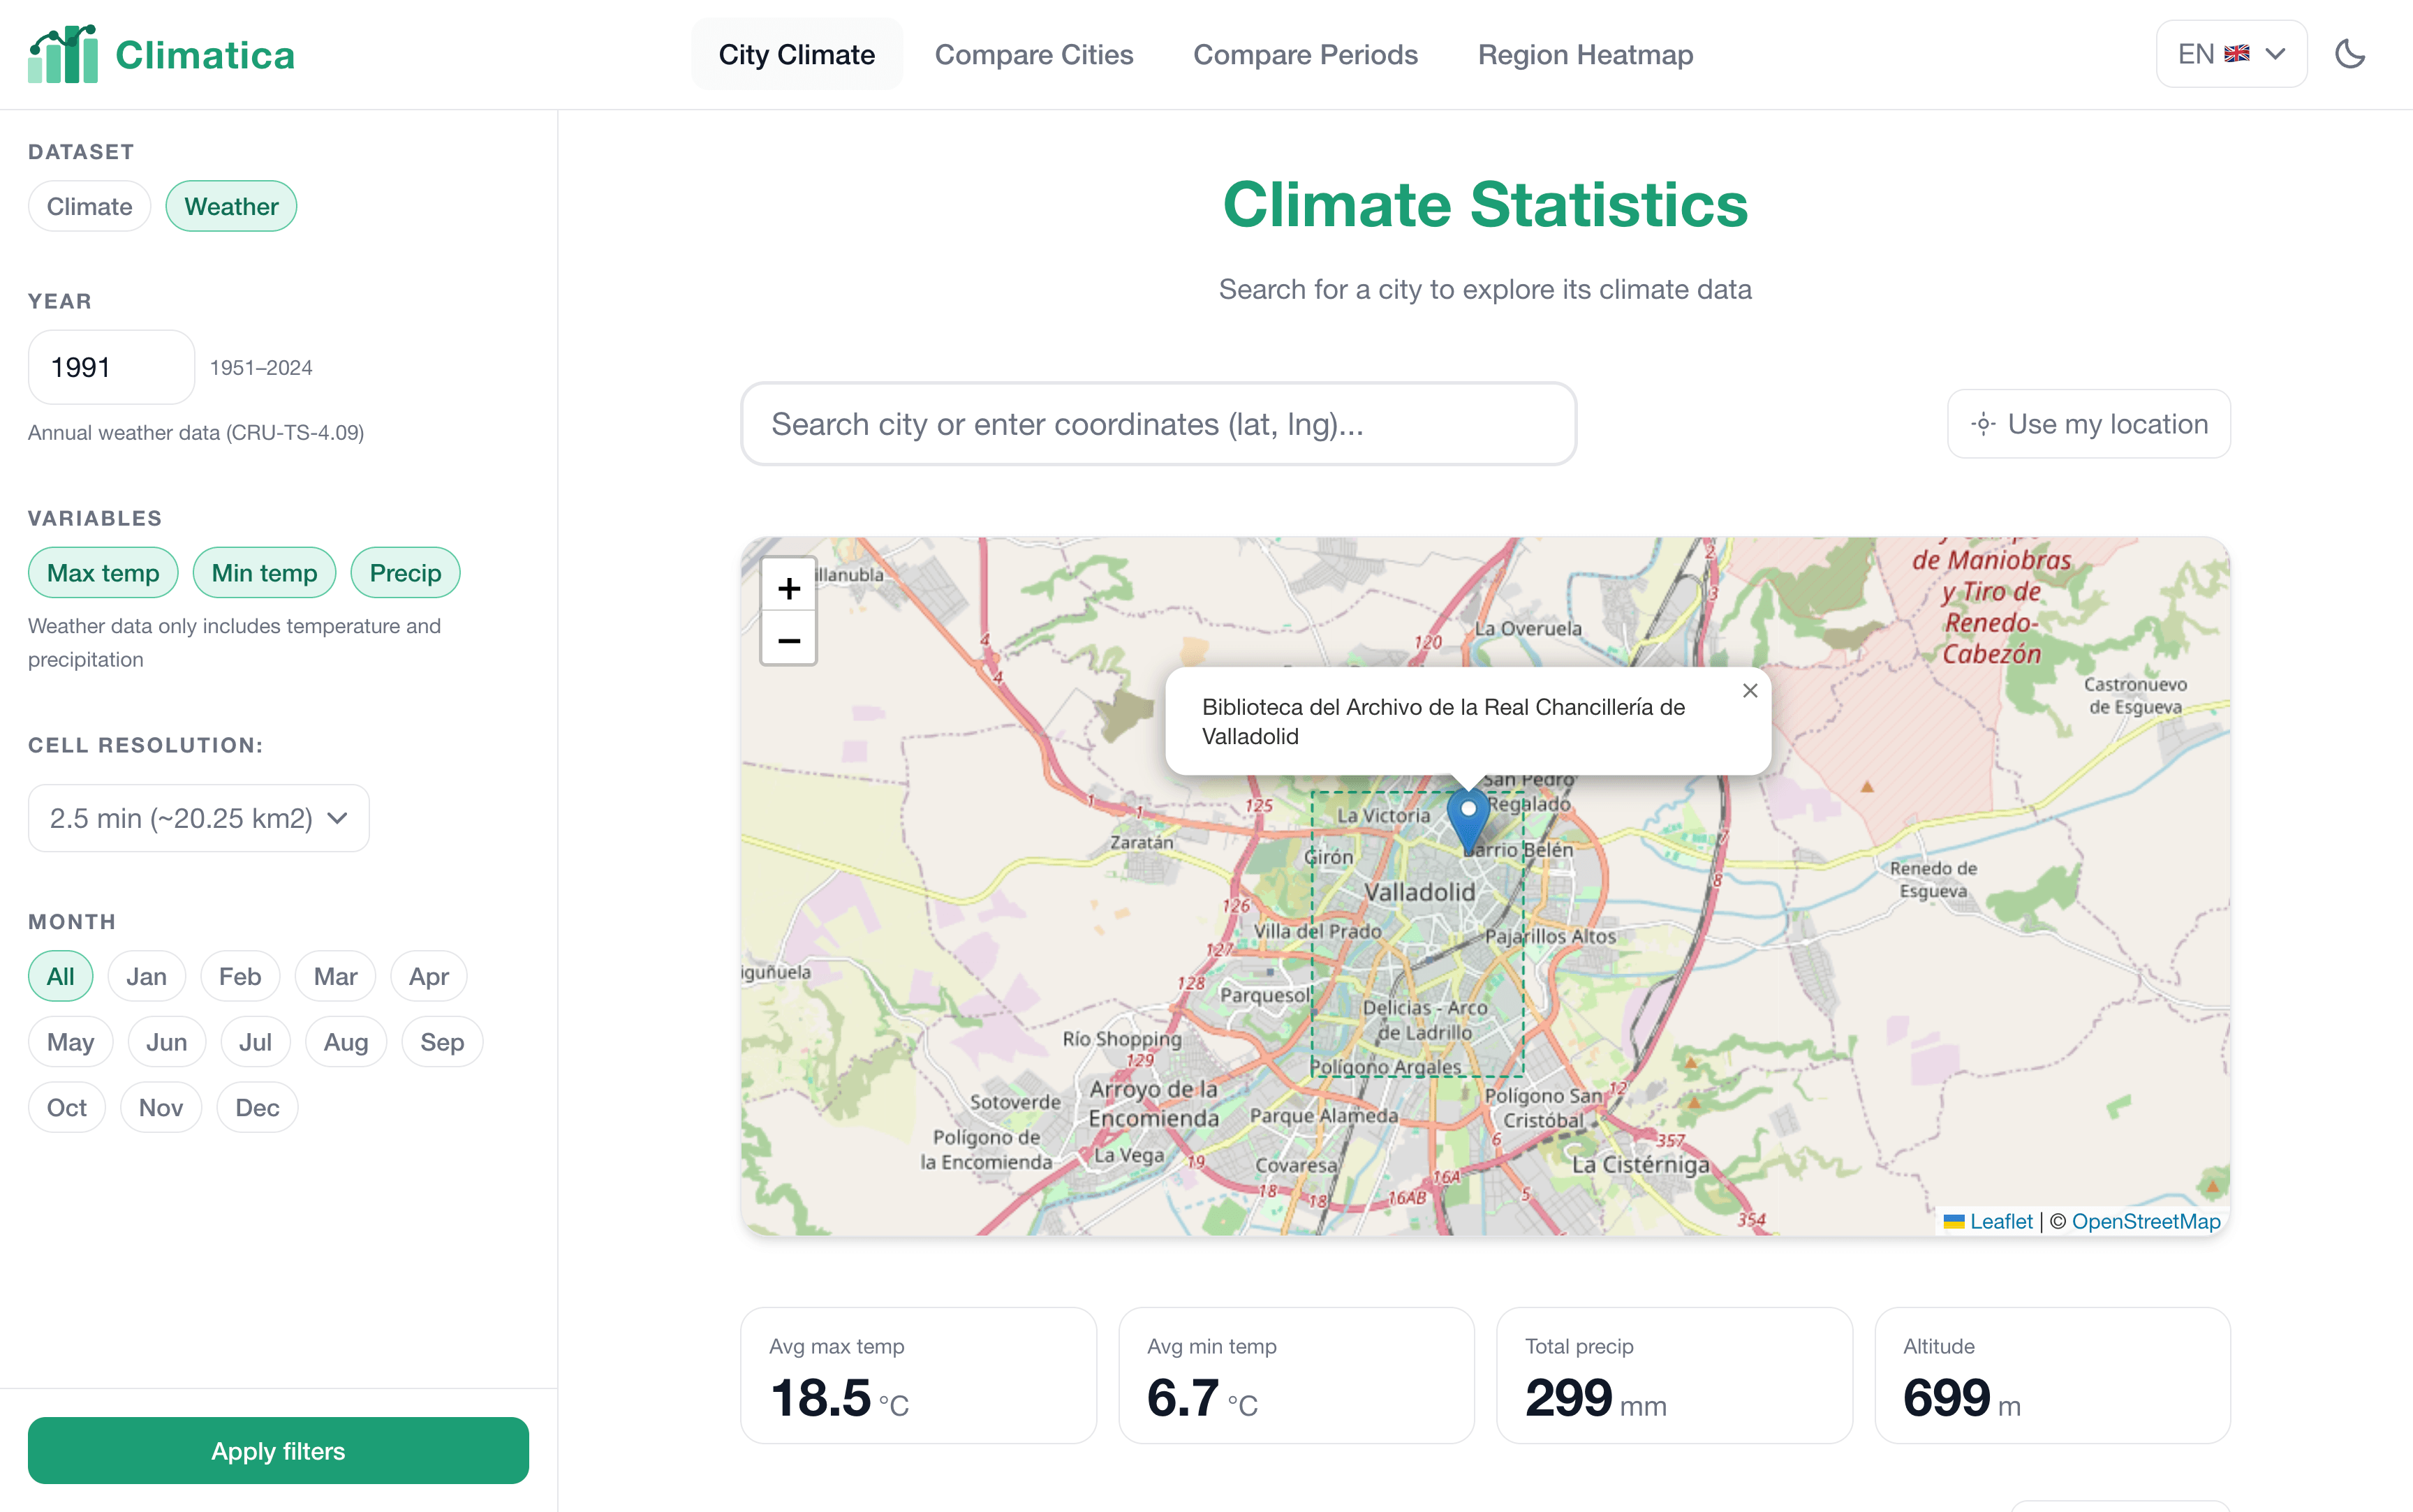
\includegraphics[width=0.9\textwidth]{Images/climatica-map.png}
  }
  \subfigure[Standard climograph: precipitation bars (blue/yellow) and
    temperature lines for the selected city.]{
    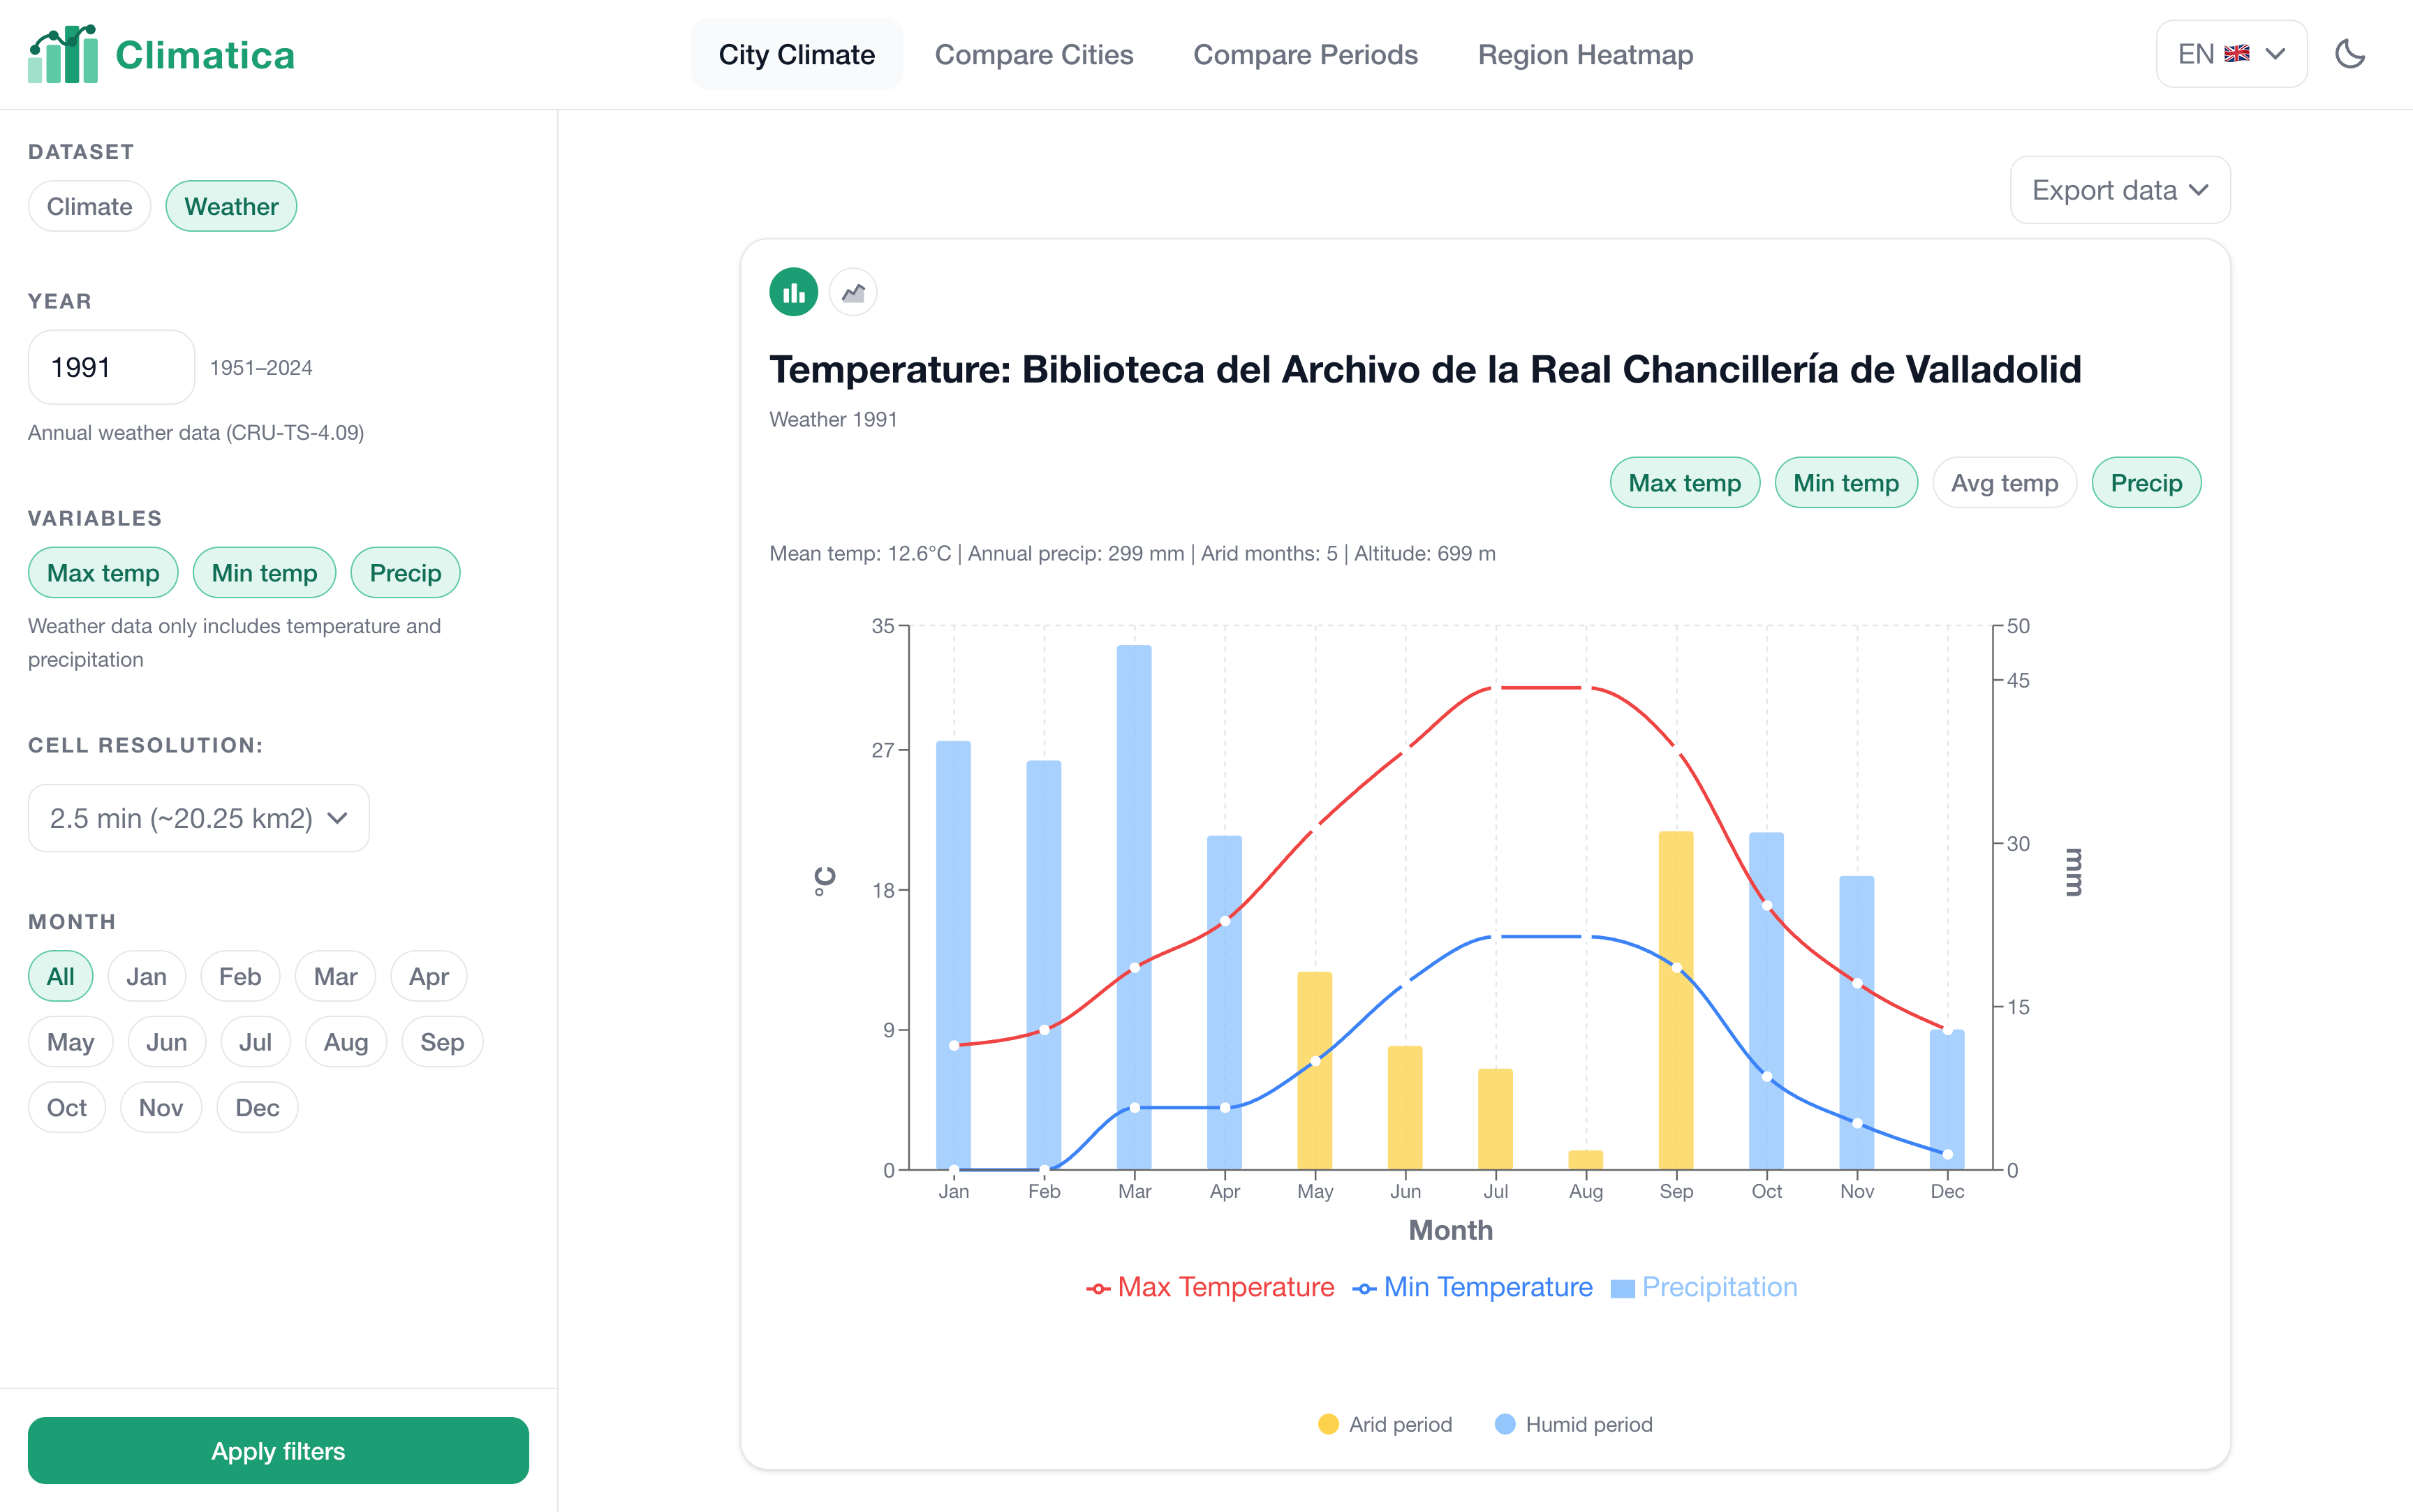
\includegraphics[width=0.9\textwidth]{Images/climatica-columns-graph.png}
  }
  \caption{Climatica City Climate page for Valladolid (weather dataset, year
    1991) --- map and standard climograph views.}
  \label{fig:screenshot_climatica_a}
\end{figure}

\begin{figure}[H]
  \centering
  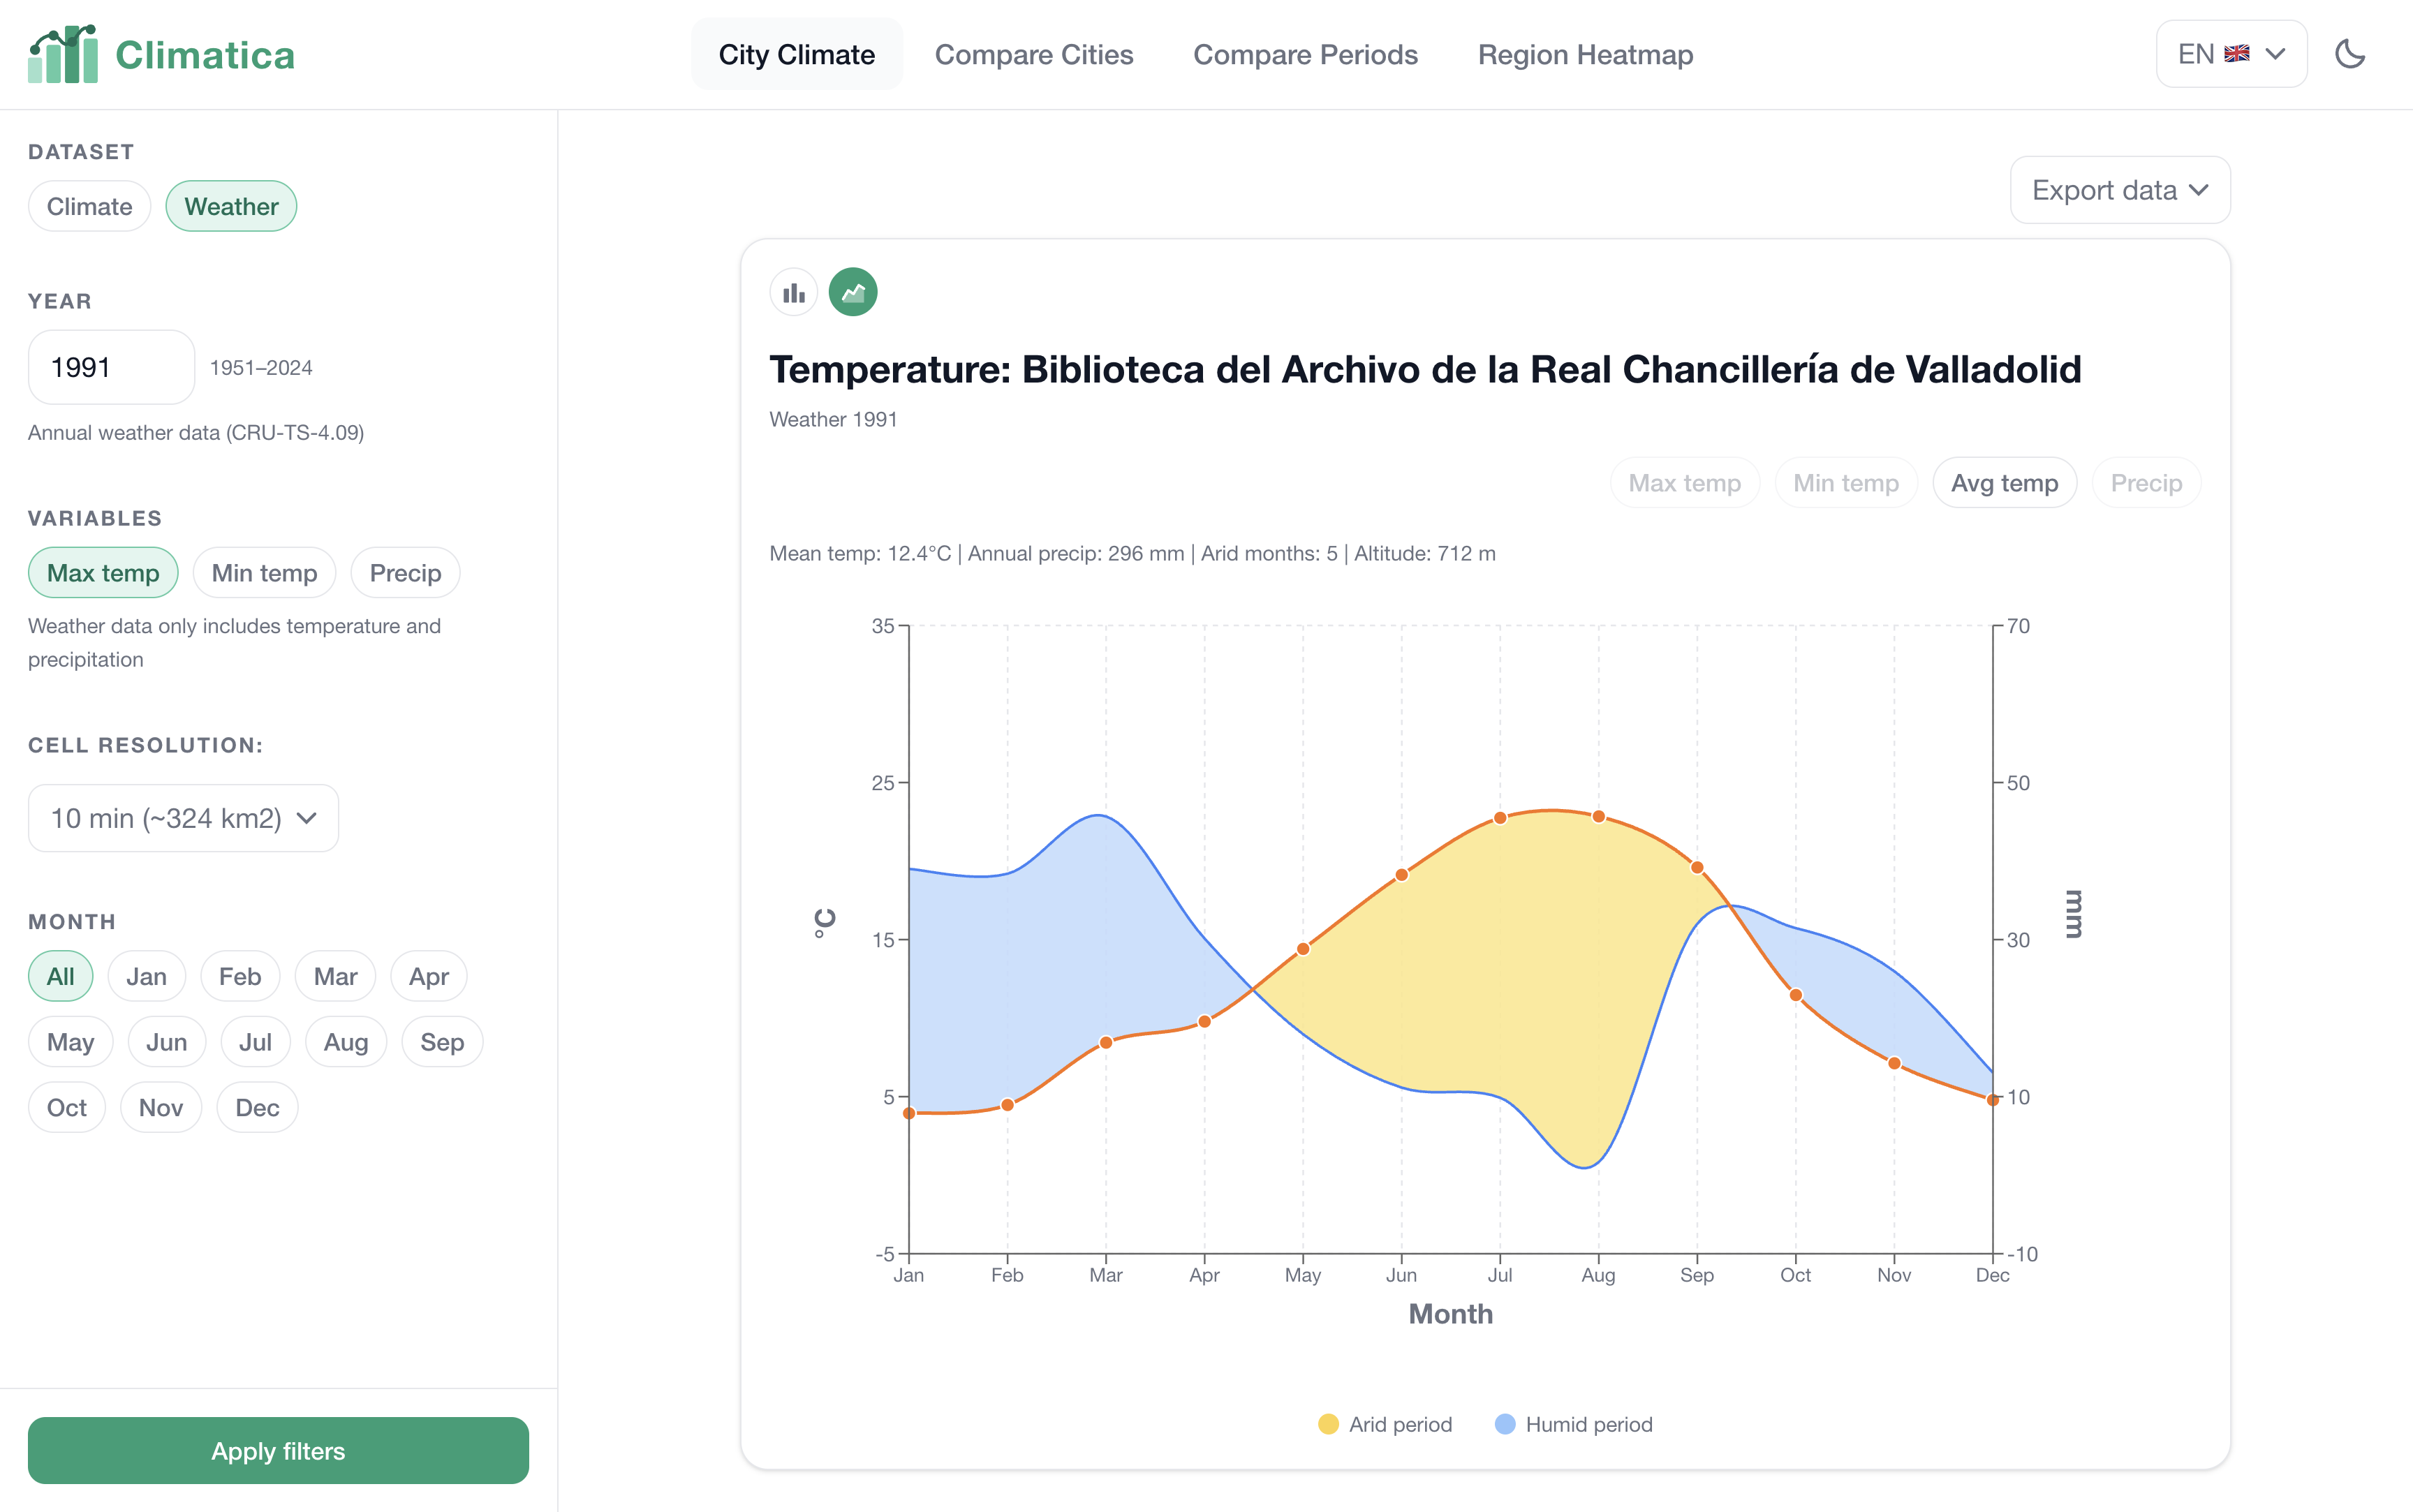
\includegraphics[width=0.9\textwidth]{Images/climatica-walter-lieth.png}
  \caption{Climatica City Climate page --- Walter-Lieth climatogram for the
    same city and period. Yellow areas indicate arid months (summer); blue areas
    indicate humid months (winter and spring). The chart uses SVG
    \texttt{clipPath} with the even-odd winding rule to produce exact arid/humid
    fills without computing curve intersection points explicitly.}
  \label{fig:screenshot_climatica_b}
\end{figure}

\begin{table}[H]
  \centering
  \caption{Comparison of climate data tools.
           \cmark~=~supported, \pmark~=~partial, \xmark~=~not supported.}
  \label{tab:tools}
  \small
  \begin{tabular}{lcccccc}
    \toprule
    \textbf{Feature} &
    \textbf{\shortstack{Climate\\Charts}} &
    \textbf{\shortstack{Climate\\Data.org}} &
    \textbf{Meteoblue} &
    \textbf{\shortstack{NASA\\Giovanni}} &
    \textbf{\shortstack{Copernicus\\C3S}} &
    \textbf{Climatica} \\
    \midrule
    City climate profile      & \cmark & \cmark & \cmark  & \xmark & \xmark & \cmark \\
    Walter-Lieth climatogram  & \cmark & \cmark & \xmark  & \xmark & \xmark & \cmark \\
    Multi-city comparison     & \xmark & \xmark & \pmark  & \xmark & \xmark & \cmark \\
    Period trend comparison   & \xmark & \xmark & \pmark  & \cmark & \cmark & \cmark \\
    Regional spatial heatmap  & \xmark & \xmark & \xmark  & \cmark & \cmark & \cmark \\
    Open km-scale data        & \xmark & \xmark & \xmark  & \cmark & \cmark & \cmark \\
    No registration required  & \cmark & \cmark & \pmark  & \xmark & \xmark & \cmark \\
    Non-specialist audience   & \cmark & \cmark & \xmark  & \xmark & \xmark & \cmark \\
    \bottomrule
  \end{tabular}
  \normalsize
\end{table}

\section{WorldClim}\label{REL_WORLDCLIM}

\subsection{The Dataset}\label{REL_WORLDCLIM_DATA}

WorldClim is a global database of high-resolution climate data widely used in
ecology, biogeography, agriculture, and climate-change research. Version~2.1,
described by Fick and Hijmans~\cite{fick2017worldclim}, provides interpolated
monthly climate surfaces derived from weather-station observations collected
between 1970 and 2000. The dataset covers the entire land surface of the Earth
at four spatial resolutions: 10 arc-minutes ($\approx$18.5\,km at the equator),
5 arc-minutes ($\approx$9.2\,km), 2.5 arc-minutes ($\approx$4.6\,km), and 30
arc-seconds ($\approx$900\,m).

Seven monthly variables are available in the climate dataset: minimum temperature
(\texttt{tmin}), maximum temperature (\texttt{tmax}), average temperature
(\texttt{tavg}), precipitation (\texttt{prec}), solar radiation (\texttt{srad}),
wind speed (\texttt{wind}), and vapour pressure (\texttt{vapr}). Climatica uses
\texttt{tmin}, \texttt{tmax}, \texttt{tavg}, and \texttt{prec} --- the four
variables most relevant to general climate characterisation and to the
construction of Walter-Lieth climatograms.

\subsubsection{Bioclimatic Variables}\label{REL_WORLDCLIM_BIO}

In addition to the seven monthly variables, WorldClim provides 19 bioclimatic
variables (BIO1--BIO19) derived algorithmically from the monthly temperature and
precipitation series. These variables were designed to capture biologically
meaningful aspects of climate that are not immediately apparent from the raw
monthly values, and they are widely used as predictors in species distribution
models and ecological niche analyses.

Table~\ref{tab:bio} lists the 19 bioclimatic variables. Several of them have
intuitive interpretations: BIO1 is simply the annual mean temperature, BIO12 is
the total annual precipitation, and BIO4 (temperature seasonality) measures how
much monthly temperatures vary across the year. Others capture more specific
relationships, such as BIO8 (mean temperature of the wettest quarter) and BIO18
(precipitation of the warmest quarter), which are particularly relevant for
understanding vegetation patterns in seasonally dry regions.

\begin{table}[H]
  \centering
  \caption{WorldClim bioclimatic variables (BIO1--BIO19).}
  \label{tab:bio}
  \begin{tabular}{ll}
    \toprule
    \textbf{Code} & \textbf{Description} \\
    \midrule
    BIO1  & Annual Mean Temperature \\
    BIO2  & Mean Diurnal Range (Mean of monthly max$-$min) \\
    BIO3  & Isothermality (BIO2/BIO7 $\times$ 100) \\
    BIO4  & Temperature Seasonality (standard deviation $\times$ 100) \\
    BIO5  & Max Temperature of Warmest Month \\
    BIO6  & Min Temperature of Coldest Month \\
    BIO7  & Temperature Annual Range (BIO5$-$BIO6) \\
    BIO8  & Mean Temperature of Wettest Quarter \\
    BIO9  & Mean Temperature of Driest Quarter \\
    BIO10 & Mean Temperature of Warmest Quarter \\
    BIO11 & Mean Temperature of Coldest Quarter \\
    BIO12 & Annual Precipitation \\
    BIO13 & Precipitation of Wettest Month \\
    BIO14 & Precipitation of Driest Month \\
    BIO15 & Precipitation Seasonality (Coefficient of Variation) \\
    BIO16 & Precipitation of Wettest Quarter \\
    BIO17 & Precipitation of Driest Quarter \\
    BIO18 & Precipitation of Warmest Quarter \\
    BIO19 & Precipitation of Coldest Quarter \\
    \bottomrule
  \end{tabular}
\end{table}

Although Climatica does not currently expose the bioclimatic variables in its
user interface --- focusing instead on the monthly temperature and precipitation
series that are more interpretable for general users --- the SCRAPI API provides
full access to them, and they represent a natural direction for future extension
of the application.

\subsubsection{Interpolation Methodology}\label{REL_WORLDCLIM_INTERP}

The WorldClim surfaces are not direct observations: they are the result of a
spatial interpolation procedure applied to records from tens of thousands of
weather stations distributed unevenly across the globe. The interpolation method
used in WorldClim~2.1 is ANUSPLIN~\cite{hutchinson1995}, a thin-plate smoothing
spline algorithm that models the relationship between a climate variable and
geographic predictors --- primarily latitude, longitude, and elevation.

Elevation plays a particularly important role because temperature decreases with
altitude at a relatively predictable rate (the environmental lapse rate), while
orographic effects strongly influence precipitation on windward and leeward
slopes. By incorporating a digital elevation model as a covariate, ANUSPLIN can
produce surfaces that reflect the local topographic influence on climate even in
areas with sparse station coverage.

The quality of the interpolation varies across the globe. In densely observed
regions such as Europe and North America, the surfaces are highly reliable, with
root-mean-square errors of less than 0.5\,$^\circ$C for temperature. In
data-sparse regions such as the Sahara, central Asia, and the Amazon basin,
uncertainty is higher. This limitation is inherent to any station-based
interpolation product and is shared by all tools that use WorldClim as their
data source, including Climatica.

\subsubsection{Historical Weather Data and Climate Normals}\label{REL_WORLDCLIM_PERIODS}

Alongside the baseline climate data, WorldClim also distributes historical
monthly weather data for the period 1951--2024, prepared from the CRU-TS-4.09
dataset~\cite{harris2020cru}. CRU-TS (Climatic Research Unit gridded Time
Series) is produced by the University of East Anglia and provides monthly
gridded fields of temperature and precipitation derived from station
observations, covering the global land surface since 1901.

From the CRU-TS-based weather rasters, WorldClim has computed additional 30-year
climate normals for the periods 1951--1980, 1961--1990, 1981--2010, and
1991--2020. Together with the original 1970--2000 baseline, this gives five
overlapping 30-year periods that can be compared to detect long-term trends.
Climatica exposes all five periods in its Period Comparison page, allowing a
user to see, for example, whether summer temperatures in a particular city have
risen consistently across successive 30-year averages.

The raw data are distributed as GeoTIFF raster files. The complete archive
consists of 8{,}836 files totalling approximately 85.6\,GB. Converted naively
to RDF triples for a semantic triplestore, the archive would yield roughly
375 billion triples requiring 17.7\,petabytes of storage --- approximately
332 times the capacity of a typical Virtuoso deployment configured with
16\,GB of RAM~\cite{scrapi}. Even the grid metadata alone, before any pixel
values are considered, amounts to over 16 billion triples across the four
spatial resolutions. Working with the raw files directly requires GIS software
or programming libraries such as GDAL or rasterio --- and this scale is
precisely the motivation for the virtual graph approach adopted by SCRAPI
(Section~\ref{REL_WORLDCLIM_API}).

\subsection{The Virtual Semantic API}\label{REL_WORLDCLIM_API}

To make WorldClim data accessible over the web without requiring GIS expertise,
Guillermo Vega Gorgojo at the Universidad de Valladolid developed the WorldClim
Virtual Semantic API~\cite{scrapi}, hereafter referred to as SCRAPI. The design
of SCRAPI is motivated by a scalability problem inherent in the materialisation
approach to semantic spatial data.

A straightforward way to expose raster data as Linked Data would be to convert
every pixel into RDF triples and load them into a SPARQL triplestore. For the
complete WorldClim archive this would produce approximately 375 billion triples,
requiring around 17.7\,petabytes of storage --- far beyond what a typical
Virtuoso deployment can handle. A W3C Working Group Note on spatial data on the
web explicitly discourages full materialisation of large raster datasets for
this reason~\cite{w3c_spatial}.

SCRAPI instead adopts a \emph{virtual graph} approach: no RDF is materialised
in advance. Queries are answered at request time by the GDAL library reading
directly from the GeoTIFF files, while the API surface is identical to what a
fully materialised triplestore would expose. The result is a lightweight, fast,
and scalable REST service that answers climatic and weather queries at any
available resolution for any location on Earth.

\subsubsection{Data Model}\label{REL_WORLDCLIM_API_MODEL}

SCRAPI organises WorldClim data into four hierarchical resource types, each
identified by an IRI:

\begin{itemize}
  \item \textbf{Grid.} A spatial resolution level. Four grids are defined:
    \texttt{Grid\_10m}, \texttt{Grid\_5m}, \texttt{Grid\_2.5m}, and
    \texttt{Grid\_30s}. Each grid is described by its number of rows and
    columns, its cell dimensions in degrees, and the full list of raster IRIs
    it contains.

  \item \textbf{Cell.} A single rectangular tile within a grid. A cell is
    identified by its row and column indices (e.g.\
    \texttt{Cell\_30s\_r5758c21057}). Its representation includes a polygon in
    WKT format, a centroid, an elevation value, and the IRIs of all pixels
    located within it.

  \item \textbf{Raster.} A monthly or yearly dataset for one variable and one
    time period (e.g.\ \texttt{Raster\_2.5m\_tmax\_w1996}). Because each
    GeoTIFF file contains a single band, twelve files correspond to a single
    monthly raster in the API model; SCRAPI models them as one raster with
    twelve bands. This reduces the total number of raster objects from 8,836
    files to 806 logical rasters.

  \item \textbf{Pixel.} The intersection of a cell and a raster --- the
    fundamental unit of climate data. A pixel IRI encodes the grid resolution,
    the cell coordinates, the variable, and the time period (e.g.\
    \texttt{Pixel\_2.5m\_r1151c4211\_prec\_w1953}). Its representation returns
    one numerical value per month (\texttt{valueMonth01} through
    \texttt{valueMonth12}), with temperatures in tenths of a degree Celsius and
    precipitation in millimetres.
\end{itemize}

\subsubsection{API Operations}\label{REL_WORLDCLIM_API_OPS}

The API exposes four generic operations, all authenticated with a Bearer token:

\begin{itemize}
  \item \texttt{GET /resource?id=\{type\}\&iri=\{iri\}} --- retrieve the
    representation of a single resource.
  \item \texttt{GET /resources?id=\{type\}\&iris=\{iri\}...} --- retrieve
    multiple resources in one request, reducing round-trips.
  \item \texttt{GET /query?id=\{queryId\}\&\{params\}} --- execute a named
    parametrised query.
\end{itemize}

Named queries cover the most common access patterns. The \texttt{cellofpoint}
query returns the cell that contains a given latitude/longitude pair for each
available grid resolution. \texttt{pixelsofapoint} returns all pixel IRIs
associated with a point, filterable by grid, variable, time period, and dataset
type (climate or weather). \texttt{pixelvaluesofapoint} extends this by
including the actual monthly values, avoiding a second round-trip to fetch each
pixel individually.

For regional queries, \texttt{cellsinbox} and \texttt{pixelsinbox} accept a
bounding box defined by north, south, east, and west coordinates; the polygon
variants (\texttt{cellsinpolygonGEO}, \texttt{pixelsinpolygonGEO}) accept an
arbitrary WKT polygon. Results are paginated via \texttt{limit} and
\texttt{offset} parameters. The \texttt{avgpixelvaluesinbox} and
\texttt{avgpixelvaluesinpolygonGEO} queries aggregate pixel values into a single
average per raster and month, which is the operation used by Climatica's heatmap
page to summarise data across a user-drawn region.

\subsubsection{Usage in Climatica}\label{REL_WORLDCLIM_API_USAGE}

Climatica calls SCRAPI directly from the browser. The typical flow for the City
Climate page is as follows: the application first resolves the selected city's
coordinates (obtained from Wikidata) to a cell IRI via \texttt{cellofpoint}; it
then calls \texttt{pixelvaluesofapoint} with the desired grid, variable set
(\texttt{tmin}, \texttt{tmax}, \texttt{tavg}, \texttt{prec}), and climate period
to retrieve all twelve monthly values in a single request. The Period Comparison
page issues five such requests in parallel --- one per climate period --- and
overlays the results. The Heatmap page uses \texttt{pixelvaluesinbox} with the
user-drawn bounding box, parsing pixel IRIs to reconstruct the geographic bounds
of each tile and colour-coding each cell according to its value.

\section{Wikidata}\label{REL_WIKIDATA}

\subsection{Overview}\label{REL_WIKIDATA_OVERVIEW}

Wikidata~\cite{wikidata} is a free, collaboratively edited knowledge base
maintained by the Wikimedia Foundation. It stores structured data as
subject--predicate--object statements, where subjects and objects are identified
by Q-identifiers (e.g.\ \texttt{Q2807} for Madrid) and predicates by
P-identifiers (e.g.\ \texttt{P625} for coordinate location). As of 2025,
Wikidata contains over 100 million items covering people, places, organisations,
works, and more, in hundreds of languages.

For geographical applications, Wikidata is particularly valuable because it
provides multilingual labels for nearly every inhabited place on Earth, together
with coordinates, administrative hierarchies, population figures, and ontological
classifications. Its open licence (CC0) and its stable HTTP IRIs make it an
attractive foundation for web applications that need to resolve city names to
coordinates without relying on proprietary geocoding services.

\subsection{Access Methods}\label{REL_WIKIDATA_ACCESS}

Wikidata exposes its data through several complementary interfaces:

\begin{itemize}
  \item \textbf{Wikidata API (\texttt{action=wbsearchentities}).} A full-text
    search endpoint that accepts a string query and a language code and returns
    a ranked list of matching entities with their labels, descriptions, and
    Q-identifiers. Results are not filtered by entity type.

  \item \textbf{Wikidata API (\texttt{action=wbgetentities}).} Fetches the full
    structured representation of one or more entities by Q-identifier, including
    all statements and multilingual labels.

  \item \textbf{GeoSearch (\texttt{list=geosearch}).} Returns Wikidata entities
    whose coordinate location falls within a specified radius of a given
    latitude/longitude point. Used for reverse geocoding.

  \item \textbf{SPARQL endpoint (\texttt{query.wikidata.org/sparql}).} A full
    SPARQL~1.1 interface over the complete Wikidata graph, supporting complex
    graph traversal and filtering queries.
\end{itemize}

\subsection{Usage in Climatica}\label{REL_WIKIDATA_USAGE}

Climatica relies on Wikidata for two distinct tasks: city search and reverse
geocoding.

\textbf{City search.} When a user types in the search bar, the application calls
\texttt{wbsearchentities} with the query string and the active locale, retrieving
up to 100 candidate entities. Because this endpoint returns all matching items
regardless of type --- including districts, provinces, rivers, and historical
regions --- a second request is immediately issued to the SPARQL endpoint. The
query filters candidates to those that are instances of human settlement
(\texttt{wdt:P31/wdt:P279* wd:Q486972}), which traverses the subclass hierarchy
to include cities, towns, villages, and hamlets. The SPARQL response also returns
the number of sitelinks (connections to Wikipedia articles in different languages)
and the total statement count for each entity. These figures are used to compute
a popularity score:
\[
  \text{score} = 3 \times \text{sitelinks} + \text{statements}
\]
Exact name matches receive a bonus of $+10{,}000$ to ensure they rank first.
Entities whose description contains terms such as \emph{district},
\emph{neighbourhood}, \emph{province}, or \emph{region} are excluded as a
post-filter to remove administrative units that pass the ontological check but
are not cities in the everyday sense. The final ranked list is capped at ten
results.

\textbf{Reverse geocoding.} When the user clicks a point on the map or activates
the ``use my location'' button, the application calls the GeoSearch endpoint with
the clicked coordinates and a 10\,km search radius. The returned entity
identifiers are passed to \texttt{wbgetentities} to fetch labels and descriptions
in the active locale. The first valid result is displayed as the city name in the
interface.

In both workflows the language used for labels is taken from the active i18n
locale. Switching the interface language to Spanish or Ukrainian causes subsequent
Wikidata calls to return city names in that language, making the multilingual
support of the application seamless and consistent.

\section{Semantic Web and Linked Data}\label{REL_SEMWEB}

\subsection{The Resource Description Framework}\label{REL_SEMWEB_RDF}

The Semantic Web is a vision, first articulated by
Tim Berners-Lee~\cite{bernerslee2001}, of a web in which data published on the
internet carry enough structure and meaning that machines can process and
integrate them automatically, without human intervention. The foundational data
model underlying this vision is the \emph{Resource Description Framework}
(RDF)~\cite{rdf11}.

RDF represents knowledge as a set of \emph{triples}, each consisting of three
components:

\begin{itemize}
  \item \textbf{Subject} --- the resource being described, identified by an IRI
    (Internationalised Resource Identifier) or a blank node.
  \item \textbf{Predicate} --- the property or relationship, always an IRI.
  \item \textbf{Object} --- the value of the property, either another IRI or a
    literal (a string, number, or date).
\end{itemize}

For example, the fact that Madrid is a city with coordinates $40.4^\circ$\,N,
$3.7^\circ$\,W can be expressed as two triples:
\begin{center}
  \texttt{wd:Q2807} \quad \texttt{wdt:P31} \quad \texttt{wd:Q515} \\
  \texttt{wd:Q2807} \quad \texttt{wdt:P625} \quad \texttt{"40.4 -3.7"}
\end{center}
where \texttt{wd:Q2807} is the IRI for Madrid, \texttt{wdt:P31} means
\emph{instance of}, \texttt{wd:Q515} is the IRI for \emph{city}, and
\texttt{wdt:P625} is the IRI for \emph{coordinate location}.

A collection of RDF triples forms a \emph{graph}: the subjects and objects are
nodes, and the predicates are directed edges. This graph structure makes it
natural to express not just individual facts but also relationships between
facts --- and to traverse chains of relationships that would require complex
joins in a relational database.

\subsection{SPARQL}\label{REL_SEMWEB_SPARQL}

SPARQL (SPARQL Protocol and RDF Query Language)~\cite{sparql11} is the standard
query language for RDF graphs, playing the same role that SQL plays for
relational databases. A SPARQL query describes a \emph{graph pattern}: a set of
triple patterns with variables in place of some IRIs or literals. The query
engine searches the RDF graph for all assignments of values to variables that
make every triple pattern true, and returns the results as a table.

A simple illustrative query against the Wikidata graph might ask for all entities
that are instances of \emph{human settlement}:

\begin{lstlisting}[language=SPARQL, caption={A basic SPARQL query over Wikidata.},
  label={lst:sparql_basic}]
SELECT ?city ?cityLabel WHERE {
  ?city wdt:P31/wdt:P279* wd:Q486972 .
  SERVICE wikibase:label {
    bd:serviceParam wikibase:language "en" .
  }
}
\end{lstlisting}

The path expression \texttt{wdt:P31/wdt:P279*} means: follow the \emph{instance
of} predicate once, then follow \emph{subclass of} zero or more times. This
single expression traverses the entire class hierarchy beneath \emph{human
settlement} (Q486972), matching cities, towns, villages, hamlets, and any other
subclass --- something that would require a recursive common-table expression in
SQL.

Climatica uses exactly this path expression to filter the 100 candidates returned
by \texttt{wbsearchentities} down to genuine human settlements, discarding
rivers, mountains, administrative regions, and other non-city entities that
happen to share a name with a city the user might be searching for.

\subsection{IRIs and the Linked Data Principles}\label{REL_SEMWEB_LD}

A key idea in Linked Data~\cite{linkeddata} is that every resource should be
identified by an HTTP IRI that, when dereferenced in a browser or by a program,
returns a useful description of that resource. This means that data published by
different organisations can be linked together simply by reusing the same IRI to
refer to the same thing.

SCRAPI builds directly on this principle. Every resource in the WorldClim data
model --- every grid, cell, raster, and pixel --- has a stable HTTP IRI such as:
\begin{center}
  \texttt{http://climate.gsic.uva.es/data/Pixel\_2.5m\_r1151c4211\_prec\_w1953}
\end{center}
The structure of this IRI is not arbitrary: it encodes the grid resolution
(\texttt{2.5m}), the cell row and column (\texttt{r1151c4211}), the climate
variable (\texttt{prec}), and the time period (\texttt{w1953}). Climatica
exploits this encoding in its heatmap engine: rather than making a separate API
call to retrieve the geographic bounds of each pixel, the application parses the
IRI directly to reconstruct the row and column indices, computes the bounding box
from the known cell dimensions of the grid, and draws the heatmap tile without
any additional network requests.

\subsection{Ontologies}\label{REL_SEMWEB_ONTOLOGIES}

An \emph{ontology} in the Semantic Web context is a formal specification of the
concepts and relationships in a domain~\cite{owl2}. Ontologies define classes
(e.g.\ \emph{Grid}, \emph{Raster}, \emph{Pixel}), properties (e.g.\
\emph{hasGrid}, \emph{columns}, \emph{valueMonth01}), and constraints between
them (e.g.\ a Pixel must belong to exactly one Cell). They allow data from
different sources to be integrated unambiguously, because both publisher and
consumer agree on the meaning of each term.

SCRAPI is accompanied by a small ontology at
\texttt{http://raster.gsic.uva.es/ontology/} that defines the resource types
used in the WorldClim data model. Climatica does not use this ontology directly
at runtime, but it provides the vocabulary that makes the IRI structure
meaningful and stable.

\section{Walter-Lieth Climatograms}\label{REL_WL}

\subsection{Origin and Purpose}\label{REL_WL_ORIGIN}

The Walter-Lieth climatogram is a standardised graphical method for depicting
the seasonal climate of a location, developed by Heinrich Walter and Helmut Lieth
in the 1960s~\cite{walter1960}. It remains one of the most widely used tools in
biogeography, ecology, and physical geography for comparing the climate of
different sites at a glance, because it compresses twelve months of temperature
and precipitation data into a single, immediately interpretable chart.

The diagram plots two \emph{curves} on a shared time axis spanning the twelve
months of the year:

\begin{itemize}
  \item A \textbf{temperature curve} (usually in red or orange), showing the
    mean monthly temperature in degrees Celsius on the left axis.
  \item A \textbf{precipitation curve} (usually in blue), showing the mean
    monthly precipitation in millimetres on the right axis.
\end{itemize}

This is in contrast to the \emph{standard climograph} (also called a
climatic bar chart), which represents the same variables using vertical bars
for precipitation and a smooth temperature line. The Walter-Lieth diagram
omits the bars entirely and instead uses filled areas between the two curves
to communicate the water balance of the location directly.

The defining feature of the Walter-Lieth diagram is the \textbf{scaling rule}:
the precipitation axis is set to exactly twice the temperature axis. That is,
20\,mm of precipitation is drawn at the same height as 10\,$^\circ$C. This
specific ratio is not arbitrary --- it reflects the empirical observation that,
under this scaling, months in which the precipitation curve lies \emph{below}
the temperature curve correspond to \emph{arid} periods (evapotranspiration
exceeds rainfall), while months in which precipitation lies \emph{above}
temperature are \emph{humid} periods. The area between the two curves is
therefore a visual proxy for the water balance of the location.

\subsection{Reading the Diagram}\label{REL_WL_READING}

The coloured areas between the two curves are the primary information carriers:

\begin{itemize}
  \item \textbf{Arid periods} --- months where temperature $>$ precipitation / 2
    --- are shown in a warm colour (typically yellow or orange). They indicate
    that the site receives less rainfall than it would need to sustain lush
    vegetation.
  \item \textbf{Humid periods} --- months where precipitation / 2 $>$ temperature
    --- are shown in a cool colour (typically blue). They indicate surplus water.
\end{itemize}

A Mediterranean climate, for example, produces a large arid area in summer and
humid areas in winter --- exactly the pattern visible in
Figure~\ref{fig:screenshot_climatica_b}, which shows the Walter-Lieth
climatogram for Valladolid generated by Climatica.

\subsection{Implementation in Climatica}\label{REL_WL_IMPL}

Implementing the Walter-Lieth diagram in a browser-based React application
presented several non-trivial engineering challenges, because standard charting
libraries such as Recharts are designed for non-overlapping datasets and do not
natively support the intersection-fill pattern required by the Walter-Lieth
convention.

The core difficulty is that the arid and humid fills are not simply the area
under each curve: they are the regions where one curve is \emph{above} the
other, which means the fill boundaries change at every crossing point of the two
curves. A naïve approach --- drawing a blue rectangle wherever precipitation
exceeds temperature and an orange one wherever temperature exceeds precipitation
--- fails because the two filled regions overlap at the crossing points,
producing visible artefacts.

The solution adopted in Climatica uses the SVG \texttt{clipPath} element with
the \textbf{even-odd winding rule}. Both the temperature area (the region from
the temperature curve down to the baseline) and the precipitation area (the
region from the precipitation curve down to the baseline) are defined as closed
SVG paths. A single \texttt{clipPath} is constructed by concatenating these two
paths. Because the even-odd rule colours a point only if it is enclosed by an
\emph{odd} number of the component paths, the intersection of the two areas ---
where both paths overlap --- is automatically excluded. Each fill is then painted
using this clip, producing exactly the correct colouring with no artefacts and no
need to compute crossing points explicitly.

The temperature and precipitation curves themselves are rendered using Catmull-Rom
spline interpolation rather than straight line segments, which produces the
smooth, organic appearance characteristic of traditional Walter-Lieth diagrams.
The month labels are localised through the i18next library, so the diagram is
fully multilingual without any changes to the rendering logic.

The aridity condition is computed per month as:
\[
  \text{isArid}(m) \iff T_{\text{avg}}(m) \times 2 > P(m)
\]
where $T_{\text{avg}}(m)$ is the average temperature in $^\circ$C and $P(m)$ is
the precipitation in mm for month $m$. This is the direct algebraic restatement
of the Walter-Lieth scaling rule.

% ─── CHAPTER 3 ────────────────────────────────────────────────────────────────
\chapter{Application}\label{APP}

This chapter describes the design and implementation of Climatica.
Section~\ref{APP_REQ} derives the requirements from the project context.
Section~\ref{APP_ARCH} presents the architecture and key design decisions,
including the migration from a React SPA to a Next.js full-stack application.
Section~\ref{APP_TECH} justifies the technology choices.
Section~\ref{APP_QA} describes the quality assurance strategy.
Section~\ref{APP_PROTO} walks through the four implemented pages.

% ─── 3.1 Requirements ─────────────────────────────────────────────────────────
\section{Requirements}\label{APP_REQ}

\subsection{Project Context and Elicitation}\label{APP_REQ_CONTEXT}

Climatica was initiated as a Bachelor's thesis internship project at the
Universidad de Valladolid. The starting point was minimal: the supervisor
provided access to the WorldClim Virtual Semantic API (SCRAPI), its 16-page
documentation, and a reference to Climate-Charts.net as an example of the kind
of tool that could be built on top of such data. No formal requirements document
was produced; instead, the scope was agreed iteratively through fortnightly
meetings with the supervisor and an additional stakeholder who provided detailed
feedback by email.

The first weeks of the project were devoted to understanding the underlying
technologies --- RDF, SPARQL, the WorldClim data model --- and building a minimal
prototype (Figure~\ref{fig:proto_v1}) to validate the API integration. This early
version featured a single page with a city search field, a Leaflet map, and a
standard climograph with filters displayed as a collapsible panel below the
search bar. Based on feedback from this prototype, the design was progressively
refined into the four-page application described in Section~\ref{APP_PROTO}.

\begin{figure}[H]
  \centering
  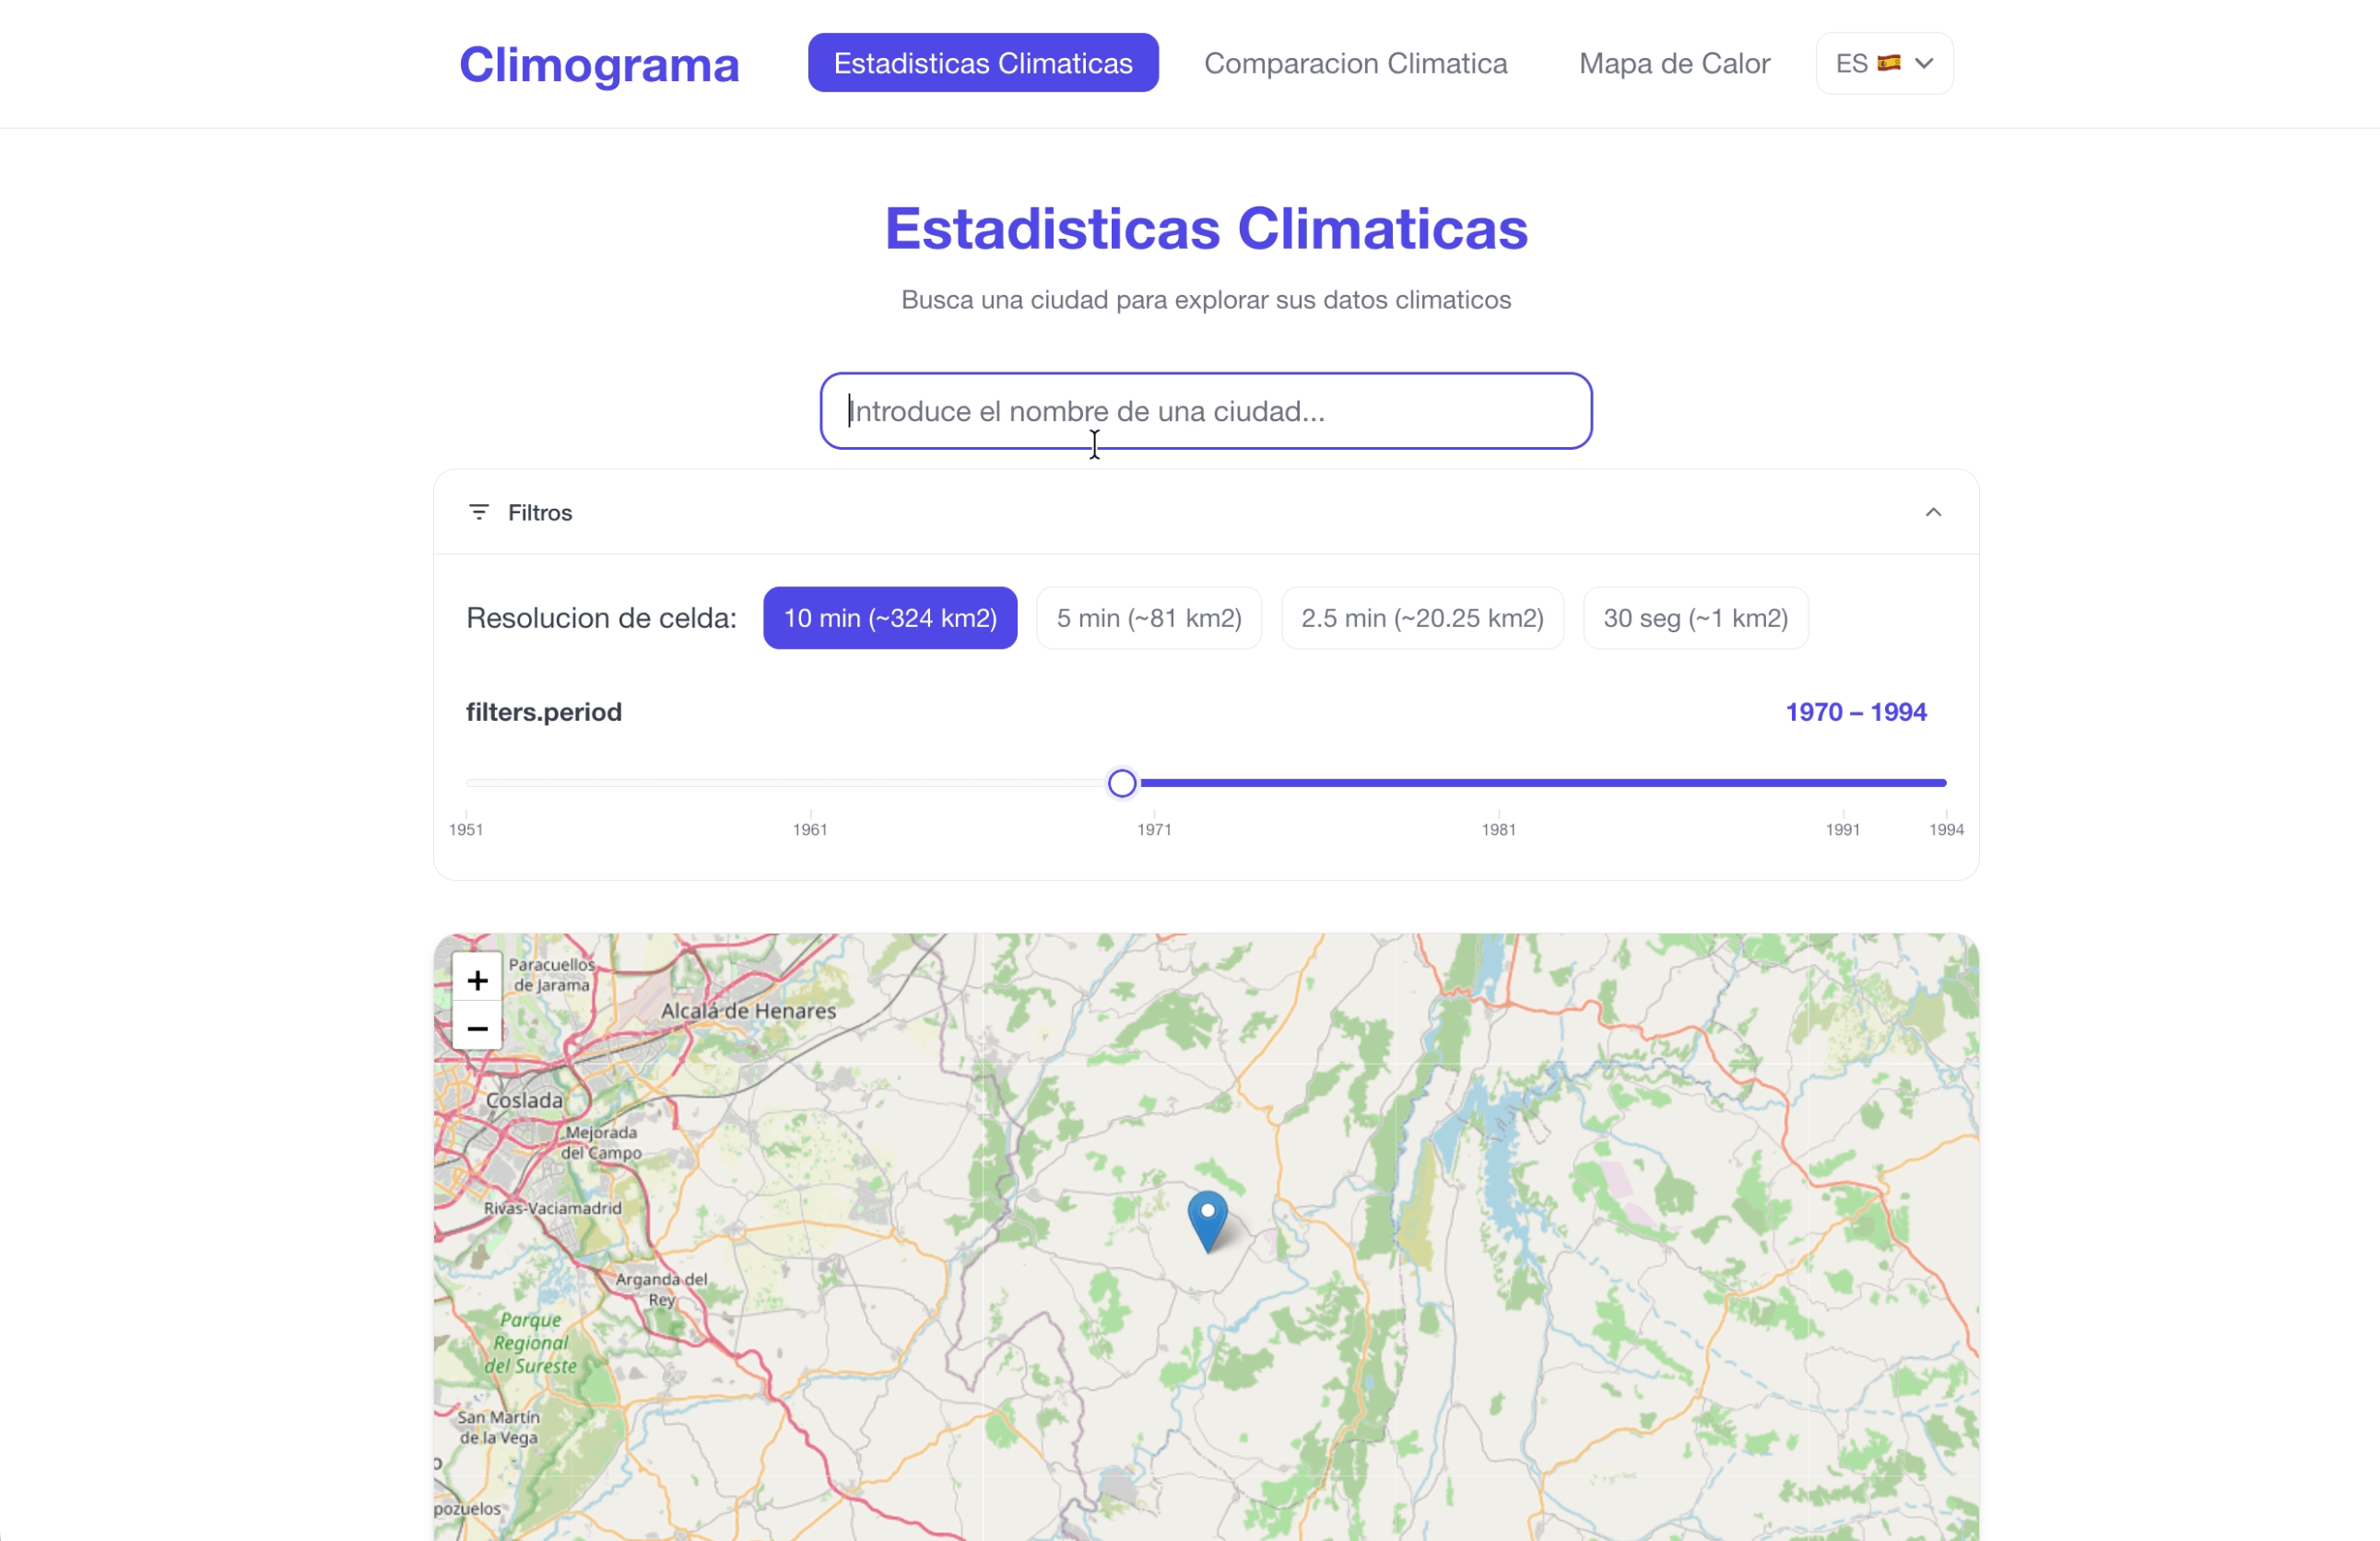
\includegraphics[width=0.9\textwidth]{Images/climatica-v1.png}
  \caption{Early prototype of Climatica (first iteration). The filter panel
    expanded below the search bar; the single page combined map, chart, and
    controls without a persistent sidebar. This layout was later reorganised
    into a fixed sidebar and four separate pages.}
  \label{fig:proto_v1}
\end{figure}

\subsection{Functional Requirements}\label{APP_REQ_FUNC}

The following functional requirements were established through the iterative
process described above. Requirements marked with an asterisk (*) emerged during
later review meetings rather than at the outset.

\begin{enumerate}
  \item \textbf{FR1 --- City search by name.} The user shall be able to type a
    city name and select from a ranked list of matching populated places.

  \item \textbf{FR2 --- Location by coordinates.} The user shall be able to
    enter a latitude/longitude pair directly in the search bar to retrieve
    climate data for any arbitrary point.

  \item \textbf{FR3 --- Location by map click.} The user shall be able to click
    any point on the interactive map to retrieve climate data for that location.

  \item \textbf{FR4 --- Use my location.} The user shall be able to use the
    browser's geolocation API to centre the map and retrieve climate data for
    their current position.

  \item \textbf{FR5 --- City climate profile.} For a selected city, the
    application shall display monthly minimum temperature, maximum temperature,
    average temperature, and precipitation, together with summary statistics
    (annual mean temperature, total precipitation, altitude, number of arid
    months).

  \item \textbf{FR6 --- Standard climograph.} The city climate profile shall be
    available as a standard bar-and-line chart showing precipitation bars and
    temperature lines.

  \item \textbf{FR7 --- Walter-Lieth climatogram.*} The city climate profile
    shall also be available as a Walter-Lieth diagram with correct arid/humid
    area shading.

  \item \textbf{FR8 --- City comparison.*} The user shall be able to select two
    cities and view their climate profiles side by side on shared axes, together
    with summary statistics and derived insights (warmer city, more rainfall,
    hottest month, coldest month).

  \item \textbf{FR9 --- Period comparison.*} The user shall be able to select
    one city and compare its climate across two to five time references ---
    either two 30-year climate normals or up to five individual weather years
    --- with trend indicators showing the direction and magnitude of change.

  \item \textbf{FR10 --- Regional heatmap.} The user shall be able to draw a
    bounding box or freeform polygon on the map and view a spatially resolved
    heatmap of any climate variable for any selected month.

  \item \textbf{FR11 --- Filter controls.} The user shall be able to filter all
    views by dataset (Climate / Weather), time period or year, climate variables,
    grid resolution, and month, with invalid combinations automatically disabled.

  \item \textbf{FR12 --- Data export.} The user shall be able to export chart
    data as CSV and as a PNG image.

  \item \textbf{FR13 --- Internationalisation.} The interface shall be available
    in English, Spanish, and Ukrainian, with city names displayed in the active
    language.
\end{enumerate}

\subsection{Non-Functional Requirements}\label{APP_REQ_NONFUNC}

\begin{enumerate}
  \item \textbf{NFR1 --- No registration.} The application shall be usable
    without creating an account.

  \item \textbf{NFR2 --- Secure API key handling.} The WorldClim Bearer token
    shall never be exposed to the browser; all SCRAPI calls shall be proxied
    through a server-side route handler.

  \item \textbf{NFR3 --- Shareable state.} Bounding box coordinates, city
    selections, and period selections shall be reflected in URL search parameters
    so that a specific view can be shared by copying the URL.

  \item \textbf{NFR4 --- Persistent preferences.} The user's last selected city,
    comparison cities, filter settings, and language preference shall survive a
    page reload.

  \item \textbf{NFR5 --- Type safety.} All API responses, domain data shapes,
    and component props shall be fully typed in TypeScript; no \texttt{any}
    types in production code.

  \item \textbf{NFR6 --- Code quality gate.} Every commit shall pass a CI check
    comprising TypeScript compilation, ESLint, and Prettier format verification,
    followed by a separate pipeline that runs the full unit and end-to-end test
    suites.
\end{enumerate}

% ─── 3.2 Architecture ─────────────────────────────────────────────────────────
\section{Architecture}\label{APP_ARCH}

\subsection{Evolution of the Architecture}\label{APP_ARCH_EVOLUTION}

Climatica was originally built as a pure React single-page application (SPA)
bundled with Vite and deployed as a static file set. In this version, all
external API calls --- to SCRAPI and Wikidata --- were issued directly from the
browser. City search relied entirely on the Wikidata \texttt{wbsearchentities}
and SPARQL endpoints to resolve user queries to geographic coordinates.

This approach proved adequate for a prototype but introduced two significant
limitations as the application matured. First, Wikidata applies soft-throttling
to high-frequency queries from a single origin: under interactive typing, the
search bar could exhaust the allowed request rate, causing intermittent failures
with no clean recovery path. Second, the Wikidata pipeline offered limited
control over result ranking; surfacing the most relevant city for a given query
required heuristics built on top of a remote API that could not be tuned or
extended without changing the query logic.

To address both issues, the architecture was redesigned around Next.js~16 with
the App Router. The key changes were: (1)~replacing the Wikidata city-search
pipeline with a locally hosted Apache Solr index, giving full control over
ranking, tokenisation, and query performance; (2)~introducing server-side route
handlers that proxy all SCRAPI and Solr requests, keeping the WorldClim Bearer
token off the client; and (3)~adding a Redis caching layer in front of both
Solr and SCRAPI to reduce latency for repeated queries.

Table~\ref{tab:arch_comparison} summarises the key differences between the two
versions.

\begin{table}[H]
  \centering
  \caption{Architecture comparison: React SPA (v1) vs.\ Next.js full-stack (v2).}
  \label{tab:arch_comparison}
  \small
  \begin{tabular}{p{3.2cm}p{4.8cm}p{4.8cm}}
    \toprule
    \textbf{Aspect} & \textbf{React SPA (v1)} & \textbf{Next.js (v2)} \\
    \midrule
    Framework       & React~18 + Vite        & Next.js~16 (App Router) \\
    City search     & Wikidata SPARQL pipeline & Apache Solr (GeoNames data) \\
    API calls       & Direct from browser    & Server-side route handlers \\
    API key exposure & Bearer token in browser & Server-only environment variable \\
    Caching         & TanStack Query (client) & Redis (server) + TanStack Query \\
    Infrastructure  & Static files only      & Docker Compose (Solr + Redis) \\
    Routing         & React Router           & Next.js file-system routing \\
    i18n            & i18next + react-i18next & next-intl \\
    Testing         & None                   & Vitest (unit) + Playwright (E2E) \\
    CI/CD           & None                   & GitHub Actions (2 pipelines) \\
    \bottomrule
  \end{tabular}
  \normalsize
\end{table}

\subsection{High-Level Architecture}\label{APP_ARCH_HIGH}

Figure~\ref{fig:arch_v1} shows the original React SPA architecture, retained
here for reference. The browser communicated directly with three external
services: SCRAPI, Wikidata, and OpenStreetMap. No server component existed;
the Bearer token was stored in a client-side environment variable.

\begin{figure}[H]
  \centering
  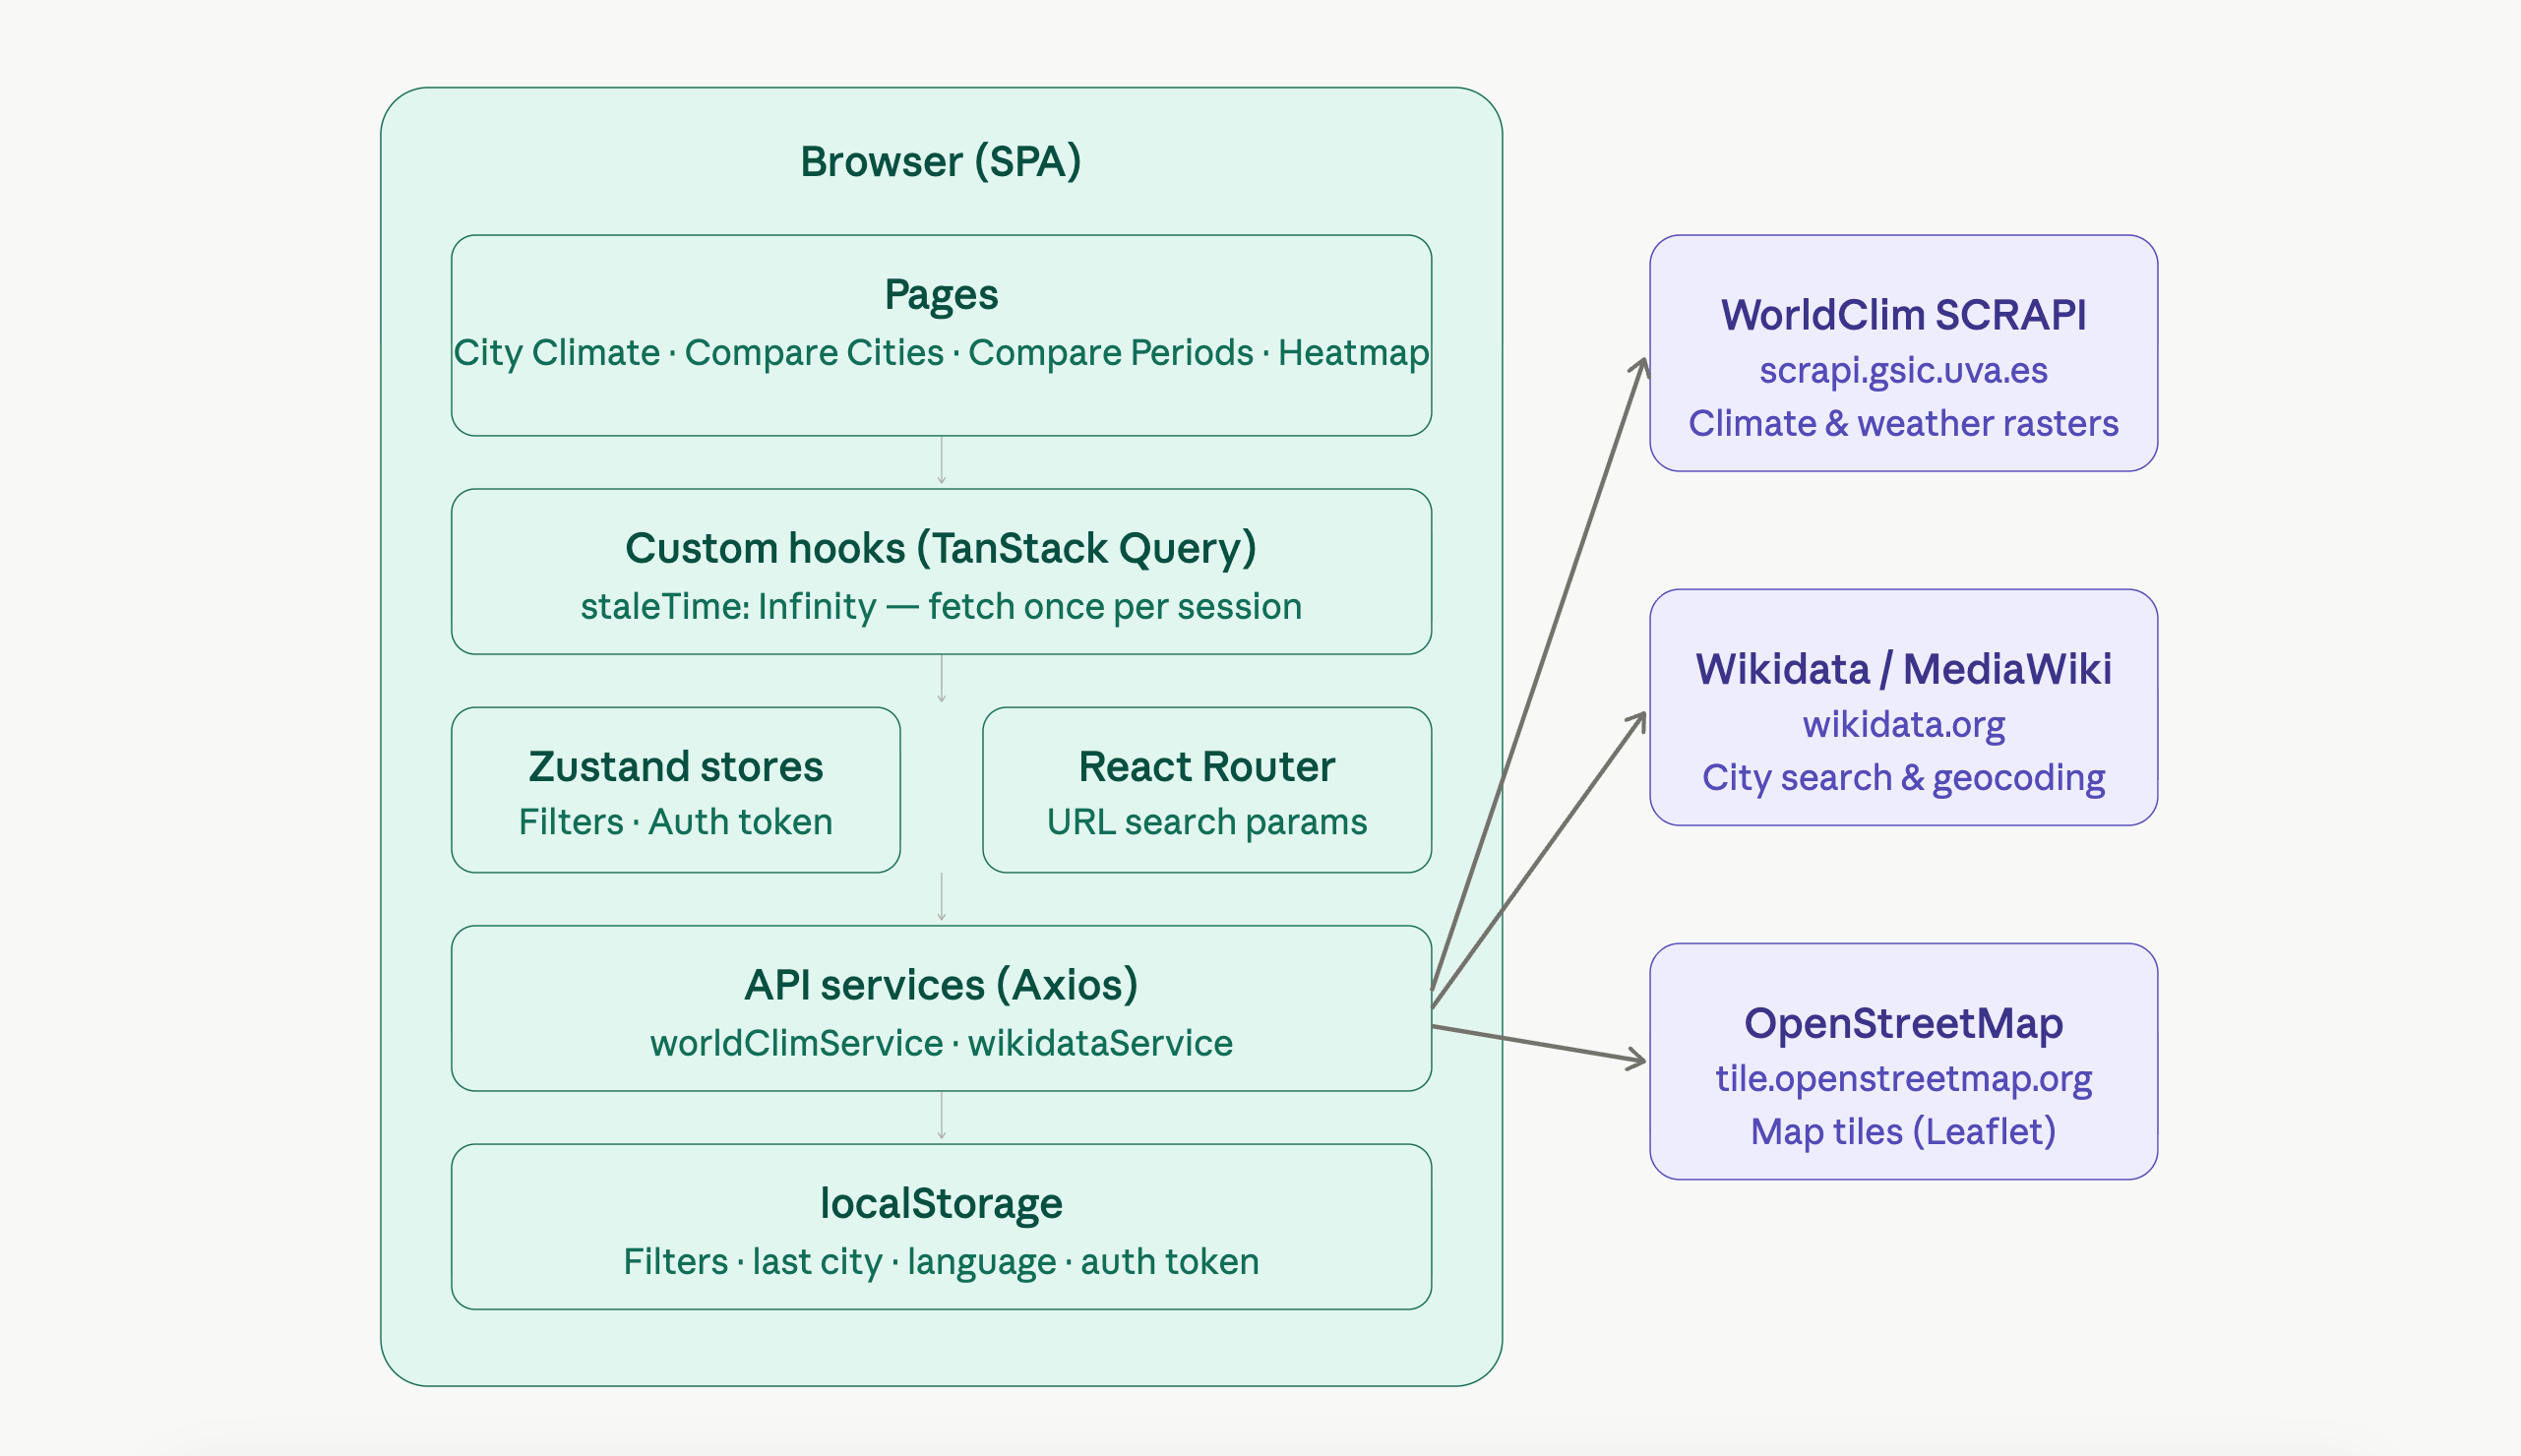
\includegraphics[width=0.85\textwidth]{Images/climatica-architecture-v1.png}
  \caption{Original React SPA architecture (v1). All API calls originate in
    the browser. The WorldClim Bearer token is exposed as a client-side
    environment variable. City search is handled by the Wikidata pipeline.}
  \label{fig:arch_v1}
\end{figure}

Figure~\ref{fig:arch_v2} shows the Next.js architecture. The browser
communicates exclusively with the Next.js server via \texttt{/api/*} route
handlers. The server contacts SCRAPI, Solr, and Wikidata (the last only for
reverse geocoding when the user enters coordinates manually or clicks the map).
Redis sits between the route handlers and the upstream services, absorbing
repeated queries. Map tiles are the only resource still fetched directly by the
browser, as they require no authentication.

\begin{figure}[H]
  \centering
  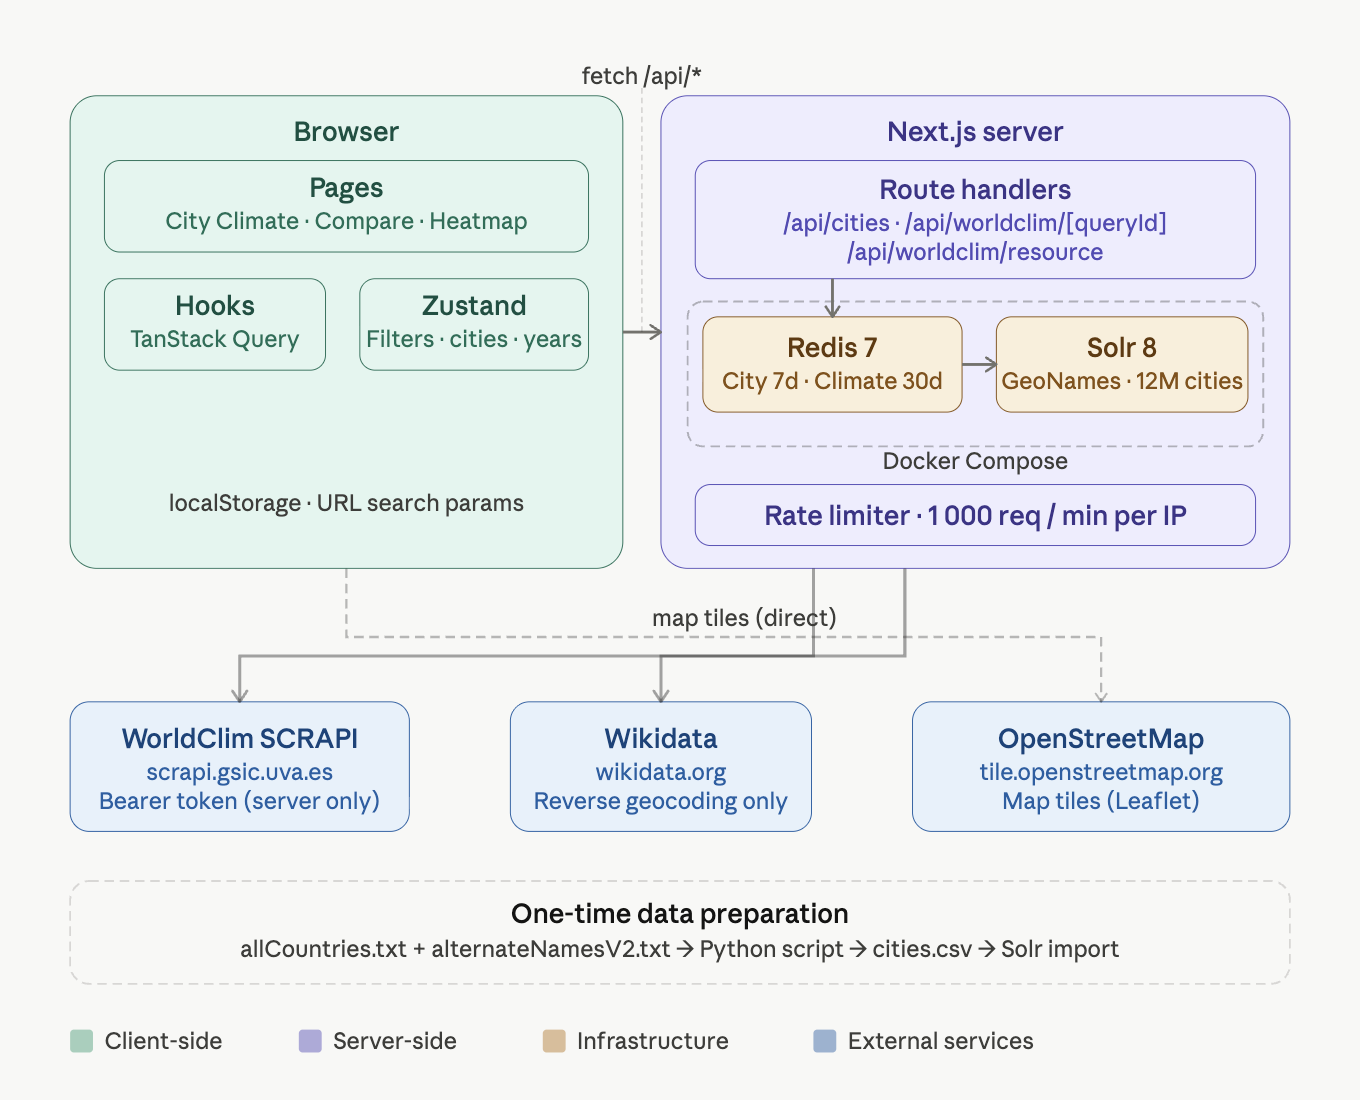
\includegraphics[width=0.85\textwidth]{Images/climatica-architecture-v2.png}
  \caption{Next.js full-stack architecture (v2). The browser communicates only
    with Next.js route handlers. Redis caches Solr and SCRAPI responses
    server-side. The WorldClim Bearer token never reaches the client. Wikidata
    is retained for reverse geocoding (coordinate input and map clicks).
    Map tiles are fetched directly from OpenStreetMap by Leaflet.}
  \label{fig:arch_v2}
\end{figure}

\subsection{City Search: from Wikidata to Solr}\label{APP_ARCH_SOLR}

In the original architecture, city search was implemented as a two-step
Wikidata pipeline: a \texttt{wbsearchentities} call followed by a SPARQL
filter query. While this approach required no local infrastructure, it was
subject to Wikidata's soft-throttling policy and offered no way to tune
ranking without modifying the SPARQL query.

The replacement pipeline uses GeoNames~\cite{geonames} as the data source.
GeoNames distributes two datasets: \texttt{allCountries.txt} (approximately
400\,MB, containing over 12~million place records with coordinates, feature
codes, and population figures) and \texttt{alternateNamesV2.txt} (approximately
200\,MB, containing localised place names in hundreds of languages). Both files
are placed in \texttt{docker/solr/data/} alongside an
\texttt{iso-languagecodes.txt} reference file.

A Python preprocessing script (\texttt{docker/solr/scripts/prepare\_data.py})
merges the two main files, filters records to populated places only (GeoNames
feature class \texttt{P}, covering the codes \texttt{PPL}, \texttt{PPLA},
\texttt{PPLA2}--\texttt{PPLA5}, and \texttt{PPLC}), and writes a single
\texttt{cities.csv} file with the following fields per record: GeoNames
identifier, English name, Ukrainian name, Spanish name, latitude, longitude,
feature code, country code, and population. For the name fields, the script
applies a priority rule: the preferred alternate name for a given language is
taken first; if none exists, the ASCII name is used, and the original default
name is the last resort.

The resulting CSV is imported into an Apache Solr~8 core named
\texttt{cities}. The Solr schema defines three text fields for multilingual
name matching (\texttt{label\_en}, \texttt{label\_uk}, \texttt{label\_es})
and enables trigram-based sub-word indexing via a custom
\texttt{solrconfig.xml}. Trigrams allow partial-word matches: the query
\texttt{``val''} returns \texttt{Valladolid} without requiring a dedicated
prefix index or a minimum query length constraint.

At query time, the \texttt{SolrService} selects the label field that
corresponds to the active locale (\texttt{getLabelField}), constructs a
parameterised Solr query, and maps each document to a \texttt{TWikidataCity}
object that is compatible with the existing client-side data shapes. The query
is routed through the \texttt{/api/cities} Next.js route handler, which
consults Redis before forwarding to Solr.

Wikidata is still used for two closely related tasks: reverse geocoding when
the user clicks the map, and coordinate lookup when the user types a
latitude/longitude pair directly. Both cases call
\texttt{WikidataService.findNearestCityByCoordinates}, which issues a
GeoSearch request with a 10\,km radius. Because these operations are
low-frequency and point-in-time, the soft-throttling constraint that affects
interactive text search does not apply.

\subsection{Caching Strategy with Redis}\label{APP_ARCH_REDIS}

A Redis~7 instance running in Docker provides server-side caching for all
upstream requests. The caching layer is implemented as a typed
\texttt{RedisClient} singleton (using \texttt{ioredis}) with three distinct
strategies defined in \texttt{REDIS\_STRATEGIES}:

\begin{itemize}
  \item \textbf{City search.} Results are cached by query string and language.
    Short queries (fewer than four characters) use a reduced TTL because
    they produce broad result sets that become stale faster as the user
    continues typing. For longer queries, a per-key hit counter is incremented
    on every cache miss via a Redis \texttt{INCR} command; once a query crosses
    the \texttt{popularThreshold}, it is promoted to a longer TTL to retain
    frequently requested results in memory.

  \item \textbf{Climate data.} SCRAPI responses are cached by the full
    request URL. The same popularity-based TTL promotion applies: the first
    requests for a given location--period--variable combination use a standard
    30-day TTL; repeated requests extend the TTL automatically.

  \item \textbf{Nearest city (reverse geocoding).} Results are cached by
    rounded coordinate pair with a fixed TTL, since the nearest city to a
    given point does not change.
\end{itemize}

The \texttt{RedisClient} uses lazy connection, offline queuing, and
exponential-backoff retry (up to three attempts, at 100\,ms, 200\,ms, and
400\,ms) so that a Redis restart does not crash the application --- uncached
requests are simply served directly from Solr or SCRAPI until the connection
is restored.

Client-side, TanStack Query continues to operate with
\texttt{staleTime:~Infinity} for all WorldClim data, providing a second
caching layer within the browser session and preventing redundant calls to
the \texttt{/api/worldclim} route handlers.

\subsection{Infrastructure and Deployment}\label{APP_ARCH_INFRA}

Both Solr and Redis are managed through a single Docker Compose file at
\texttt{docker/docker-compose.yml}. The file defines two services:

\begin{itemize}
  \item \textbf{climatica-solr} --- Apache Solr~8 with a custom
    \texttt{solrconfig.xml} mounted from the repository. The container
    auto-creates the \texttt{cities} core on first start via the
    \texttt{solr-precreate} command entry point. A health check polls
    \texttt{/solr/cities/admin/ping} every 30 seconds with up to five
    retries.
  \item \textbf{climatica-redis} --- Redis~7 Alpine with append-only
    persistence (\texttt{redis-server --appendonly yes}) so that the
    cache survives container restarts. A health check runs
    \texttt{redis-cli ping} every 10 seconds.
\end{itemize}

Named volumes (\texttt{solr\_data}, \texttt{redis\_data}) persist index and
cache data across container lifecycles. The full developer workflow is
encapsulated in four \texttt{npm} scripts: \texttt{docker:up},
\texttt{docker:down}, \texttt{docker:reboot}, and \texttt{docker:logs}.
City data is imported into Solr via a two-step \texttt{npm run solr:reindex}
command that first POSTs the schema definition and then copies and imports the
\texttt{cities.csv} file into the running container. Indexing approximately
12~million records takes around three minutes on first run.

The application is deployed on the Universidad de Valladolid server. The
Next.js production server runs behind an Nginx reverse proxy that handles
SSL termination and forwards requests to port~3000.

\subsection{Folder Structure}\label{APP_ARCH_FOLDERS}

The Next.js source tree follows the App Router convention. The top-level
directories under \texttt{src/} are:

\begin{itemize}
  \item \texttt{app/} --- file-system routes. Each page directory contains
    a server component entry point and a client component view. The
    \texttt{app/api/} subdirectory contains the three route handlers:
    \texttt{cities/route.ts} (city search via Redis\,$\to$\,Solr),
    \texttt{worldclim/[queryId]/route.ts} (SCRAPI query proxy with rate
    limiting), and \texttt{worldclim/resource/route.ts} (SCRAPI resource
    proxy with Redis caching).

  \item \texttt{components/} --- shared UI components reused across pages,
    including the sidebar filter panel, chart components, skeleton loading
    placeholders, and the Leaflet map container (dynamically imported with
    \texttt{ssr:~false} to avoid the server-side rendering incompatibility
    of the Leaflet library).

  \item \texttt{hooks/} --- custom React hooks: \texttt{data/} for TanStack
    Query data-fetching hooks, \texttt{persisted/} for Zustand-backed
    state, and \texttt{ui/} for theme, geolocation, and drawing mode state.

  \item \texttt{libs/} --- server-only modules annotated with
    \texttt{import "server-only"}: \texttt{redis/} (client singleton and
    caching strategies), \texttt{api/} (Axios instance), and
    \texttt{services/} (\texttt{SolrService}, \texttt{WikidataService},
    \texttt{WorldClimService}).

  \item \texttt{types/}, \texttt{constants/}, \texttt{utils/} --- pure
    TypeScript with no framework imports. All magic values are declared as
    named constants; naming follows a strict convention: \texttt{T} prefix
    for types, \texttt{E} prefix for enums, \texttt{*.constant.ts} for
    constants.
\end{itemize}

\subsection{Data Flow}\label{APP_ARCH_FLOW}

The data flow follows a strict unidirectional pattern:

\begin{center}
\texttt{Component \textrightarrow\ Hook \textrightarrow\ fetch /api/* \textrightarrow\
Route Handler \textrightarrow\ Redis \textrightarrow\ Solr / SCRAPI}
\end{center}

Client components never call external services directly --- all requests go
through \texttt{/api/} route handlers. This boundary ensures that
authentication credentials remain server-side and that the Redis cache is
always consulted before any upstream request is made.

\subsection{State Management}\label{APP_ARCH_STATE}

State is stratified by lifetime and sharing scope, as shown in
Table~\ref{tab:state}. This stratification avoids the common anti-pattern of
storing everything in a single global store, which makes it difficult to reason
about what triggers re-renders and why.

\begin{table}[H]
  \centering
  \caption{State management strategy in Climatica.}
  \label{tab:state}
  \small
  \begin{tabular}{p{4cm}p{3.5cm}p{5.5cm}}
    \toprule
    \textbf{State type} & \textbf{Location} & \textbf{Rationale} \\
    \midrule
    Server data (WorldClim, Solr) & TanStack Query &
      Automatic deduplication; \texttt{staleTime: Infinity} since climate
      data never changes \\
    Global filter settings & Zustand + \texttt{persist} &
      Survives page navigation; persisted to \texttt{localStorage} \\
    Selected weather years & Zustand + \texttt{persist} &
      Up to five years retained across sessions \\
    City sync setting & Zustand + \texttt{persist} &
      Opt-out toggle; default on \\
    Shareable UI state & URL search params &
      Allows bookmarking and sharing specific views \\
    Last selected city & \texttt{usePersistedCity} hook &
      Survives hard reload without polluting URL \\
    Comparison cities & \texttt{usePersistedComparisonCities} hook &
      Separate store for City~A / City~B \\
    UI-only state & Local \texttt{useState} &
      Scoped to component; no need to share \\
    Derived data & Computed at render time &
      Never stored; computed from props or query results \\
    \bottomrule
  \end{tabular}
  \normalsize
\end{table}

\textbf{Cross-page city synchronisation.} A configurable sync feature
propagates the selected city across pages when enabled. The setting is stored
in the Zustand \texttt{filtersStore} under the key \texttt{syncCity}
(default: on) and is toggled via a \texttt{ToggleSwitch} in a collapsible
Settings section of the sidebar. When the user selects a city on any page,
the sync logic updates both \texttt{usePersistedCity} (used by City Climate
and Compare Periods) and \texttt{usePersistedComparisonCities.cityA} (used
by Compare Cities), so that the selected city immediately appears as the
primary city on all other pages. City~B on Compare Cities is never synced ---
only City~A participates in the cross-page propagation. The sync is guarded
by a \texttt{hasHydrated} flag that prevents race conditions during the
initial Zustand store rehydration from \texttt{localStorage}.

\subsection{Draft Filter Pattern}\label{APP_ARCH_DRAFT}

The global sidebar maintains a \emph{draft} copy of the filter state separate
from the committed Zustand store. Users adjust chips and dropdowns freely; the
draft is validated with Zod and committed to the store only when the user clicks
``Apply filters''. This prevents partial or invalid filter states from triggering
expensive API calls mid-edit.

The draft also enforces domain constraints eagerly: switching the dataset to
\emph{Weather} automatically strips the three variables unavailable in that
dataset (\texttt{srad}, \texttt{wind}, \texttt{vapr}) and downgrades the
30-second grid to 2.5-minute resolution, because weather rasters are not
available at 30-second resolution.

\subsection{Skeleton Loading States}\label{APP_ARCH_SKELETONS}

Every section of the interface that depends on asynchronous data has a
dedicated skeleton loading placeholder. Five skeleton components --- all using
Tailwind's \texttt{animate-pulse} class --- cover the main content areas:
\texttt{ChartSkeleton} (a twelve-bar animated placeholder that matches the
approximate shape of a real climate chart), \texttt{MapSkeleton} (a tile-grid
layout with a centre pin indicator, available in \texttt{full} and
\texttt{mini} variants), \texttt{StatCardsSkeleton} (a responsive grid of
blank stat cards), \texttt{TableSkeleton} (a configurable table with a header
row and body rows), and \texttt{ComparisonTableSkeleton} (a fixed five-row
variant for the comparison stats grid).

Figure~\ref{fig:skeleton_loading} shows the Compare Cities page in its loading
state, where the minimap, statistics table, and chart are all replaced with
animated placeholders until data arrives from the route handlers.

\begin{figure}[H]
  \centering
  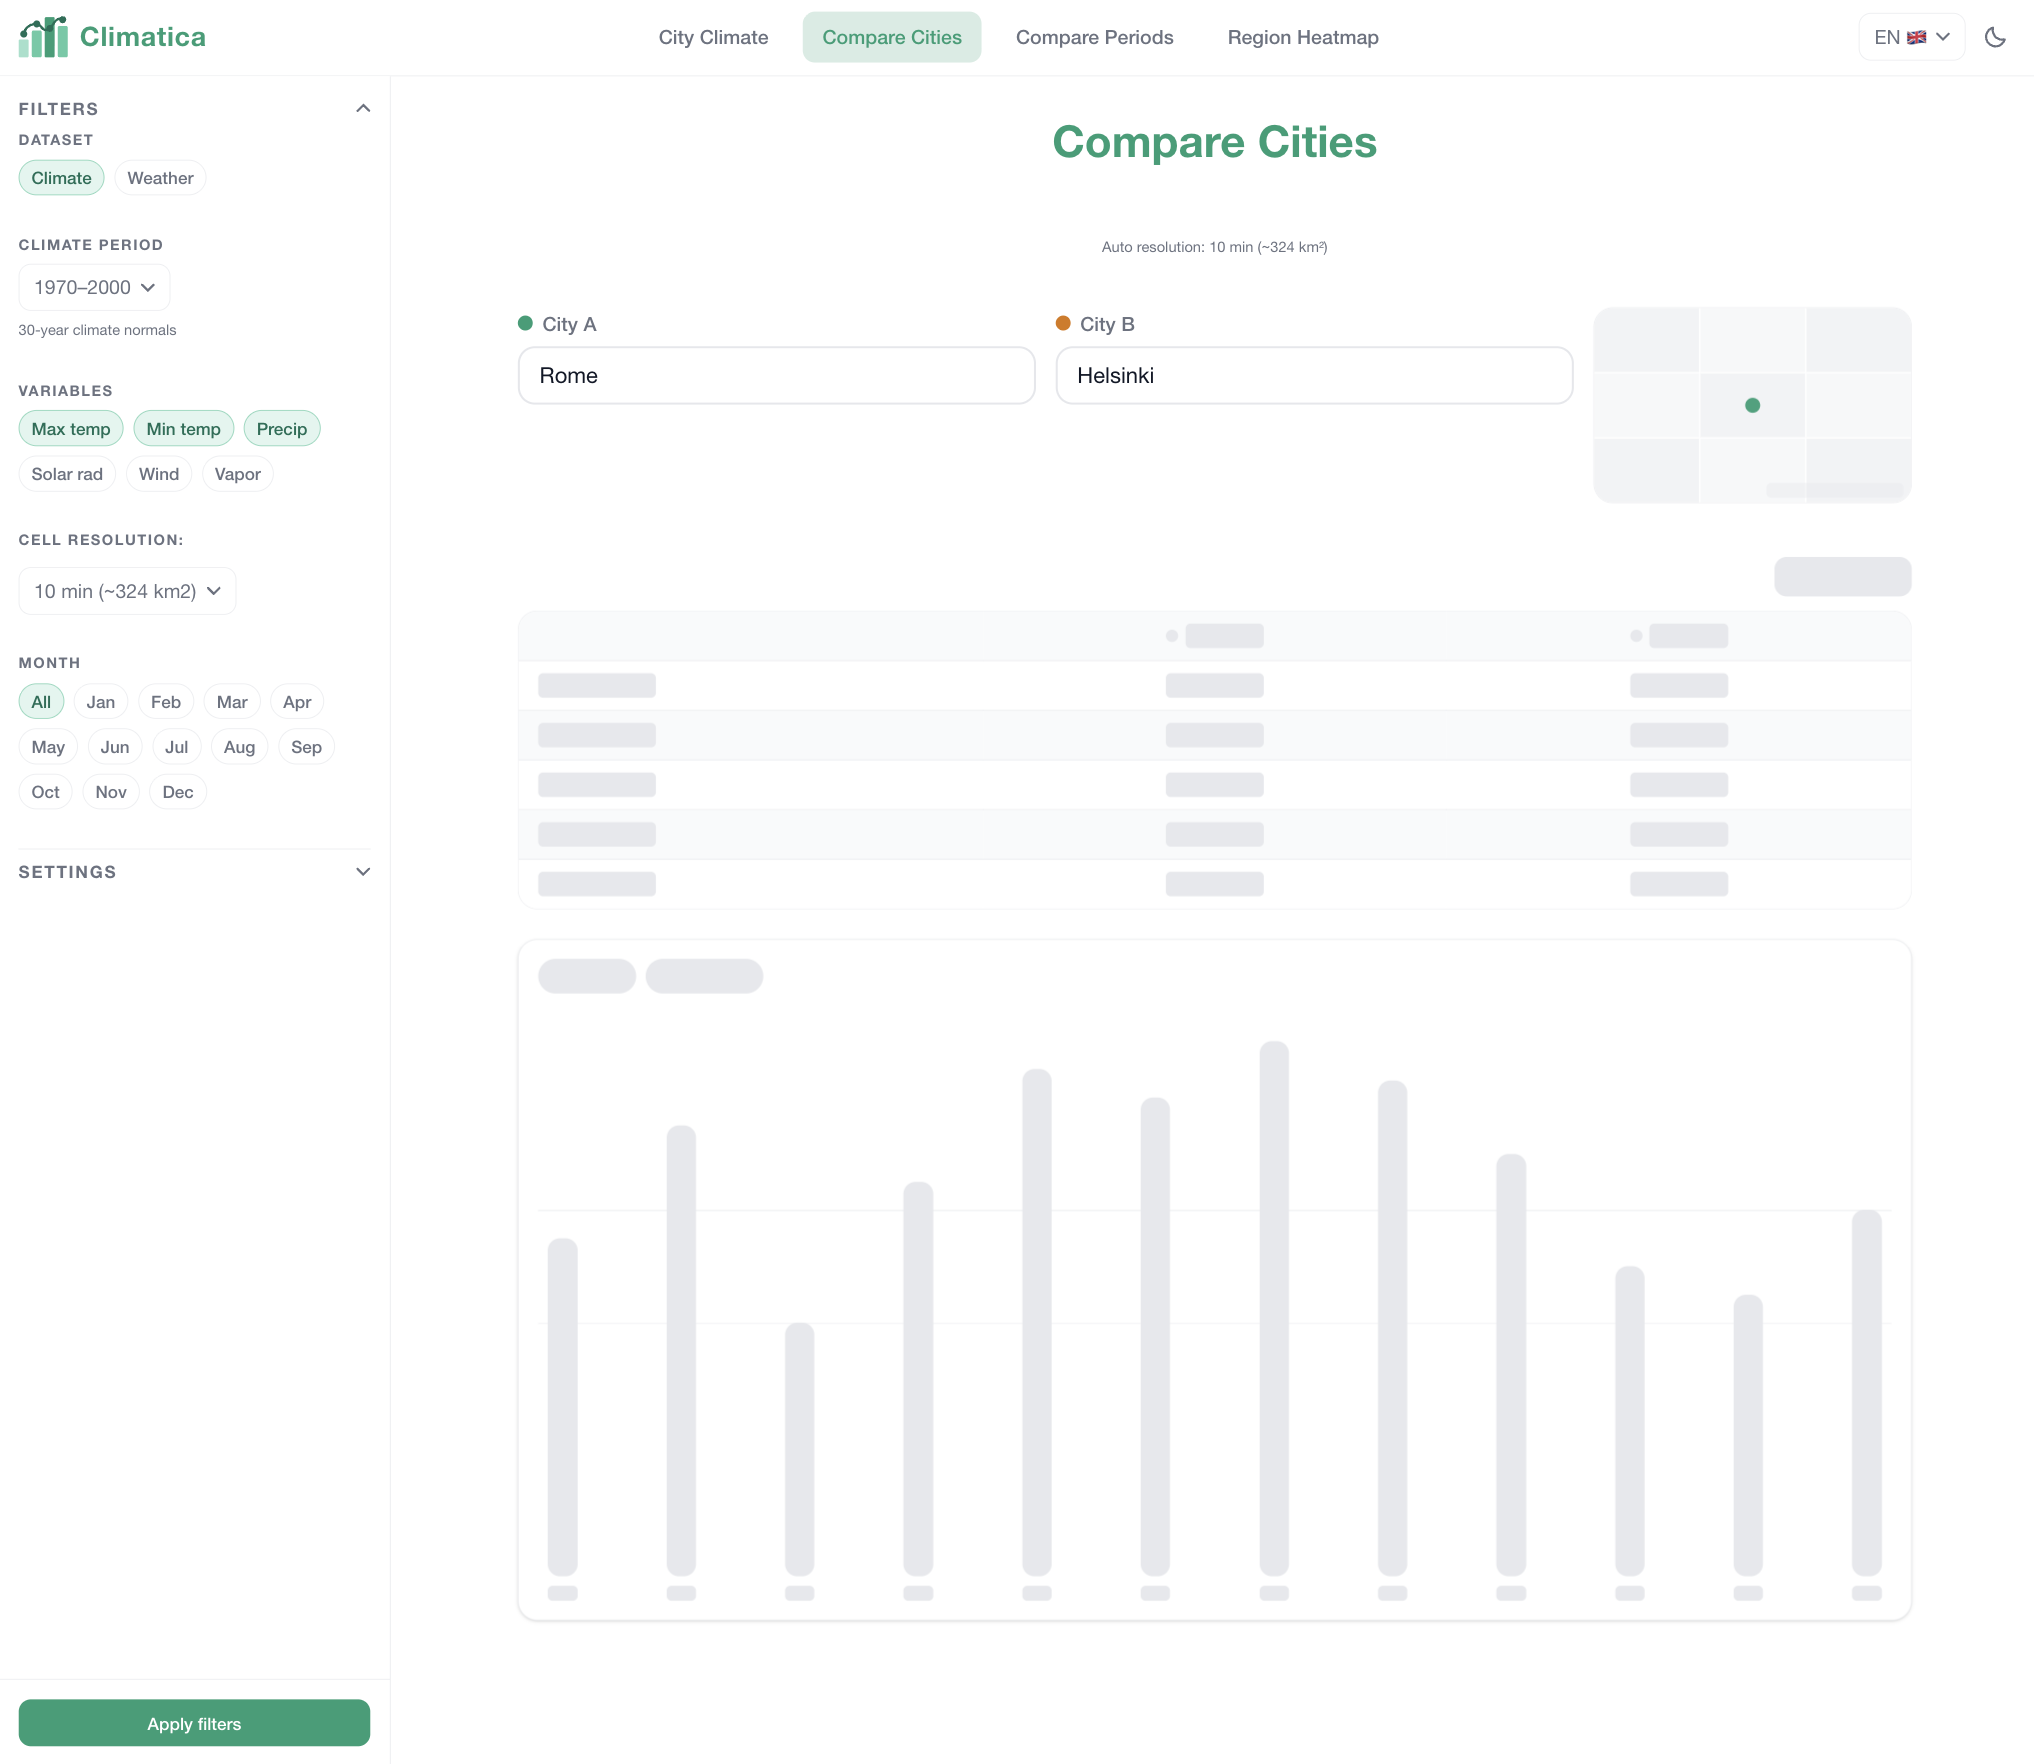
\includegraphics[width=0.9\textwidth]{Images/climatica-skeleton-loading-state.png}
  \caption{Compare Cities page in its loading state. The minimap, statistics
    table, and chart are replaced with animated skeleton placeholders. The map
    skeleton uses a tile-grid pattern with a central pin to mimic the appearance
    of a Leaflet map.}
  \label{fig:skeleton_loading}
\end{figure}

All Leaflet map components (\texttt{LeafletMap}, \texttt{MapCanvas},
\texttt{MiniMap}) are dynamically imported with \texttt{ssr:~false} and use
\texttt{MapSkeleton} as their loading fallback, which prevents a server-side
rendering crash caused by Leaflet's dependency on the browser \texttt{window}
object. In weather mode on the Compare Periods page, each year column in the
\texttt{MultiPeriodStatsTable} displays an individual skeleton placeholder
while its TanStack Query is still in-flight, so partial results become visible
progressively rather than blocking the entire table.
\subsection{Data Transformation and Domain Logic}\label{APP_ARCH_LOGIC}

A critical aspect of Climatica is the transformation of raw SCRAPI results into
meteorologically sound data structures. Unlike typical CRUD applications,
Climatica performs significant client-side computation to ensure scientific
accuracy.

\textbf{Aridity Calculation.} Following the Gaussen-Walter-Lieth climate
classification, a month is defined as arid when $P < 2T$, where $P$ is
precipitation in mm and $T$ is average temperature in $^\circ$C. This condition
is evaluated per month in \texttt{computeAridityPeriods} and is used both to
colour the bars in the standard climograph and to drive the filled areas in the
Walter-Lieth diagram.

\textbf{Dynamic Axis Scaling.} To maintain the $1{:}2$ ratio visually, the
application implements a custom scaling engine in \texttt{getWalterLiethScales}
(Listing~\ref{lst:scaling}). The algorithm ensures that both axes share the
same zero-baseline, that the precipitation maximum is exactly twice the
temperature maximum, and that tick values are rounded to the nearest multiple
of 5 for readability.

\begin{lstlisting}[language=TypeScript,
  caption={Walter-Lieth axis synchronisation.},
  label={lst:scaling}]
export function getWalterLiethScales(
  data: TMonthlyTemperature[]
): TWalterLiethScales {
  const tMax = Math.max(...data.map(d => (d.tmin + d.tmax) / 2));
  const tempMax = Math.ceil(tMax / 5) * 5;
  return {
    tempMin: 0, tempMax,
    precMin: 0, precMax: tempMax * 2,
  };
}
\end{lstlisting}

\subsection{Advanced SVG Visualisation}\label{APP_ARCH_SVG}

Implementing the Walter-Lieth climatogram required a custom SVG rendering
strategy, because standard charting libraries including Recharts do not
natively support ``area-between-curves'' fills with conditional colouring.

The solution uses SVG \texttt{clipPath} with the \textbf{even-odd winding rule}.
Two closed SVG paths are constructed --- $\mathit{Area}_T$ (the region from the
temperature curve down to the baseline) and $\mathit{Area}_P$ (the corresponding
precipitation region). A composite \texttt{clipPath} is built by concatenating
both paths. Because the even-odd rule fills a point only if it is enclosed by an
\emph{odd} number of component paths, the intersection region (where both curves
overlap) is automatically excluded from each fill. The result is pixel-perfect
arid and humid shading with no artefacts and no need to compute spline
intersection points explicitly.

Coordinate projection relies on Recharts~v3 internal hooks
(\texttt{useXAxisScale}, \texttt{useYAxisScale}), which expose the D3 scale
functions used internally by the chart. The custom \texttt{WLCustomized}
component uses these scales to convert data-space values into SVG pixel
coordinates, making the overlay fully responsive to window resizing.

% ─── 3.3 Quality Assurance ────────────────────────────────────────────────────
\section{Quality Assurance}\label{APP_QA}

\subsection{Testing Strategy}\label{APP_QA_TESTS}

The test suite is divided into two layers with clearly separated
responsibilities.

\textbf{Unit tests} are written with Vitest and cover the server-side modules
that contain the most business-critical logic: the Redis client and all three
caching strategies, the \texttt{/api/cities} and \texttt{/api/worldclim} route
handlers, \texttt{SolrService}, \texttt{WorldClimService}, URL utility functions,
and the city description generator. These tests run against mocked dependencies
and do not require Docker to be running, which keeps the feedback cycle fast
during development. Running \texttt{npm run test:coverage} produces a V8
coverage report that makes untested code paths immediately visible.

\textbf{End-to-end tests} are written with Playwright and cover five
user-visible flows: city search and result selection, climate data loading and
chart rendering, language switching across the three supported locales,
cross-page navigation, and the 404 not-found page. E2E tests require both
Docker services to be running and the Next.js development server to be active.

\subsection{CI/CD Pipelines}\label{APP_QA_CICD}

Two GitHub Actions workflows run on every push and pull request to the main
branch.

The \textbf{validation and build} pipeline executes the quality gate in
sequence: TypeScript compilation (\texttt{tsc --noEmit}), ESLint, Prettier
format check, unit tests with coverage, and a production build
(\texttt{next build}). This pipeline must pass before any merge is permitted.

The \textbf{E2E tests} pipeline spins up the Docker Compose stack (Solr and
Redis), waits for both health checks to pass, starts the Next.js server, and
then runs the full Playwright suite. Running E2E tests in CI catches regressions
in the full request path --- including route handler logic, Redis cache
behaviour, and Solr query construction --- that unit tests cannot detect in
isolation.

Together the two pipelines provide the safety net required for confident,
incremental deployment to the Universidad de Valladolid server.

% ─── 3.4 Technology Choices ───────────────────────────────────────────────────
\section{Technology Choices}\label{APP_TECH}

Table~\ref{tab:tech} lists the main technologies used in Climatica with their
versions and roles. The following paragraphs discuss the most significant
choices.

\begin{table}[H]
  \centering
  \caption{Technology stack of Climatica (v2).}
  \label{tab:tech}
  \small
  \begin{tabular}{llp{6.5cm}}
    \toprule
    \textbf{Technology} & \textbf{Version} & \textbf{Role} \\
    \midrule
    Next.js        & 16.2  & Full-stack framework; App Router; server-side
                             route handlers \\
    React          & 19.2  & Component model and declarative UI \\
    TypeScript     & 5.x   & Static typing with strict mode \\
    Tailwind CSS   & 4.2   & Utility-first styling \\
    TanStack Query & 4.43  & Client-side server-state management and
                             deduplication \\
    Zustand        & 5.0   & Lightweight global client state with
                             \texttt{persist} middleware \\
    Zod            & 4.3   & Runtime validation of filter inputs \\
    next-intl      & 4.12  & Internationalisation across three locales \\
    Leaflet + react-leaflet & 1.9 / 5.0 & Interactive map rendering \\
    Recharts       & 3.8   & SVG chart rendering; coordinate hooks for
                             Walter-Lieth overlay \\
    Axios          & 1.13  & HTTP client for client-side API calls \\
    Apache Solr    & 8     & City search index with trigram tokenisation \\
    Redis          & 7     & Server-side response cache \\
    ioredis        & 5.10  & Type-safe Redis client with retry logic \\
    html2canvas    & 1.4   & DOM-to-canvas rasterisation for PNG export \\
    Vitest         & 4.x   & Unit test runner \\
    Playwright     & 1.60  & End-to-end browser testing \\
    Docker Compose & ---   & Local orchestration of Solr and Redis \\
    \bottomrule
  \end{tabular}
  \normalsize
\end{table}

\textbf{Next.js.} The migration from Vite to Next.js was motivated by two
architectural requirements that a static SPA cannot satisfy: server-side route
handlers (needed to keep the WorldClim Bearer token off the client and to
front-run requests with Redis) and a richer deployment target that runs on the
university server alongside Nginx. The App Router model maps naturally to the
four-page structure of Climatica, and the clear server/client component boundary
makes it explicit which code runs where.

\textbf{Apache Solr.} Solr was chosen over alternatives (PostgreSQL full-text
search, Elasticsearch, Meilisearch) because it is mature, has first-class
support for trigram tokenisation via \texttt{solrconfig.xml} customisation, and
runs comfortably within the memory budget of the university server. The trigram
analyser enables partial-word matching --- a user typing \texttt{``mad''} sees
\texttt{Madrid} immediately --- without requiring a dedicated prefix index.

\textbf{Redis.} Redis was preferred over in-process caches because it persists
across server restarts and is shared across all Next.js worker processes. The
popularity-based TTL promotion strategy, which extends cache lifetime for
frequently requested queries, relies on an \texttt{INCR} counter that would not
be possible with a process-local cache.

\textbf{next-intl.} The original i18next integration was replaced by next-intl,
which integrates natively with the Next.js App Router middleware layer. Language
detection and locale routing are handled at the edge, so the correct locale is
available server-side on every request without a client-side hydration step.

\textbf{Vitest and Playwright.} Vitest was chosen over Jest for unit tests
because it shares the same ESM configuration as the rest of the project,
eliminating the need for a separate Babel transform. Playwright was chosen for
E2E tests because it supports all major browsers from a single configuration,
runs headlessly in CI with minimal setup, and provides a visual trace viewer
(\texttt{test:e2e:ui}) that makes debugging failed tests significantly faster.

% ─── 3.5 Prototype Description ────────────────────────────────────────────────
\section{Prototype Description}\label{APP_PROTO}

Climatica is organised into four pages accessible from the top navigation bar.
All pages share a persistent left sidebar containing the global filter controls.
The application supports light and dark themes; all screenshots in this section
show the light theme.

\subsection{City Climate}\label{APP_PROTO_CITY}

The City Climate page (Figure~\ref{fig:page_city_map}) is the primary entry
point of the application. The user searches for a city by name (backed by the
Solr index), enters coordinates directly, clicks a point on the map, or uses
the browser geolocation button. Upon selection, the page displays an interactive
Leaflet map centred on the selected city, with a pin marking the exact location
and a dashed rectangle outlining the WorldClim raster cell being queried,
together with four summary stat cards (average maximum temperature, average
minimum temperature, total annual precipitation, and elevation). Below the map,
the user can switch between two chart modes:

\begin{itemize}
  \item \textbf{Standard climograph} (Figure~\ref{fig:page_city_std}) ---
    precipitation as vertical bars (blue for humid months, yellow for arid
    months) and temperature as smooth lines.
  \item \textbf{Walter-Lieth diagram} (Figure~\ref{fig:page_city_wl}) ---
    precipitation and temperature as two smooth curves with filled areas
    indicating arid (yellow) and humid (blue) periods.
\end{itemize}

\begin{figure}[H]
  \centering
  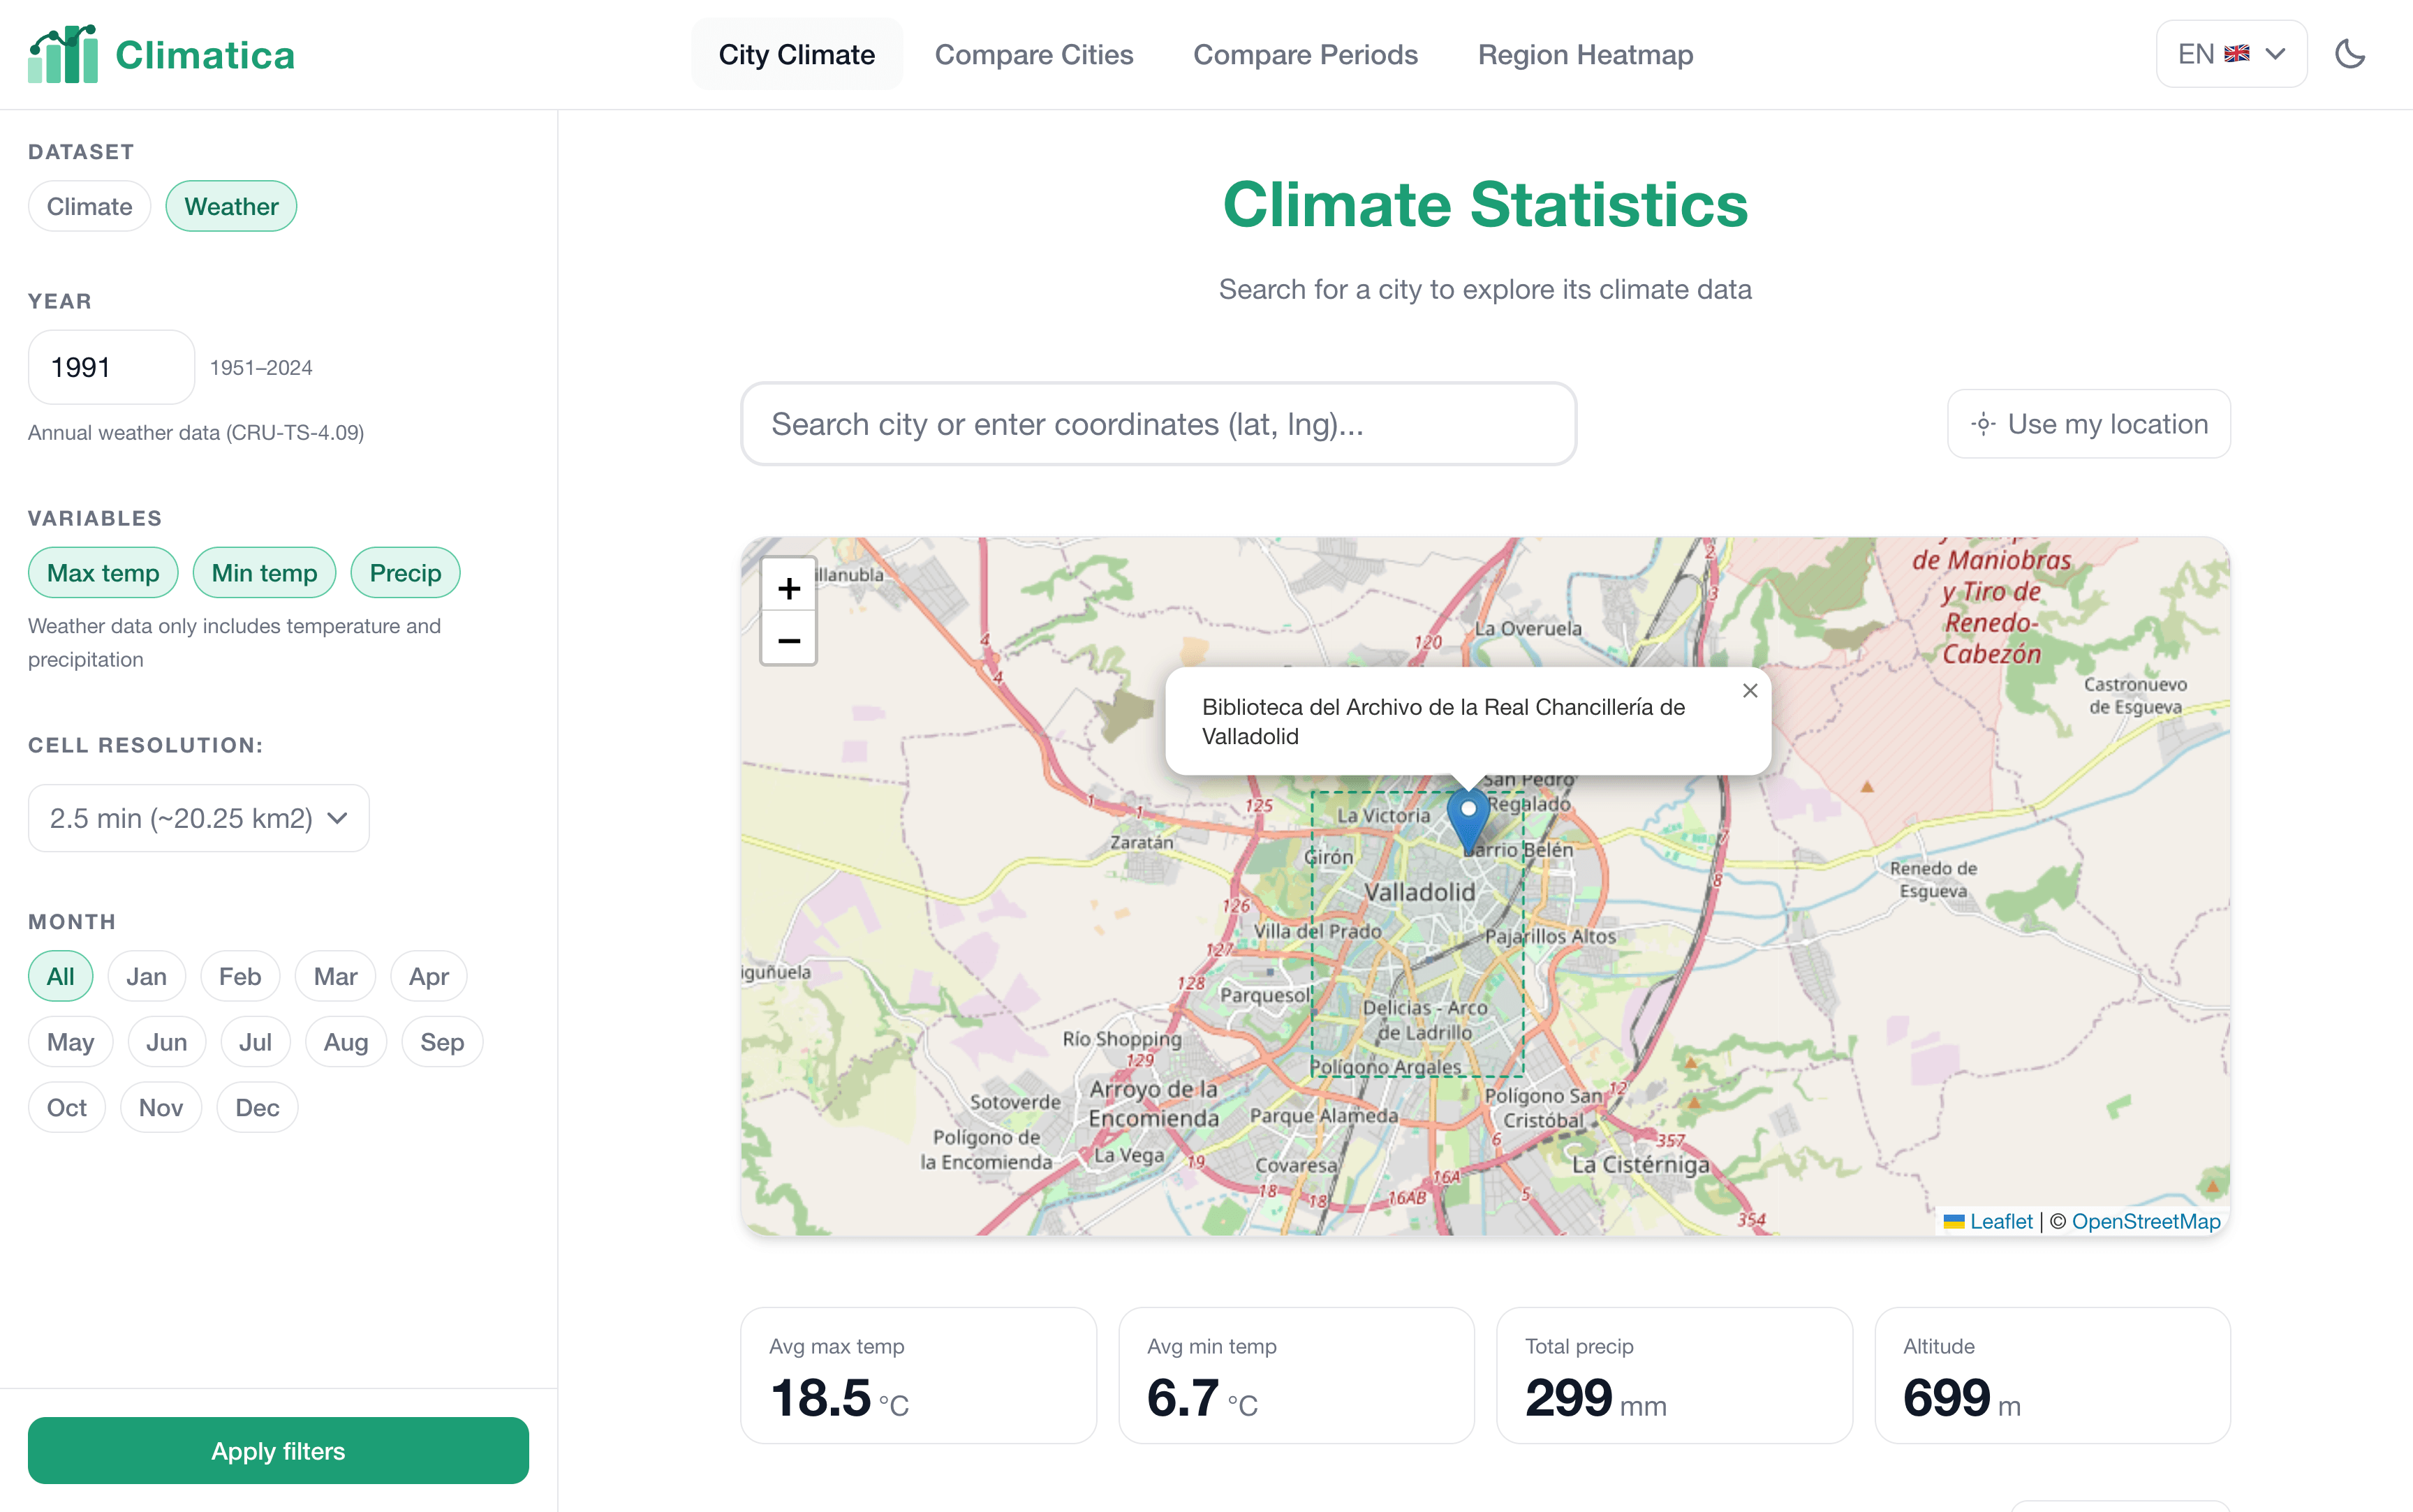
\includegraphics[width=0.9\textwidth]{Images/climatica-map.png}
  \caption{City Climate page --- map view with location pin, raster cell
    outline, and summary stat cards for Valladolid.}
  \label{fig:page_city_map}
\end{figure}

\begin{figure}[H]
  \centering
  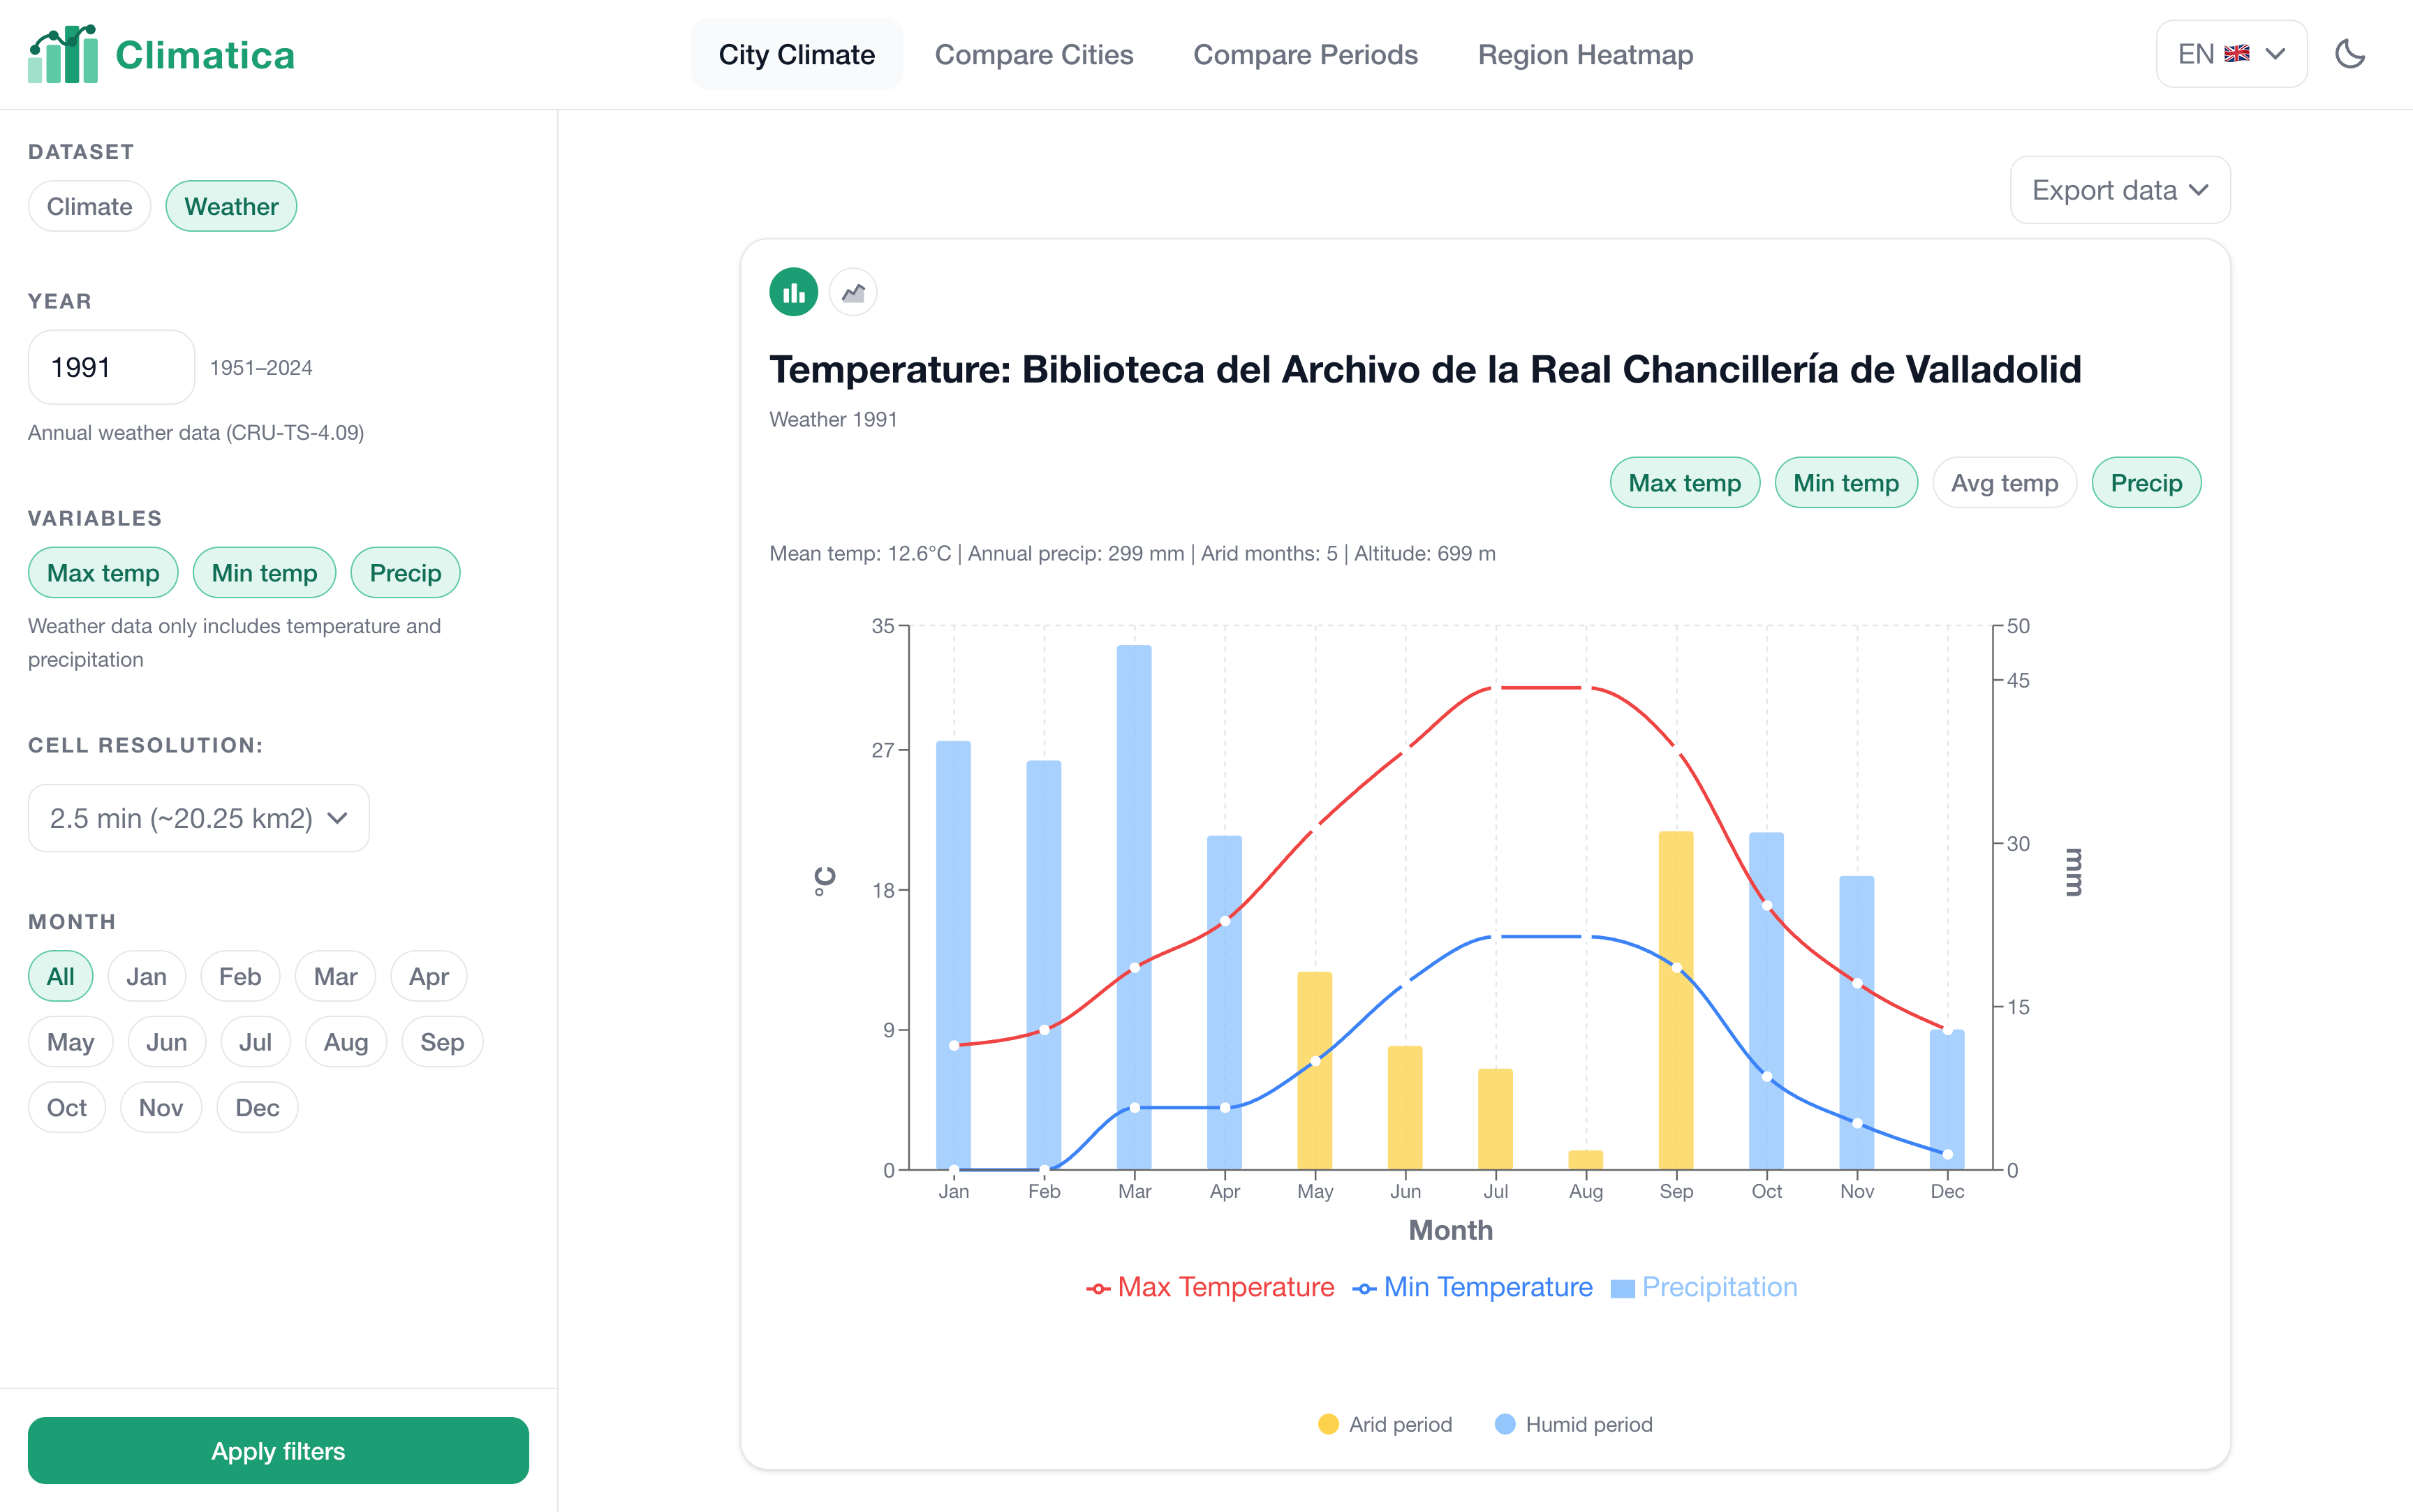
\includegraphics[width=0.9\textwidth]{Images/climatica-columns-graph.png}
  \caption{City Climate page --- standard climograph for Valladolid (weather
    dataset, year 1991). Precipitation is shown as bars; temperature as smooth
    lines. Blue bars indicate humid months; yellow bars indicate arid months.}
  \label{fig:page_city_std}
\end{figure}

\begin{figure}[H]
  \centering
  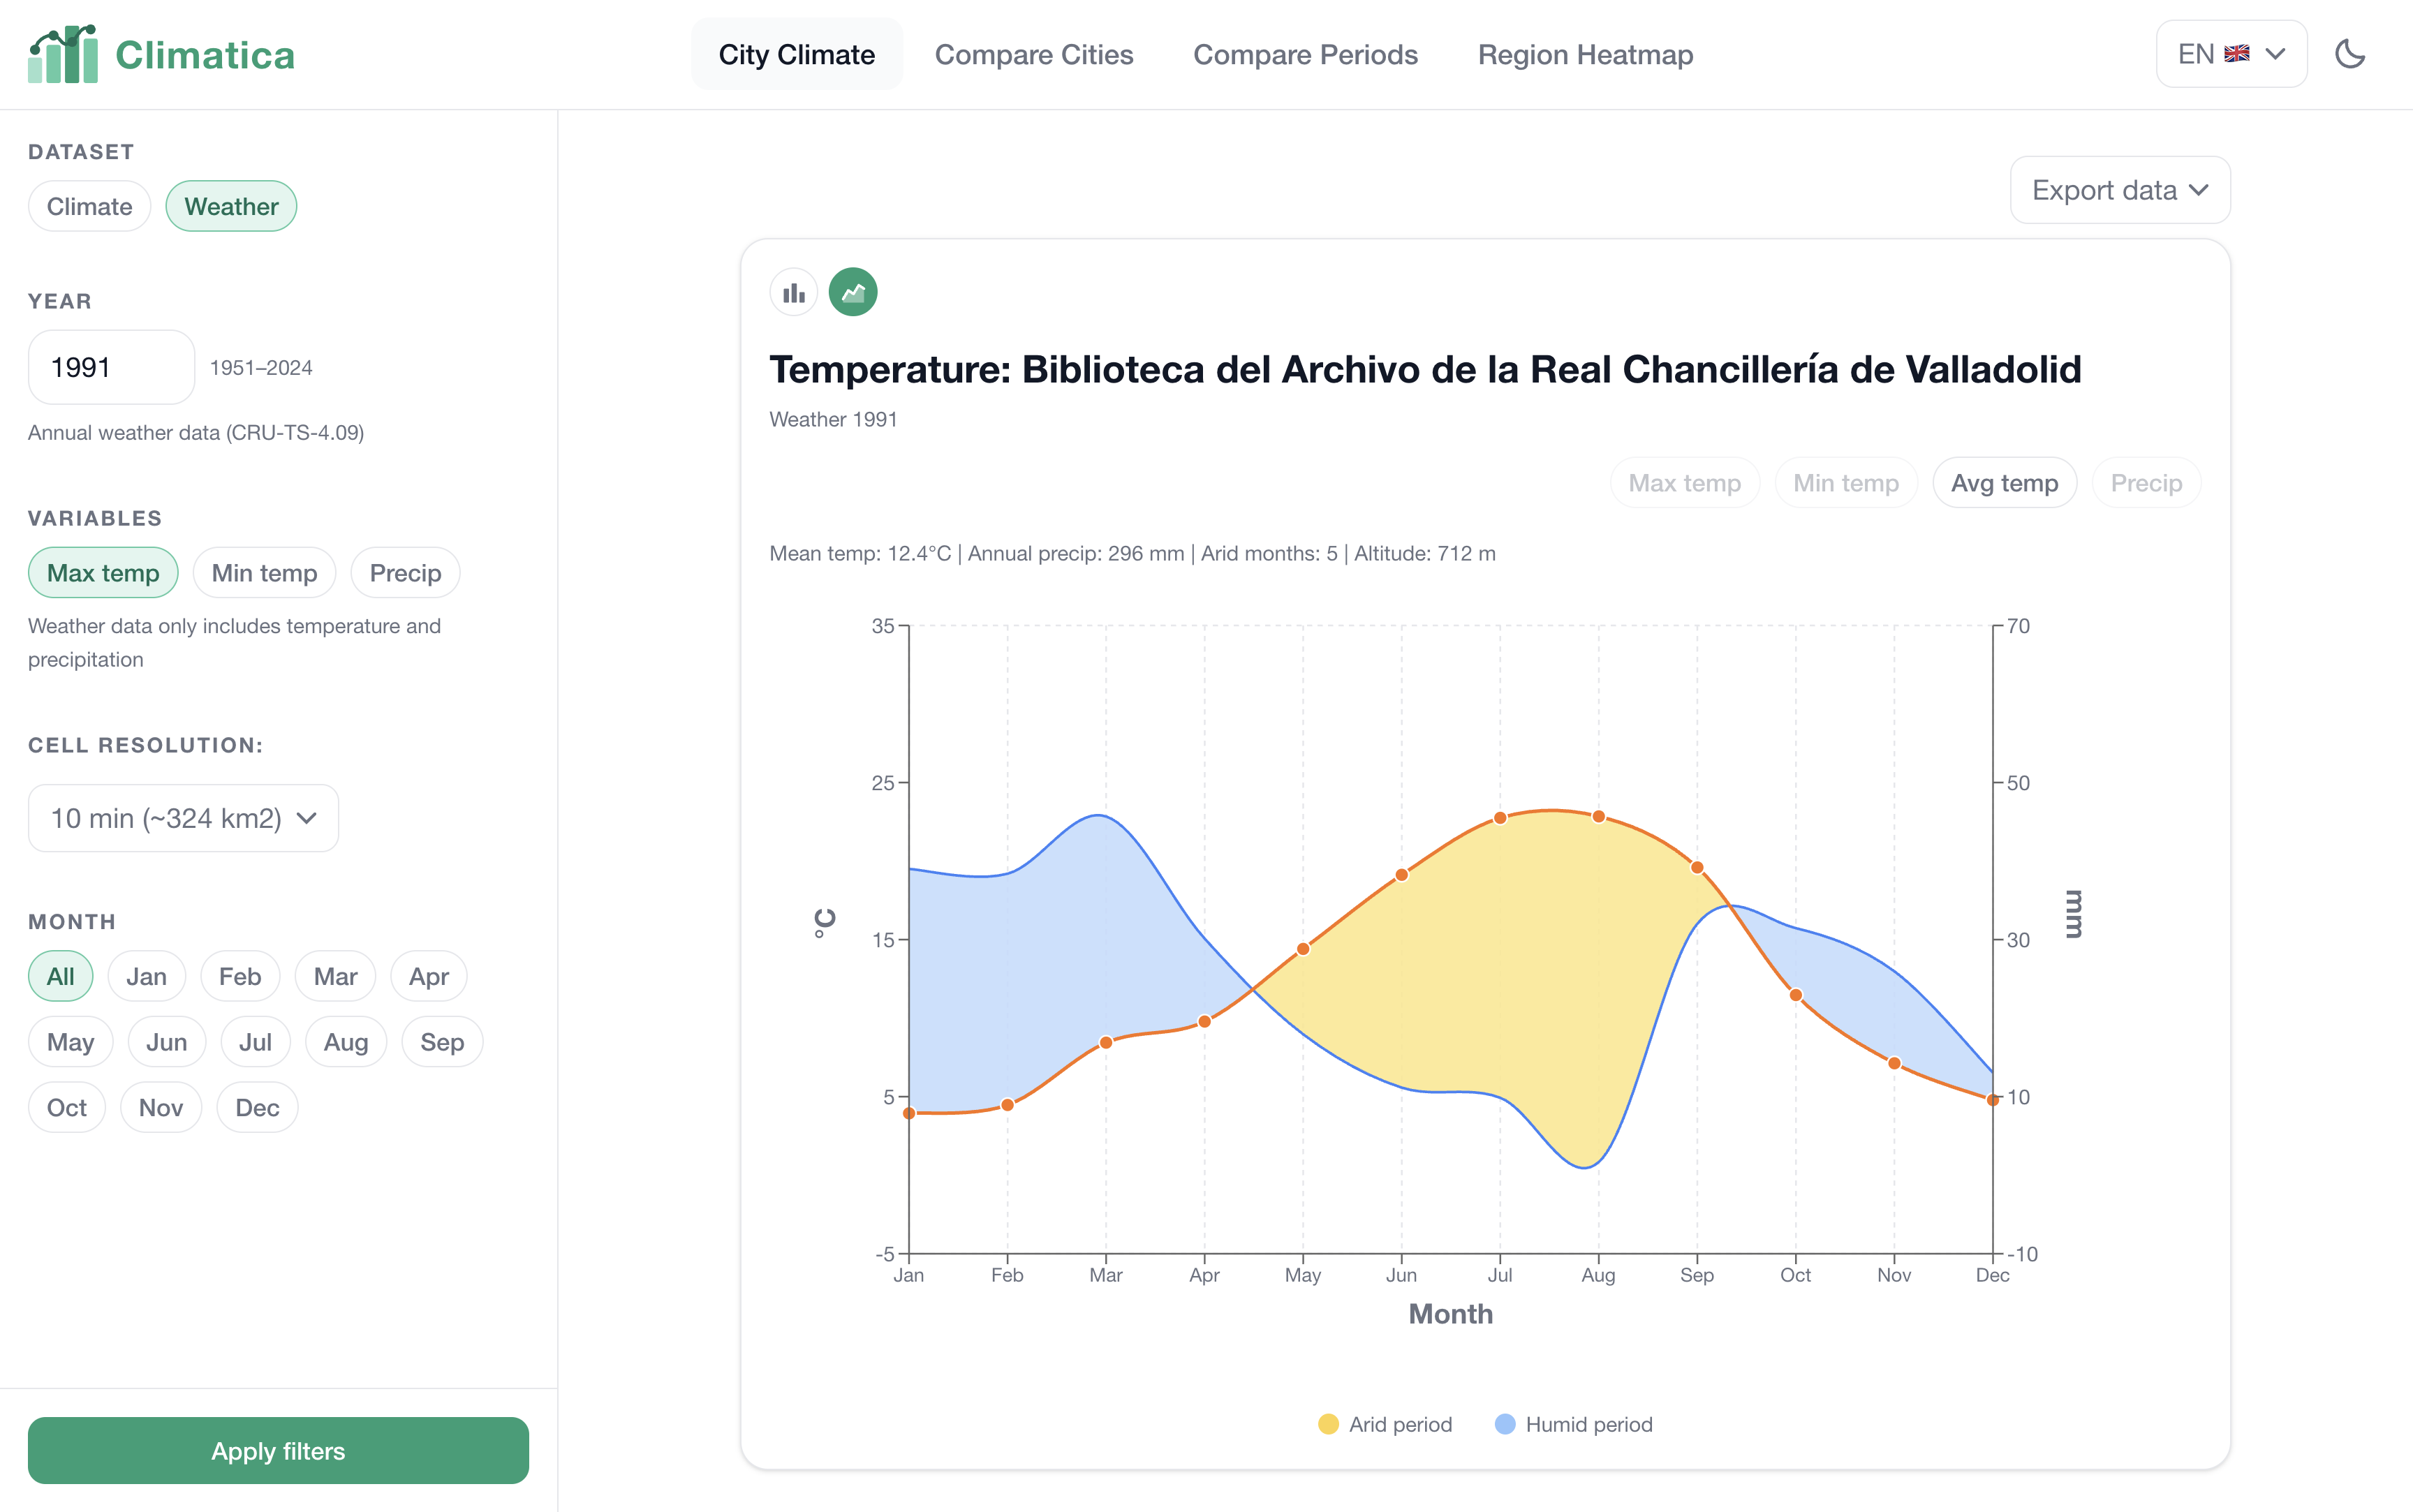
\includegraphics[width=0.9\textwidth]{Images/climatica-walter-lieth.png}
  \caption{City Climate page --- Walter-Lieth climatogram for the same city and
    period. Yellow filled areas indicate arid months; blue filled areas indicate
    humid months.}
  \label{fig:page_city_wl}
\end{figure}

Several technical details are worth noting. When the user clicks the map, a
provisional city object with the raw coordinates is committed to state
immediately so that the climate data fetch begins without waiting for Wikidata
reverse geocoding. If the geocoding call returns a named city, the label is
upgraded in place; a ref prevents stale responses from older clicks from
overwriting newer results. The raster cell outline is computed by parsing the
cell IRI returned by SCRAPI: the \texttt{\_r\{row\}c\{col\}} suffix encodes the
row and column indices, from which the bounding box is derived using the known
cell dimensions of the selected grid resolution.

\subsection{Compare Cities}\label{APP_PROTO_COMPARE}

The Compare Cities page (Figure~\ref{fig:page_compare}) allows the user to
select two cities --- identified by green (City~A) and orange (City~B) colour
codes --- and view their climate profiles overlaid on shared axes. The page
displays a colour-coded statistics table and four derived insight cards: warmer
city, city with more rainfall, hottest month, and coldest month. A mini-map in
the top-right corner shows the geographic positions of both cities.

\begin{figure}[H]
  \centering
  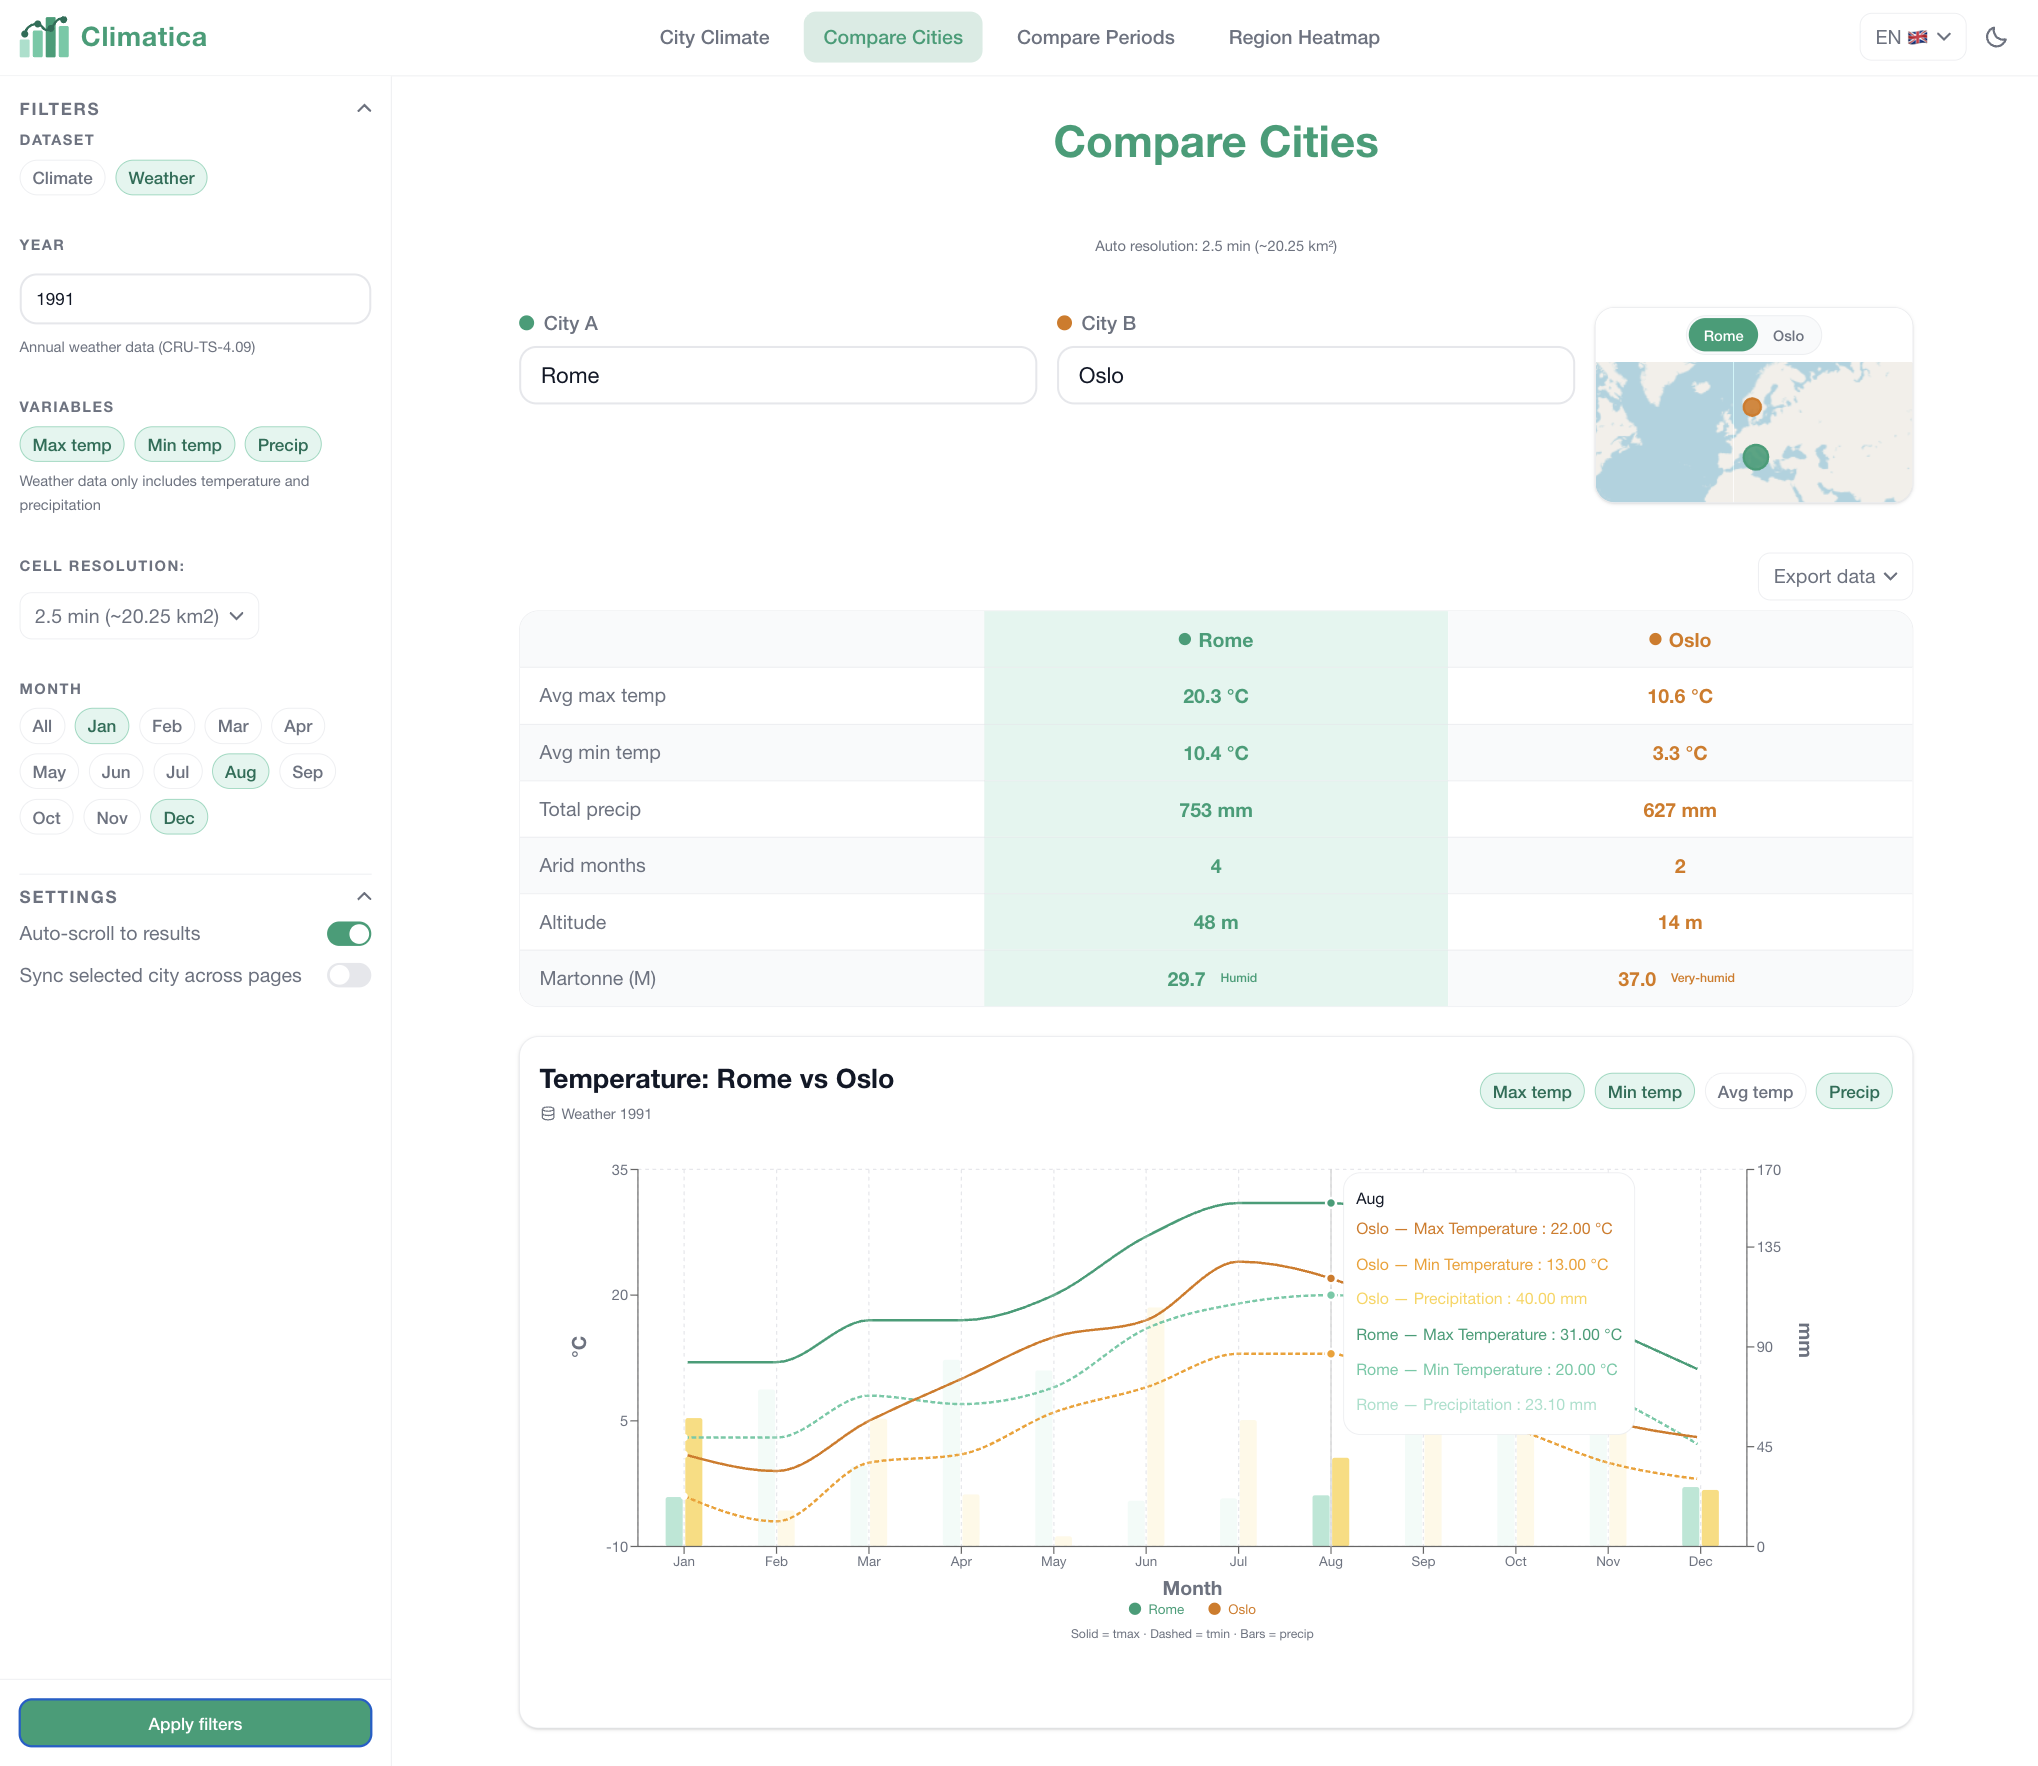
\includegraphics[width=0.9\textwidth]{Images/climatica-compare-cities.png}
  \caption{Compare Cities page comparing Rome and Oslo (weather dataset,
    year~1991). The upper section shows city search fields, a mini-map, and a
    colour-coded statistics table; the lower section shows the overlaid
    temperature and precipitation chart with derived insight cards.}
  \label{fig:page_compare}
\end{figure}

Both cities are fetched in parallel using \texttt{Promise.all} inside a single
TanStack Query entry. City selections are written to URL search parameters,
enabling the comparison to be shared by copying the URL.

\subsection{Compare Periods}\label{APP_PROTO_PERIODS}

The Compare Periods page allows the user to analyse how the climate of a single
city has shifted across time. The page operates in two distinct modes depending
on the active dataset.

\textbf{Climate mode} (Figure~\ref{fig:page_periods_climate}) compares exactly
two 30-year climate normals chosen from the five available periods
(1951--1980, 1961--1990, 1970--2000, 1981--2010, 1991--2020). The two periods
are selected via dropdowns and their monthly data are fetched in parallel via
\texttt{Promise.all} with \texttt{keepPreviousData: true}, so the chart remains
visible while new data loads. Below the overlaid chart, two trend indicator
cards summarise the change: one for maximum temperature and one for total
precipitation. Positive differences are coloured with the Period~B accent colour
and negative differences with Period~A, giving an immediate visual indication of
warming or drying trends.

\textbf{Weather mode} (Figure~\ref{fig:page_periods_weather}) supports between
2 and 5 individual years selected from the CRU-TS-4.09 archive (1951--2024).
Years are managed through the sidebar filter panel (Figure~\ref{fig:page_periods_sidebar})
and persisted to \texttt{localStorage} via a Zustand store. Each selected year
is fetched as a separate parallel TanStack Query (\texttt{useQueries}), and
results accumulate progressively as they arrive --- columns for still-loading
years show skeleton placeholders in the statistics table, making partial results
immediately visible without blocking the entire view. Each year is assigned one
of five fixed colours (green~$\to$~amber~$\to$~blue~$\to$~rose~$\to$~violet),
all overlaid on a single shared chart.

\begin{figure}[H]
  \centering
  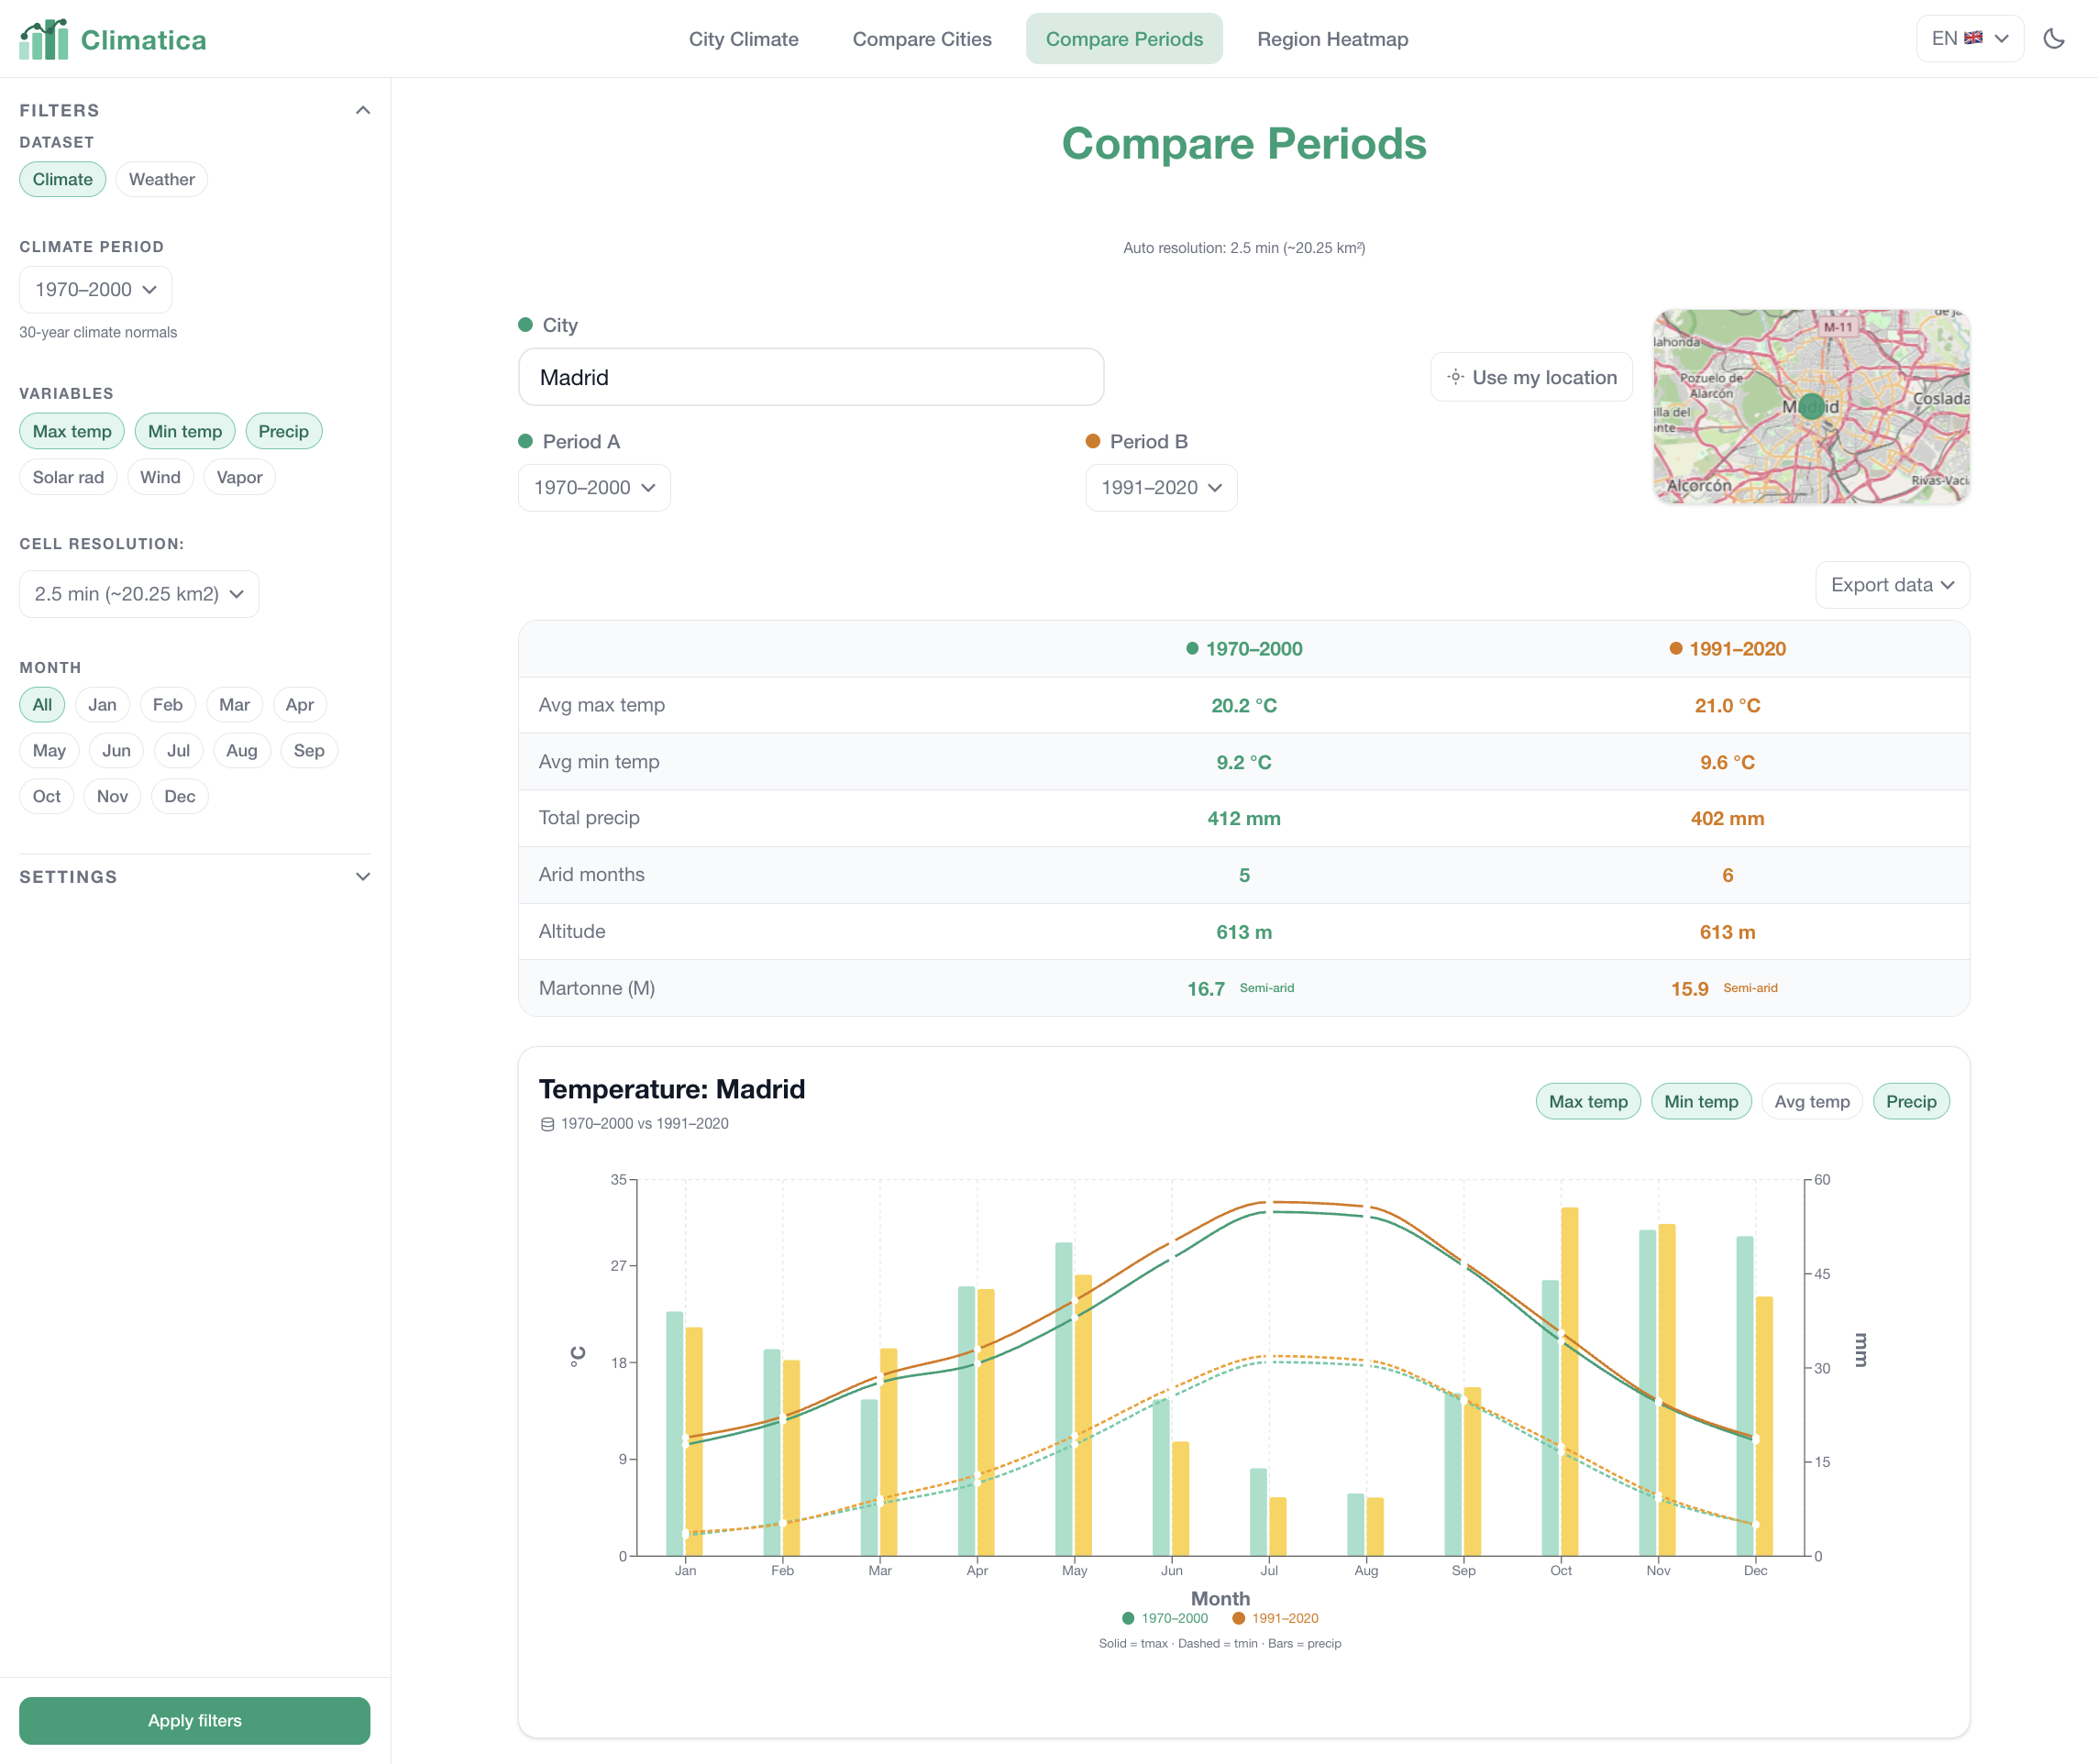
\includegraphics[width=0.9\textwidth]{Images/climatica-compare-periods-climate.png}
  \caption{Compare Periods page --- climate mode for Madrid, comparing the
    1970--2000 and 1991--2020 climate normals. The statistics table shows a
    warming trend (+0.8\,°C avg max) and slight decrease in precipitation
    between the two periods.}
\end{figure}

\begin{figure}[H]
  \centering
  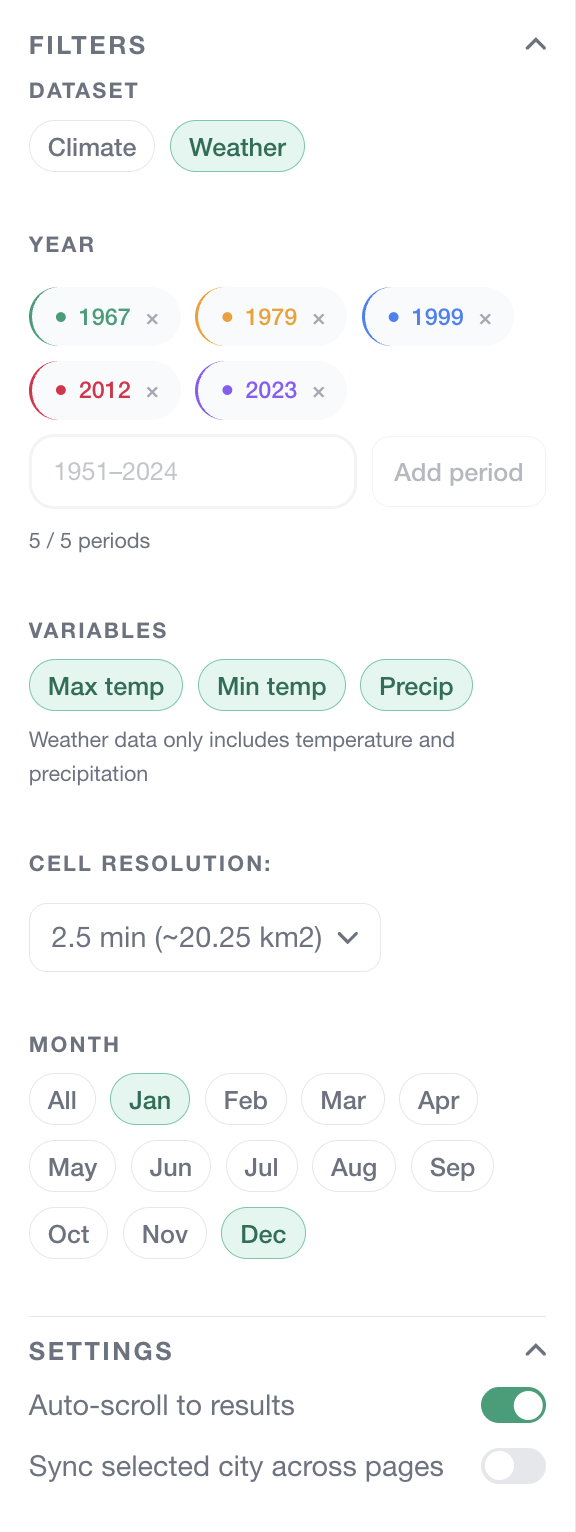
\includegraphics[width=0.5\textwidth]{Images/climatica-compare-periods-sidebar.png}
  \caption{Compare Periods page --- sidebar in weather mode with five years
    selected (1967, 1979, 1999, 2012, 2023). Each year receives a distinct
    colour that carries through to the chart and statistics table. The
    \emph{Add period} input allows adding years up to the maximum of five.
    The Settings section exposes the auto-scroll and city sync toggles.}
  \label{fig:page_periods_sidebar}
\end{figure}

\begin{figure}[H]
  \centering
  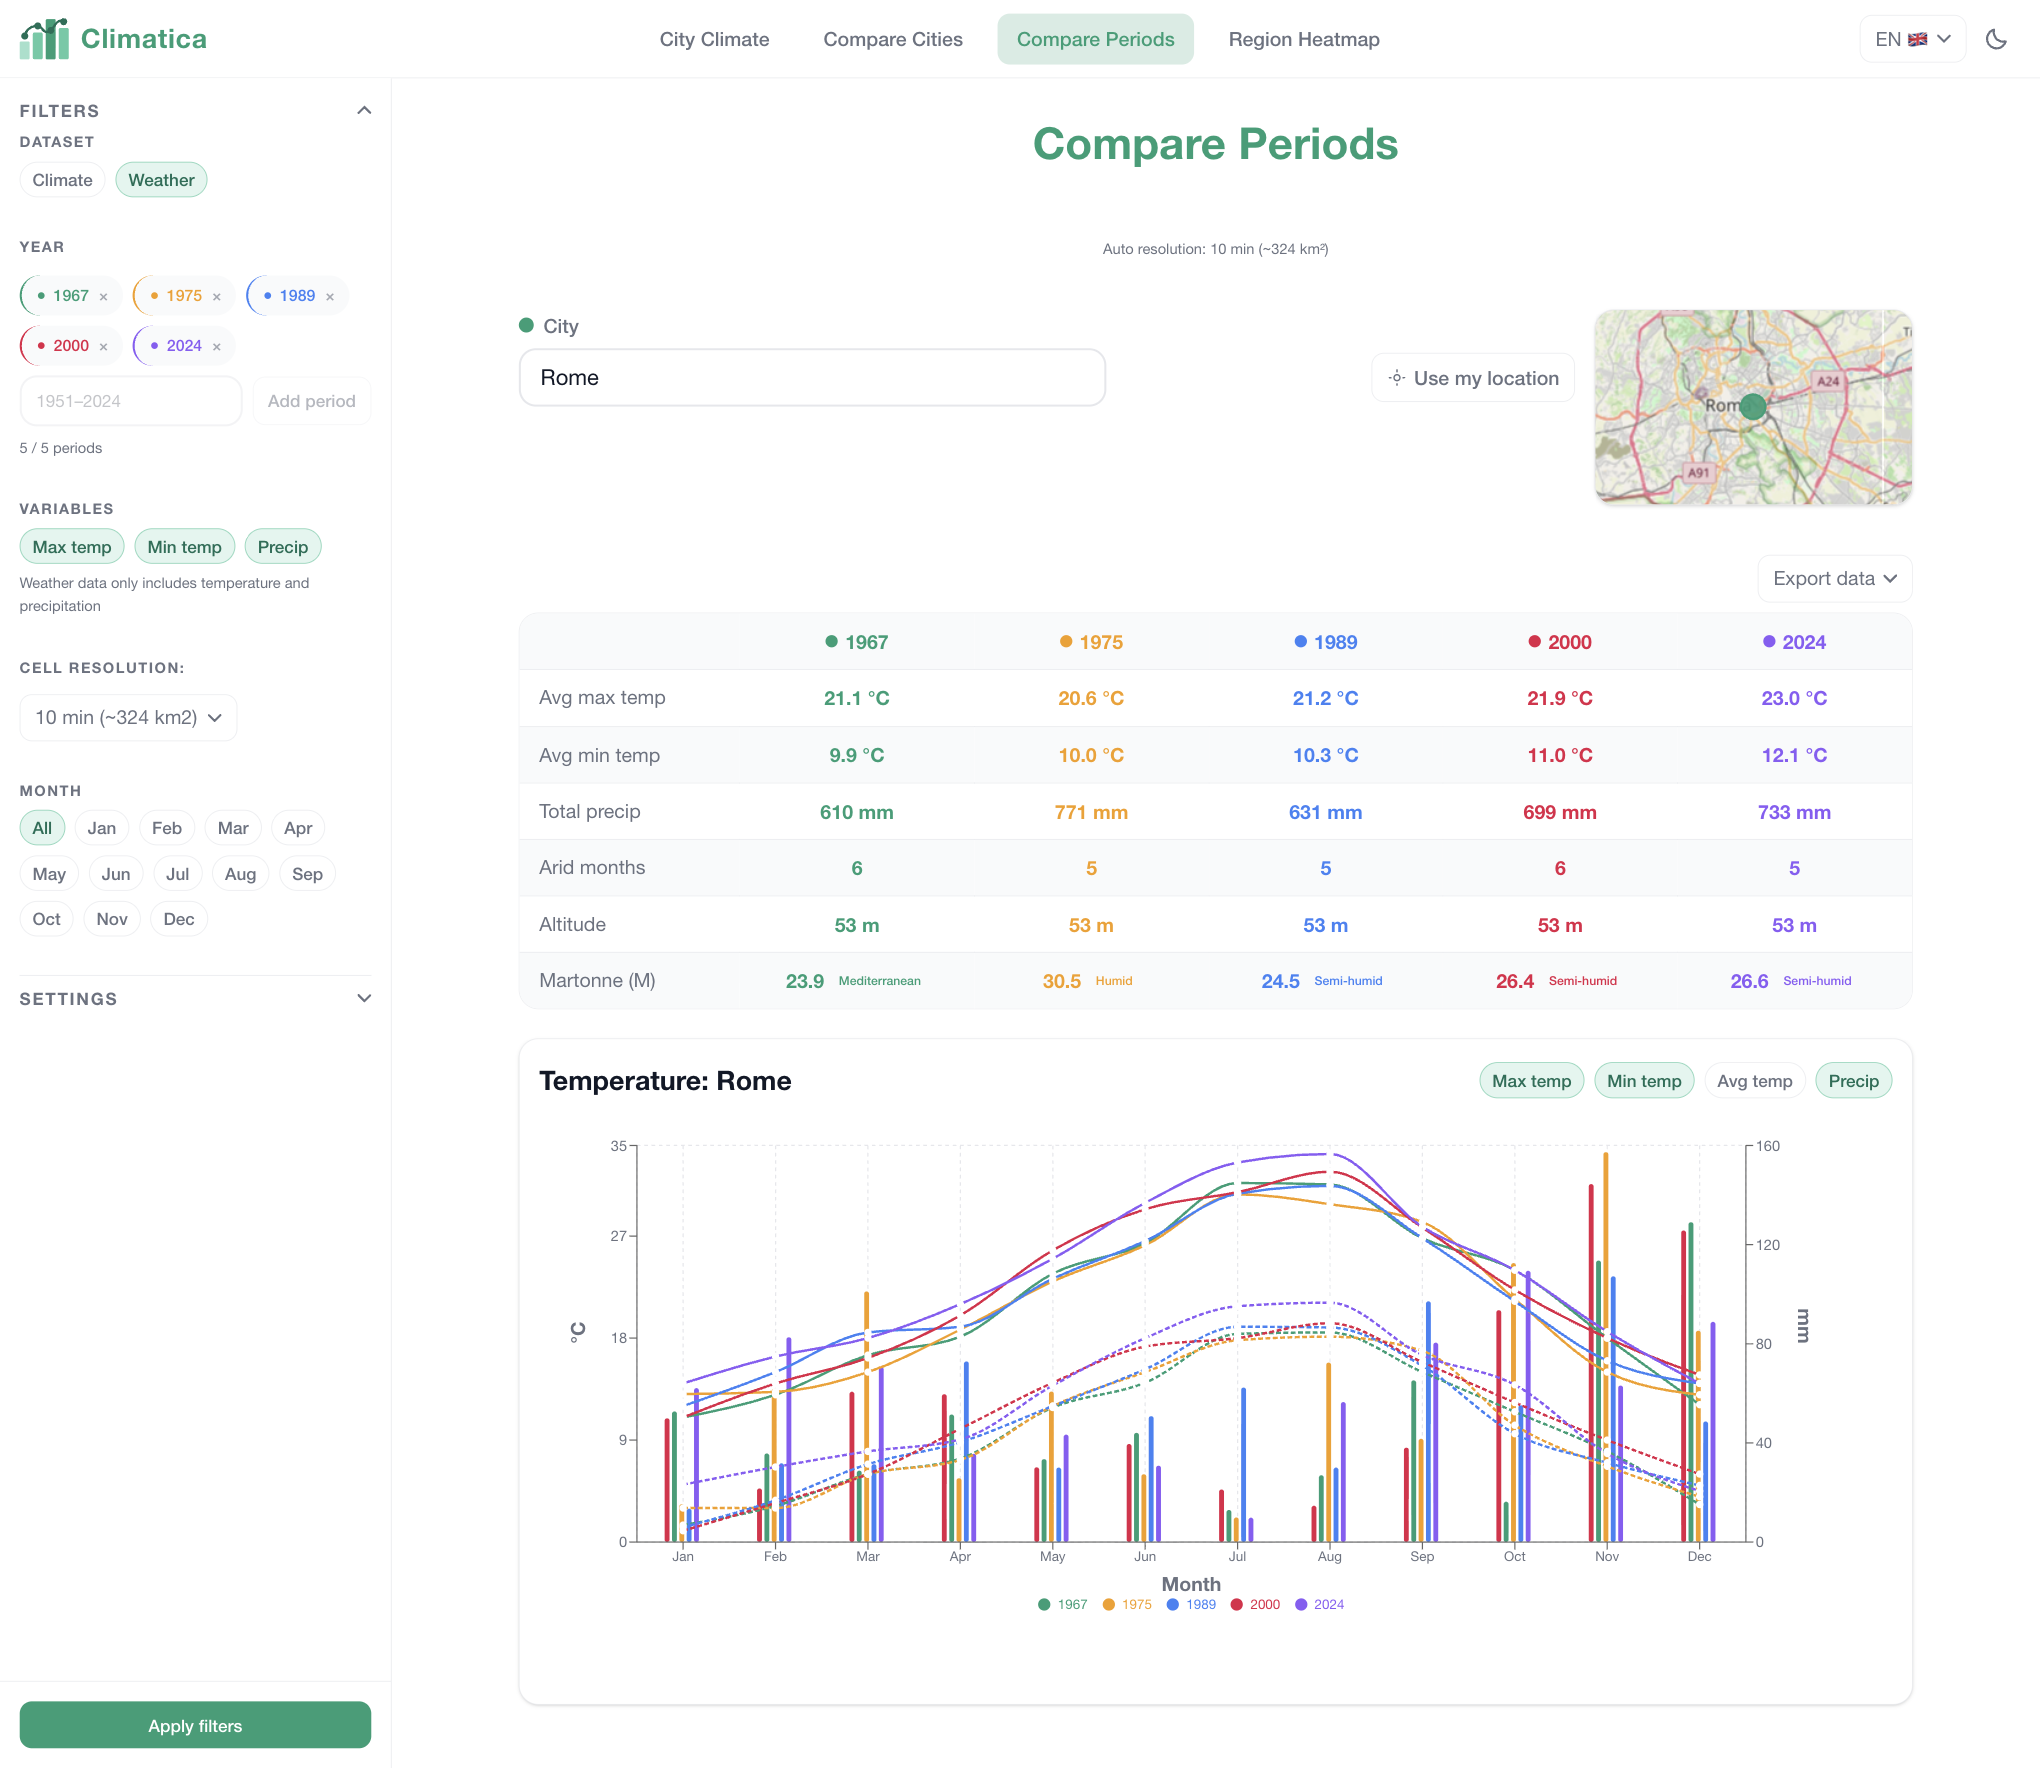
\includegraphics[width=0.9\textwidth]{Images/climatica-compare-periods-weather.png}
  \caption{Compare Periods page --- weather mode with multiple years selected
    simultaneously. Each year is rendered in a distinct colour; the statistics
    table shows one column per year with skeleton placeholders for years still
    loading.}
  \label{fig:page_periods_weather}
\end{figure}

\subsection{Region Heatmap}\label{APP_PROTO_HEATMAP}

The Region Heatmap page allows the user to analyse the spatial distribution of
a climate variable across a geographic region. The user selects a drawing mode
--- bounding box or freeform polygon --- and draws directly on the Leaflet map.
The application then queries all WorldClim raster pixels within the selection
and renders each pixel as a coloured rectangle, forming a spatially resolved
heatmap.

\textbf{Selection modes.} The drawing mode is represented as a discriminated
type with three states: \texttt{"none"}, \texttt{"bbox"}, and
\texttt{"polygon"}. Only one mode is active at a time; switching clears the
opposite selection. The bounding box drawer disables map dragging during
interaction and commits the selection on mouse up. The polygon drawer
accumulates vertices on click; when three or more vertices exist and the cursor
comes within 14 pixels of the first vertex, a snap indicator appears and the
next click closes the polygon. Both selections are persisted in URL search
parameters for shareability.

\textbf{Data fetching.} Two hooks handle the two selection modes:
\texttt{useGetHeatmapData} for bounding boxes and
\texttt{useGetHeatmapPolygonData} for polygons. Each hook fires a single
TanStack Query whose \texttt{queryFn} issues two SCRAPI requests in a
\texttt{Promise.all}: one for the per-pixel grid and one for the area-average
summary shown in the regional profile panel. The inactive hook is disabled
automatically because its input is \texttt{null}.

\textbf{Pixel rendering.} Pixels are rendered as SVG-backed
\texttt{L.rectangle} overlays managed by a single \texttt{L.layerGroup}. On
every relevant state change, the group is cleared and rebuilt. The geographic
position of each rectangle is computed from the pixel IRI returned by SCRAPI:
the \texttt{\_r\{row\}c\{col\}} suffix is parsed to recover the row and column
index, from which the cell bounding box is derived as
$\mathit{north} = 90 - \mathit{row} \times \mathit{cellSize}$ and
$\mathit{west} = -180 + \mathit{col} \times \mathit{cellSize}$. This avoids
any dependency on explicit latitude/longitude fields, which are absent for
water cells.

\textbf{Colour scale.} The normalisation formula is
$t = (\mathit{value} - \mathit{min}) / (\mathit{max} - \mathit{min})$, where
\textit{min} and \textit{max} are the observed extremes in the current response.
Two palettes are available: a nine-stop RdYlBu diverging palette for temperature
(blue cold $\to$ red hot) and a four-stop sequential brown palette for
precipitation. The legend bar samples the colour function at ten evenly spaced
positions and renders a CSS \texttt{linear-gradient}.

\begin{figure}[H]
  \centering
  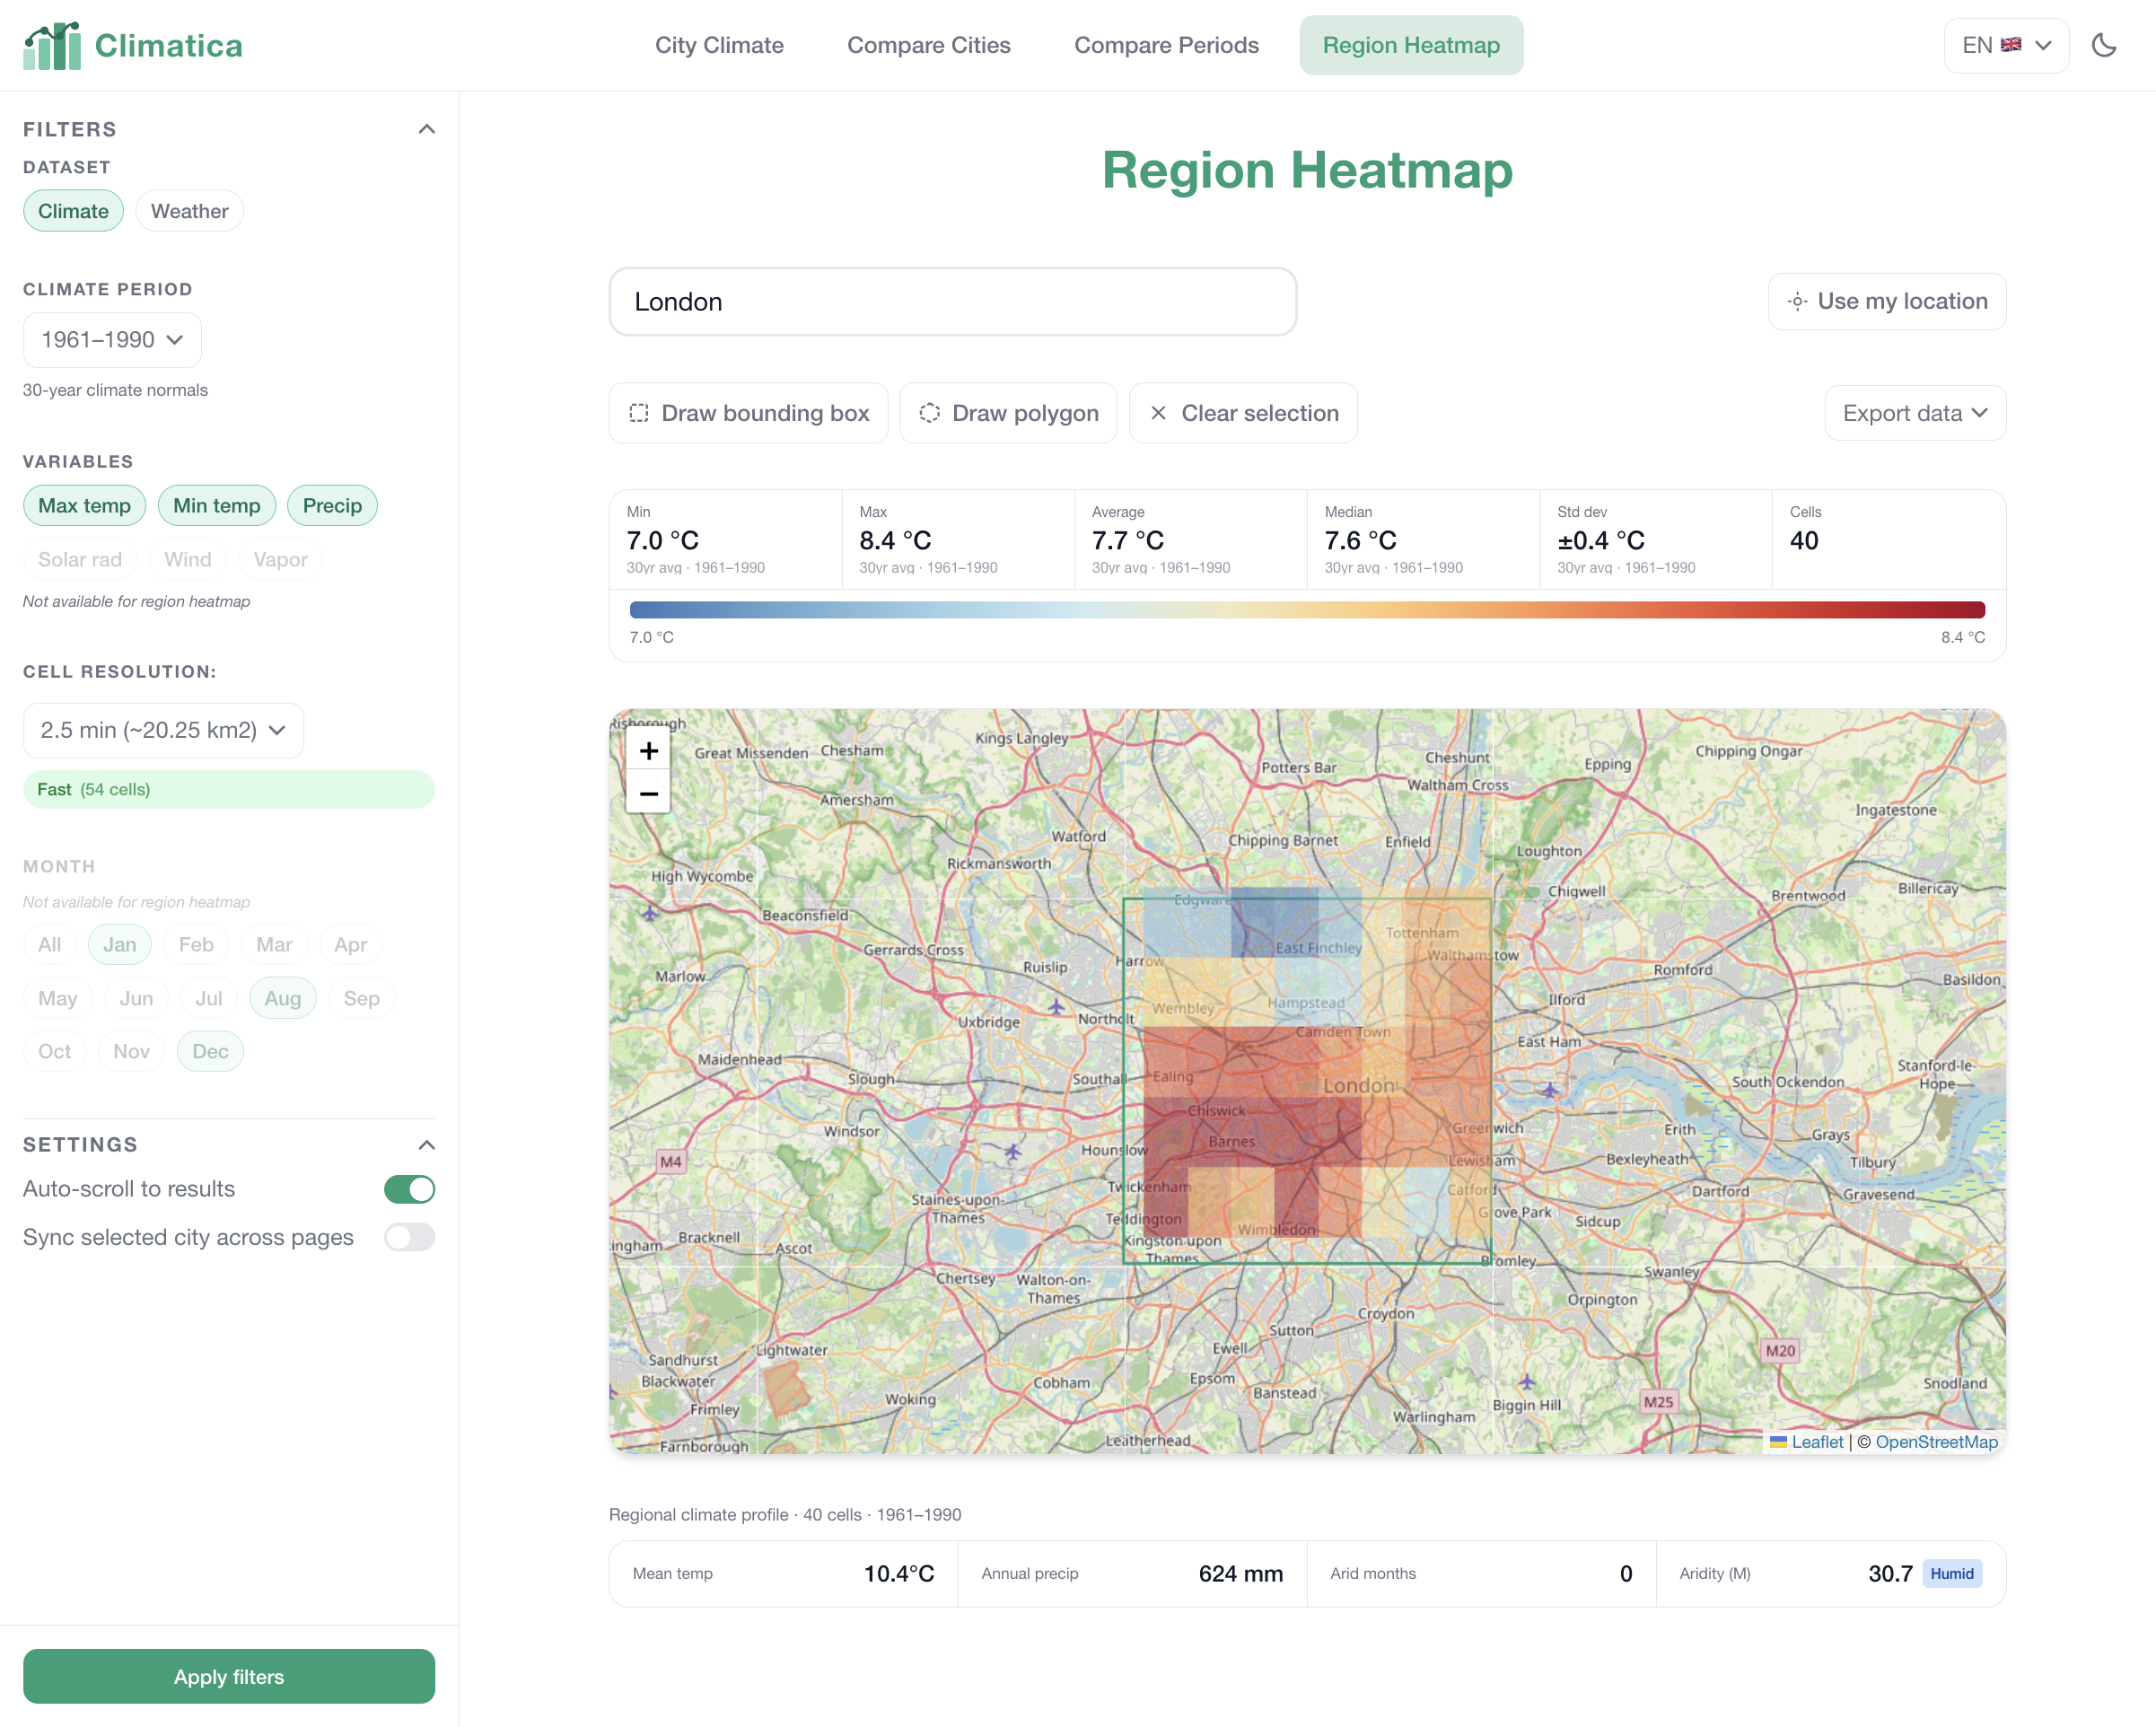
\includegraphics[width=0.9\textwidth]{Images/climatica-heatmap-bbox.png}
  \caption{Region Heatmap page --- bounding box selection over Greater London
    (climate dataset, 1961--1990, maximum temperature). The colour scale runs
    from blue (7.0\,°C) to red (8.4\,°C); the regional profile below the map
    summarises the 40 queried cells with mean temperature, annual precipitation,
    arid months, and the Martonne aridity index.}
  \label{fig:page_heatmap_bbox}
\end{figure}

\begin{figure}[H]
  \centering
  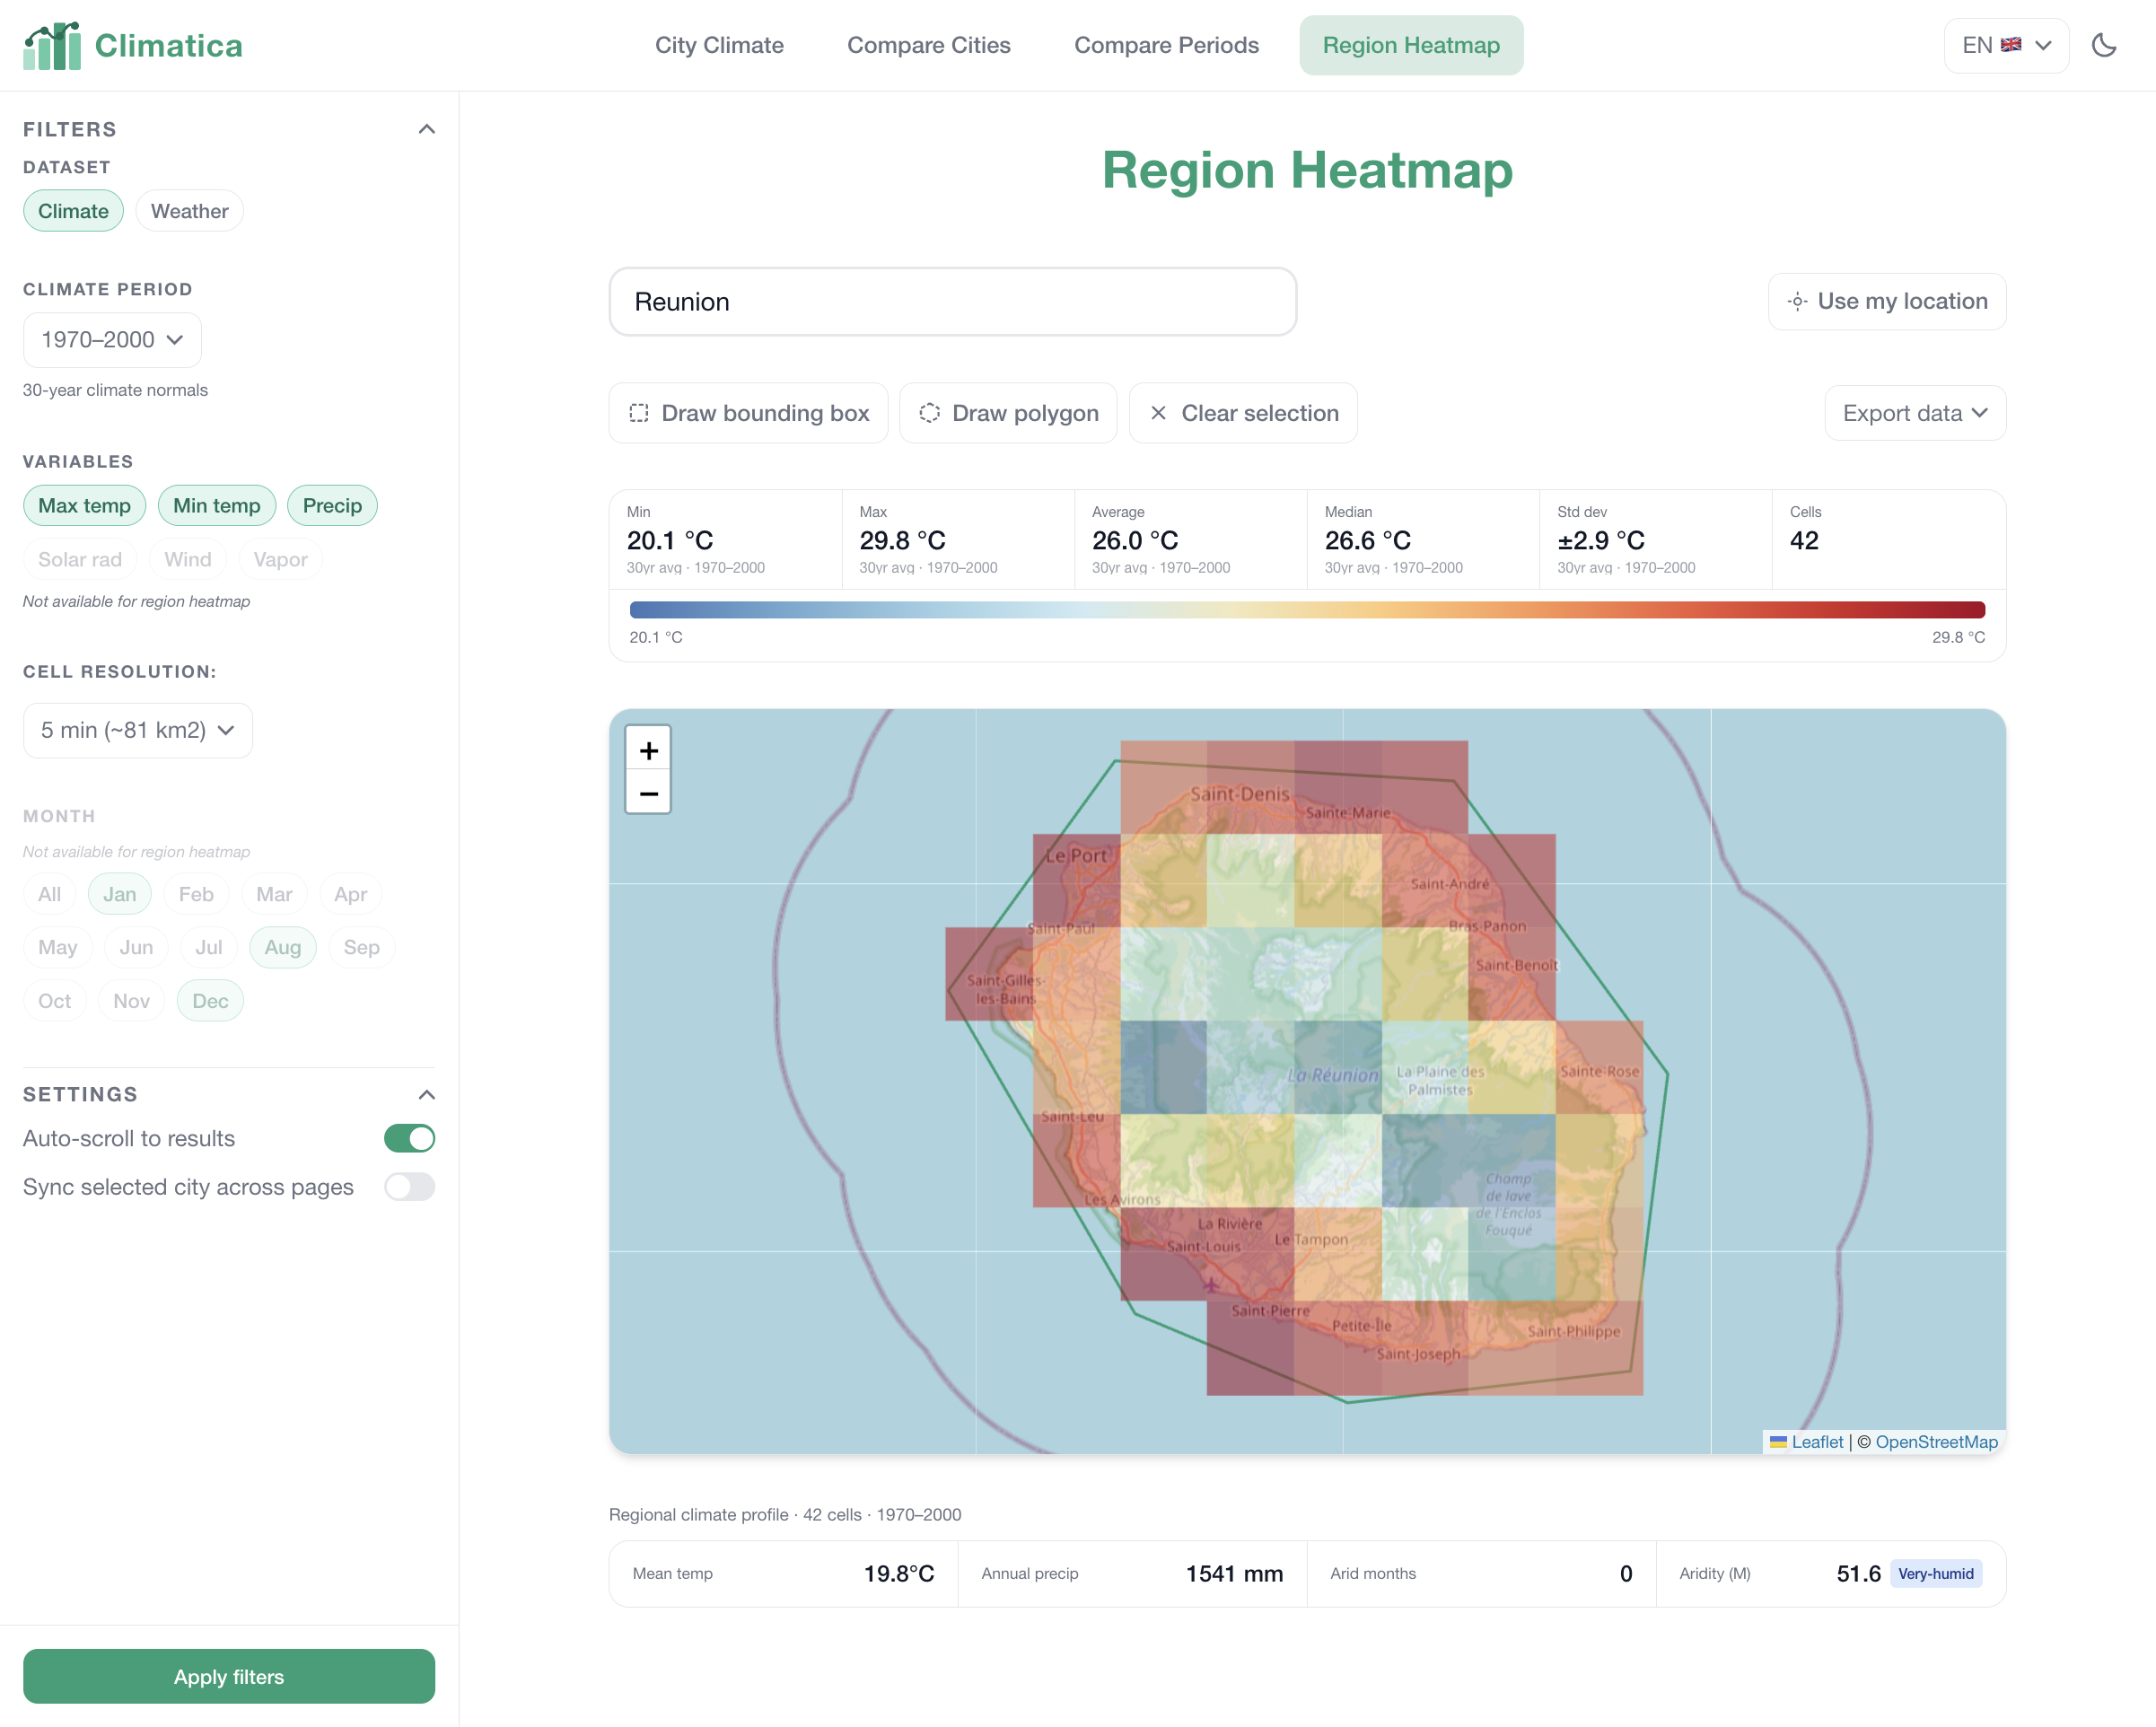
\includegraphics[width=0.9\textwidth]{Images/climatica-heatmap-polygon.png}
  \caption{Region Heatmap page --- freeform polygon selection over the island
    of Réunion (climate dataset, 1970--2000, maximum temperature). The polygon
    boundary is drawn by the user vertex by vertex; the application queries all
    42 raster cells whose centroids fall within the polygon. The wide
    temperature range (20.1--29.8\,°C) reflects the island's significant
    elevation gradient from coastal lowlands to the volcanic highlands.}
  \label{fig:page_heatmap_polygon}
\end{figure}


















% ─── CHAPTER 4 ────────────────────────────────────────────────────────────────
\chapter{Evaluation}\label{EVAL}

This chapter presents the evaluation of Climatica. Section~\ref{EVAL_METHOD}
describes the evaluation methodology and the study design.
Section~\ref{EVAL_PARTICIPANTS} profiles the participants. Section~\ref{EVAL_SUS}
reports the usability results derived from the System Usability Scale.
Section~\ref{EVAL_QUAL} analyses the open-ended feedback.
Section~\ref{EVAL_DEMO} presents a representative usage scenario.
Section~\ref{EVAL_DISCUSS} discusses the results, acknowledges limitations,
and identifies directions for future work.

% ─── 4.1 Methodology ─────────────────────────────────────────────────────────
\section{Evaluation Methodology}\label{EVAL_METHOD}

The evaluation was conducted as a user study on 3 June 2026 during a
presentation session at the Universidad de Valladolid attended by students
from multiple European universities participating in an Erasmus+ programme.
All participants were domain users --- students enrolled in degree programmes
in forestry, environmental science, or biology --- rather than software
professionals, making them representative of Climatica's intended audience.

Each participant was given a brief live demonstration of the application and
then invited to explore it independently on their own device for approximately
ten minutes. At the end of the session they were asked to complete an online
questionnaire. The questionnaire comprised four parts:

\begin{enumerate}
  \item \textbf{Background questions} --- university, degree programme, year
    of study, and self-assessed knowledge level across six domains (climatology,
    GIS, data analysis, programming, databases, and general IT/web tools).
  \item \textbf{System Usability Scale (SUS)} --- the standard ten-item
    questionnaire~\cite{brooke1996sus} designed to produce a single usability
    score on a 0--100 scale.
  \item \textbf{Net Promoter Score (NPS)} --- a single question asking how
    likely the participant is to recommend Climatica to a friend or colleague,
    rated 0--10.
  \item \textbf{Open-ended questions} --- three free-text fields asking what
    the participant liked least, liked most, and would suggest as an
    improvement.
\end{enumerate}

Participation was voluntary and anonymous. Respondents were asked to confirm
their informed consent before proceeding. All 27 responses collected were
retained for analysis; no responses were excluded.

% ─── 4.2 Participant Profile ─────────────────────────────────────────────────
\section{Participant Profile}\label{EVAL_PARTICIPANTS}

Twenty-seven students from ten European institutions completed the
questionnaire. The institutions represented included the Free University of
Bolzano (Italy), the University of Molise (Italy), the Warsaw University of
Life Sciences (Poland), the University for Sustainable Development Eberswalde
(Germany), and the Polytechnic Institute of Bragança (Portugal), among others.

The distribution across fields of study was strongly weighted towards
Forestry and Natural Resource Management (18 respondents, 67\%), followed by
Biology (6 respondents, 22\%), and Engineering, Earth Sciences, and Forest
Information Technology (one respondent each). The majority of respondents were
in their second or third year of study (13 and 6 respondents respectively).

Table~\ref{tab:knowledge} shows the self-reported knowledge levels across the
six assessed domains, expressed as means on a five-point scale
(0~=~None, 1~=~Basic, 2~=~Intermediate, 3~=~Advanced, 4~=~Expert). The
participant group was moderately experienced in climatology, GIS, and data
analysis --- the domains most directly relevant to Climatica's subject matter
--- but had limited programming and database backgrounds, consistent with a
target audience of domain specialists rather than software developers.

\begin{table}[H]
  \centering
  \caption{Self-reported knowledge levels of study participants
           (mean on a 0--4 scale; $n = 27$).}
  \label{tab:knowledge}
  \small
  \begin{tabular}{lcc}
    \toprule
    \textbf{Domain} & \textbf{Mean} & \textbf{Interpretation} \\
    \midrule
    Climatology and meteorology   & 2.00 & Intermediate \\
    GIS and geospatial data       & 2.22 & Intermediate--Advanced \\
    Data analysis \& visualisation & 2.00 & Intermediate \\
    Programming                    & 1.26 & Basic \\
    Databases                      & 1.37 & Basic--Intermediate \\
    General IT / web tools         & 1.56 & Basic--Intermediate \\
    \bottomrule
  \end{tabular}
  \normalsize
\end{table}

% ─── 4.3 SUS Results ─────────────────────────────────────────────────────────
\section{Usability Results}\label{EVAL_SUS}

\subsection{System Usability Scale}\label{EVAL_SUS_SCORE}

The System Usability Scale (SUS) is a ten-item Likert questionnaire in which
alternating items are positively and negatively worded. The raw score for each
respondent is computed as:

\[
  \text{SUS} = 2.5 \times \left[
    \sum_{i \in \text{odd}} (x_i - 1)
    + \sum_{i \in \text{even}} (5 - x_i)
  \right]
\]

where $x_i$ is the respondent's rating for item $i$ on a 1--5 scale. The
resulting score lies in the range $[0, 100]$.

The mean SUS score across all 27 respondents was \textbf{84.6} (median~90.0,
standard deviation~14.7, range~47.5--100.0). According to the adjective
rating scale proposed by Bangor et al.~\cite{bangor2009sus}, a score in the
range 80--90 is rated \emph{Excellent} and a score above 90 is rated
\emph{Best Imaginable}. Climatica's mean score of 84.6 therefore falls in the
\emph{Excellent} range and exceeds the widely cited industry average of
68~\cite{brooke1996sus}.

Table~\ref{tab:sus_dist} groups the individual scores by grade band using the
curved grading system of Sauro and Lewis~\cite{sauro2012sus}. Nineteen of the
27 respondents (70\%) awarded a score of 87.5 or higher, placing Climatica in
the A or A+ band for the majority of users. Three respondents (11\%) gave
scores below 65, suggesting that a minority of users encountered meaningful
usability barriers.

\begin{table}[H]
  \centering
  \caption{Distribution of individual SUS scores by grade band ($n = 27$).}
  \label{tab:sus_dist}
  \small
  \begin{tabular}{cclc}
    \toprule
    \textbf{Grade} & \textbf{Score range} & \textbf{Adjective} & \textbf{Count} \\
    \midrule
    A+ & $\geq 84.1$ & Best imaginable & 19 \\
    A  & 80.8--84.0  & Excellent       & 1  \\
    B  & 74.0--80.7  & Good            & 3  \\
    C  & 68.0--73.9  & OK              & 2  \\
    D  & 51.0--67.9  & Poor            & 0  \\
    F  & $< 51.0$    & Awful           & 2  \\
    \bottomrule
  \end{tabular}
  \normalsize
\end{table}

\subsection{Net Promoter Score}\label{EVAL_NPS}

The Net Promoter Score (NPS) question asked participants to rate, on a 0--10
scale, how likely they were to recommend Climatica to a friend or colleague.
Respondents scoring 9--10 are classified as \emph{promoters}, those scoring
7--8 as \emph{passives}, and those scoring 0--6 as \emph{detractors}. The NPS
is then computed as:

\[
  \text{NPS} = \frac{\text{promoters} - \text{detractors}}{n} \times 100
\]

Of the 27 respondents, 15 were promoters (9--10), 9 were passives (7--8), and
3 were detractors (0--6), yielding a mean recommendation score of 8.8 and an
NPS of \textbf{+44}. An NPS above 0 indicates that promoters outnumber
detractors; scores above 30 are generally considered good, and scores above 70
are considered excellent~\cite{reichheld2003nps}. Climatica's score of +44
therefore indicates a strong recommendation intent among the participant group.

% ─── 4.4 Qualitative Feedback ────────────────────────────────────────────────
\section{Qualitative Feedback}\label{EVAL_QUAL}

\subsection{What Participants Liked Most}\label{EVAL_QUAL_LIKED}

The open-ended responses were analysed thematically. The most frequently
recurring theme across the 23 responses to the ``liked most'' question was
\textbf{ease of use and intuitiveness}. Representative comments included:
``I found it very straightforward to use and it provides very useful and
interesting data extremely fast''; ``I like how intuitive it is''; and
``Very easy to use, you can get a lot of information out of it.'' This theme
appeared in approximately 80\% of responses, suggesting that the zero-friction
design goal described in Section~\ref{APP_REQ_NONFUNC} was successfully
perceived by users.

The second most prominent theme was \textbf{global data coverage and
accessibility}. Several respondents highlighted the fact that climate data was
available for any point on the globe without requiring registration or local
software: ``I found it very easy to use and I also like the fact that data is
in raster so you can have it at every point of the globe''; ``Access to data
for any place in the world, fast results, visualisation of climographs and
heatmaps.''

A third theme was \textbf{the comparative and temporal views}. Multiple
respondents specifically mentioned the city comparison and period comparison
features as highlights: ``Comparison, having good visualisation of dataset'';
``The ability to analyse historical climate data and compare it with current
data allows us to understand and assess climate change.''

\subsection{What Participants Liked Least}\label{EVAL_QUAL_DISLIKED}

Nineteen respondents answered the ``liked least'' question. The most commonly
reported issue was \textbf{the PNG export alignment bug}: several respondents
from different devices (Windows PC, iPad) noted that text and chart elements
appeared shifted in exported PNG files relative to their on-screen positions.
This is a known limitation of the \texttt{html2canvas} library used for
rasterisation, which does not perfectly replicate all CSS transformations.

The second reported concern was \textbf{the manual filter application step}.
Two respondents noted that they had to click ``Apply filters'' after changing
filter values, which felt unintuitive: ``You have to click on Apply filters
again''; ``Auto-apply filters when clicking on them.'' This is a deliberate
design decision --- the draft filter pattern described in
Section~\ref{APP_ARCH_DRAFT} prevents expensive API calls from firing on every
individual filter change --- but the tradeoff was not immediately obvious to
all users.

Two respondents mentioned \textbf{heatmap loading performance} as a concern.
The heatmap page queries potentially thousands of pixel values from SCRAPI
and renders them as individual map overlays; at coarse resolutions this is fast,
but finer resolutions over large bounding boxes can take several seconds.

One technically sophisticated respondent raised the absence of \textbf{raw
data download}: ``I like least that Climatica doesn't show raw data or let you
download it easily. Great visuals, but limited access to the underlying
numbers.'' Currently Climatica supports CSV and PNG export of chart data but
does not expose the raw SCRAPI response or the pixel value matrix.

\subsection{Suggested Improvements}\label{EVAL_QUAL_SUGGEST}

The most frequently requested improvement was \textbf{better export
functionality}: fixing the PNG alignment issue, adding SVG export reliability
across platforms, and providing raw data downloads. Several respondents also
requested \textbf{finer-grained time periods} --- specifically, 10-year climate
normals in addition to the existing 30-year normals, and non-overlapping
periods. One respondent suggested a \textbf{mobile application}, and another
asked for \textbf{additional language support} beyond the current three locales.

% ─── 4.5 Demo Scenario ───────────────────────────────────────────────────────
\section{Demo Scenario}\label{EVAL_DEMO}

This section demonstrates Climatica through two representative usage scenarios
drawn from forest management practice, as suggested by the project supervisor.
Both scenarios involve non-specialist users --- forest managers and ecologists
--- who need to interpret historical climate data to support practical decisions
but do not have the GIS or programming background required to query WorldClim
directly.

\subsection{Scenario 1: Updating a Forest Management Plan}\label{EVAL_DEMO_FMP}

\subsubsection{Context}

Forest management plans (FMPs) traditionally incorporate an assessment of the
local climate over the preceding 30-year period. This baseline informs
decisions about species selection: which tree species are appropriate for a
given site is determined in part by the temperature range, precipitation
regime, and aridity of that location. Under a stable climate, a plan valid
today would remain valid for the life of the forest stand.

Climate change has disrupted this assumption. Mean temperatures across the
Iberian Peninsula have risen by approximately 1.5\,$^\circ$C over the past
50 years~\cite{ipcc2021}, and precipitation has become more variable and
increasingly concentrated in fewer, more intense events. A species that was
well-suited to a site under the 1961--1990 climate normal may be under
stress --- or near the edge of its physiological tolerance --- under the
1991--2020 normal. A forest manager updating an FMP for a stand in Castilla
y Le\'{o}n therefore needs to understand not only the current climate of the
site but also how it has shifted over the past three decades.

\subsubsection{Step 1: City Climate Profile}

The manager opens Climatica and searches for \textbf{Valladolid}, the
administrative centre of the region and the nearest city to many of the
managed stands. The City Climate page loads the climate profile for the
1991--2020 climate normal (Figure~\ref{fig:demo_fmp_city}), showing an average
maximum temperature of 19.3\,$^\circ$C, average minimum temperature of
7.1\,$^\circ$C, total annual precipitation of 420\,mm, altitude of 699\,m,
and four arid months. The Martonne aridity index of 18.1 places the site in
the \emph{Semi-arid} category.

The Walter-Lieth climatogram makes the seasonal water deficit immediately
visible: the yellow arid area spans four summer months, confirming that the
site operates close to the physiological tolerance limits of moisture-demanding
species. This is the baseline against which the manager will assess whether the
current species composition --- predominantly \textit{Pinus pinea} and
\textit{Quercus ilex} --- remains appropriate.

\begin{figure}[H]
  \centering
  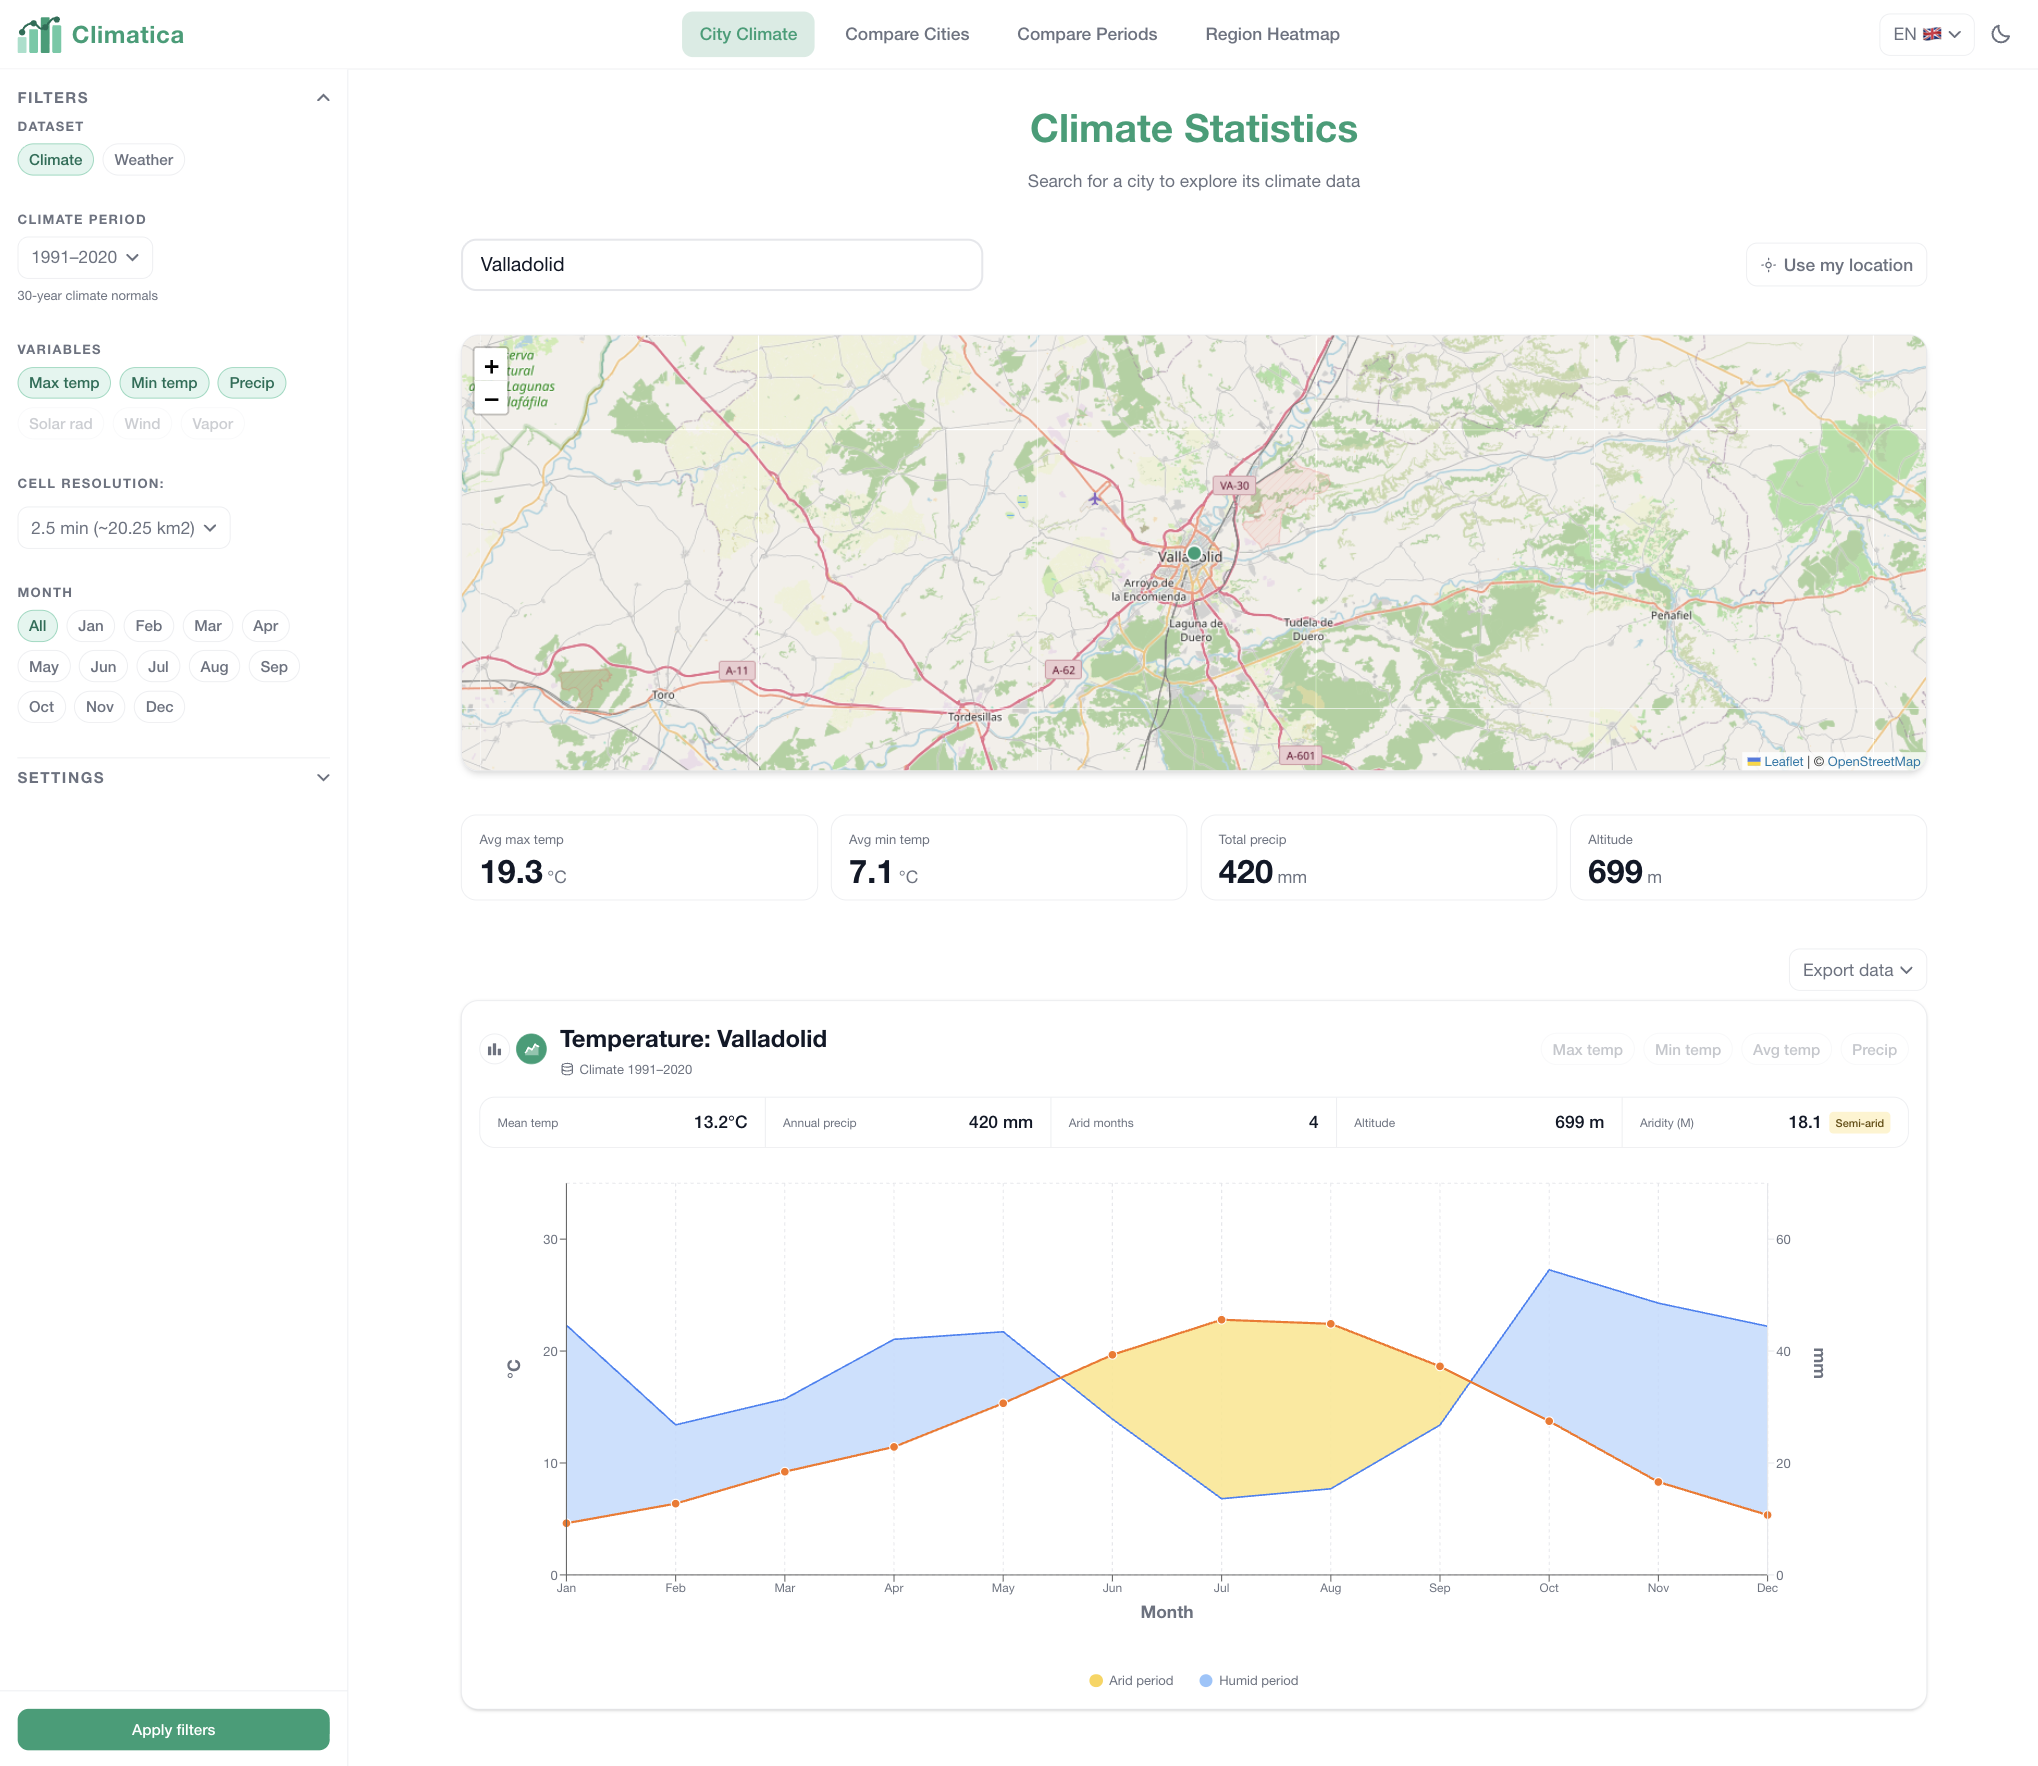
\includegraphics[width=0.9\textwidth]{Images/climatica-demo-fmp-city-climate.png}
  \caption{City Climate page for Valladolid (climate dataset, 1991--2020
    normal). The Walter-Lieth climatogram shows four arid summer months
    (yellow area). The stat cards confirm an average maximum temperature of
    19.3\,$^\circ$C, total annual precipitation of 420\,mm, and a Martonne
    aridity index of 18.1 (Semi-arid).}
  \label{fig:demo_fmp_city}
\end{figure}

\subsubsection{Step 2: Detecting the Climate Shift}

The manager switches to the \textbf{Compare Periods} page and selects
Valladolid with the Climate dataset, setting Period~A to 1961--1990 and
Period~B to 1991--2020 (Figure~\ref{fig:demo_fmp_periods}). The statistics
table and overlaid chart immediately reveal the direction and magnitude of
the change: average maximum temperature increased by \textbf{+1.0\,$^\circ$C}
(from 18.3\,$^\circ$C to 19.3\,$^\circ$C), average minimum temperature
increased by +0.6\,$^\circ$C, and total annual precipitation decreased by
\textbf{11\,mm} (from 431\,mm to 420\,mm). The number of arid months
increased from 4 to 5, meaning that one additional month crossed the aridity
threshold in the more recent normal. The Martonne aridity index dropped from
19.3 to 18.1, remaining in the Semi-arid category but moving further from the
boundary with the less arid class.

The trend indicator cards at the bottom of the page make these changes
immediately legible: \textbf{+1.0\,$^\circ$C} temperature increase and
\textbf{$-$12\,mm} precipitation decrease between the two periods. The manager
records these figures in the FMP as evidence of an ongoing warming and drying
trend consistent with regional climate projections.

\begin{figure}[H]
  \centering
  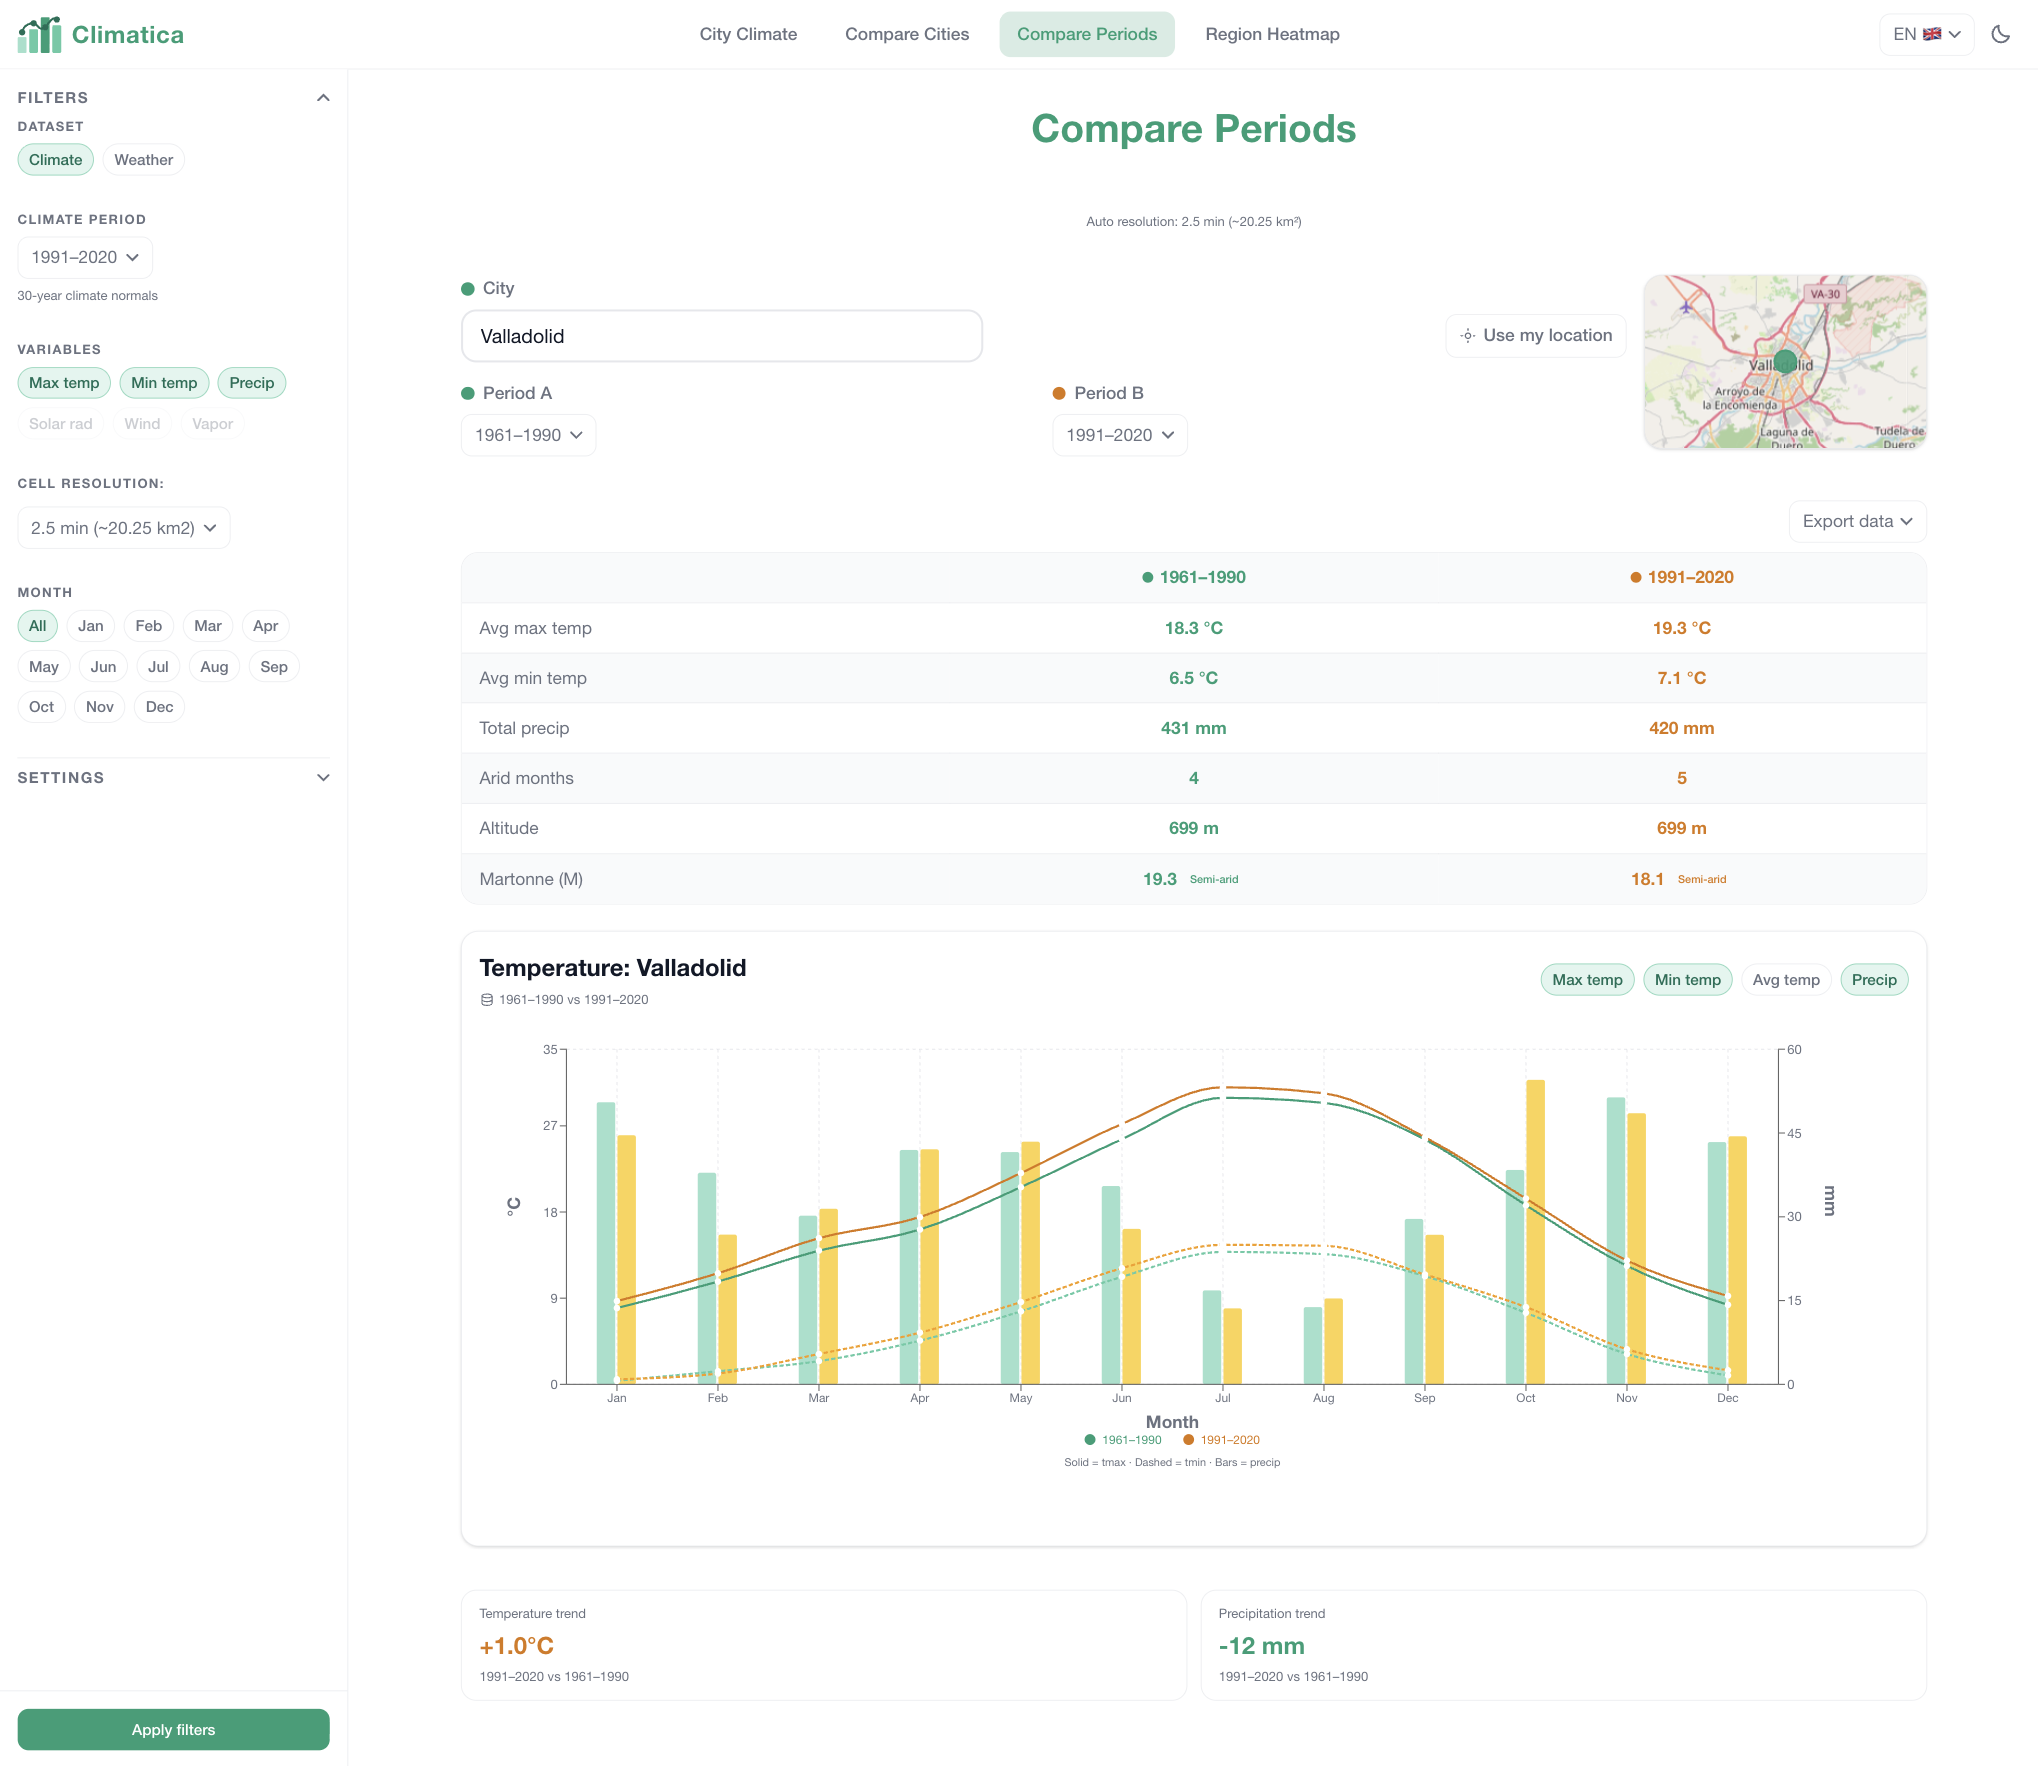
\includegraphics[width=0.9\textwidth]{Images/climatica-demo-fmp-compare-periods.png}
  \caption{Compare Periods page for Valladolid comparing the 1961--1990 and
    1991--2020 climate normals. The statistics table shows a +1.0\,$^\circ$C
    increase in average maximum temperature and a decrease of 11\,mm in total
    precipitation. The trend indicator cards at the bottom confirm a
    temperature increase of +1.0\,$^\circ$C and a precipitation decrease of
    $-$12\,mm.}
  \label{fig:demo_fmp_periods}
\end{figure}

\subsubsection{Step 3: Spatial Distribution across the Management Unit}

Individual city data may not capture the full variability of a large management
unit. The manager switches to the \textbf{Region Heatmap} page, draws a
bounding box covering the area around Valladolid, and selects maximum
temperature under the 1991--2020 climate normal (Figure~\ref{fig:demo_fmp_heatmap}).
The resulting heatmap over 15 cells reveals a clear spatial gradient: the
urban core of Valladolid and the surrounding valley floor show the warmest
values (up to 17.7\,$^\circ$C annual average maximum), while the outlying
rural cells to the south and east are cooler (down to 15.1\,$^\circ$C). The
regional profile panel below the map confirms a mean temperature of
12.8\,$^\circ$C, annual precipitation of 425\,mm, and a Martonne index of
18.6 across the 15 queried cells.

This spatial resolution is directly actionable: stands in the warmer valley
cells are operating closer to thermal stress thresholds, while those in the
cooler peripheral cells have additional buffer. Species selection criteria may
legitimately differ between these sub-zones within the same management unit.

\begin{figure}[H]
  \centering
  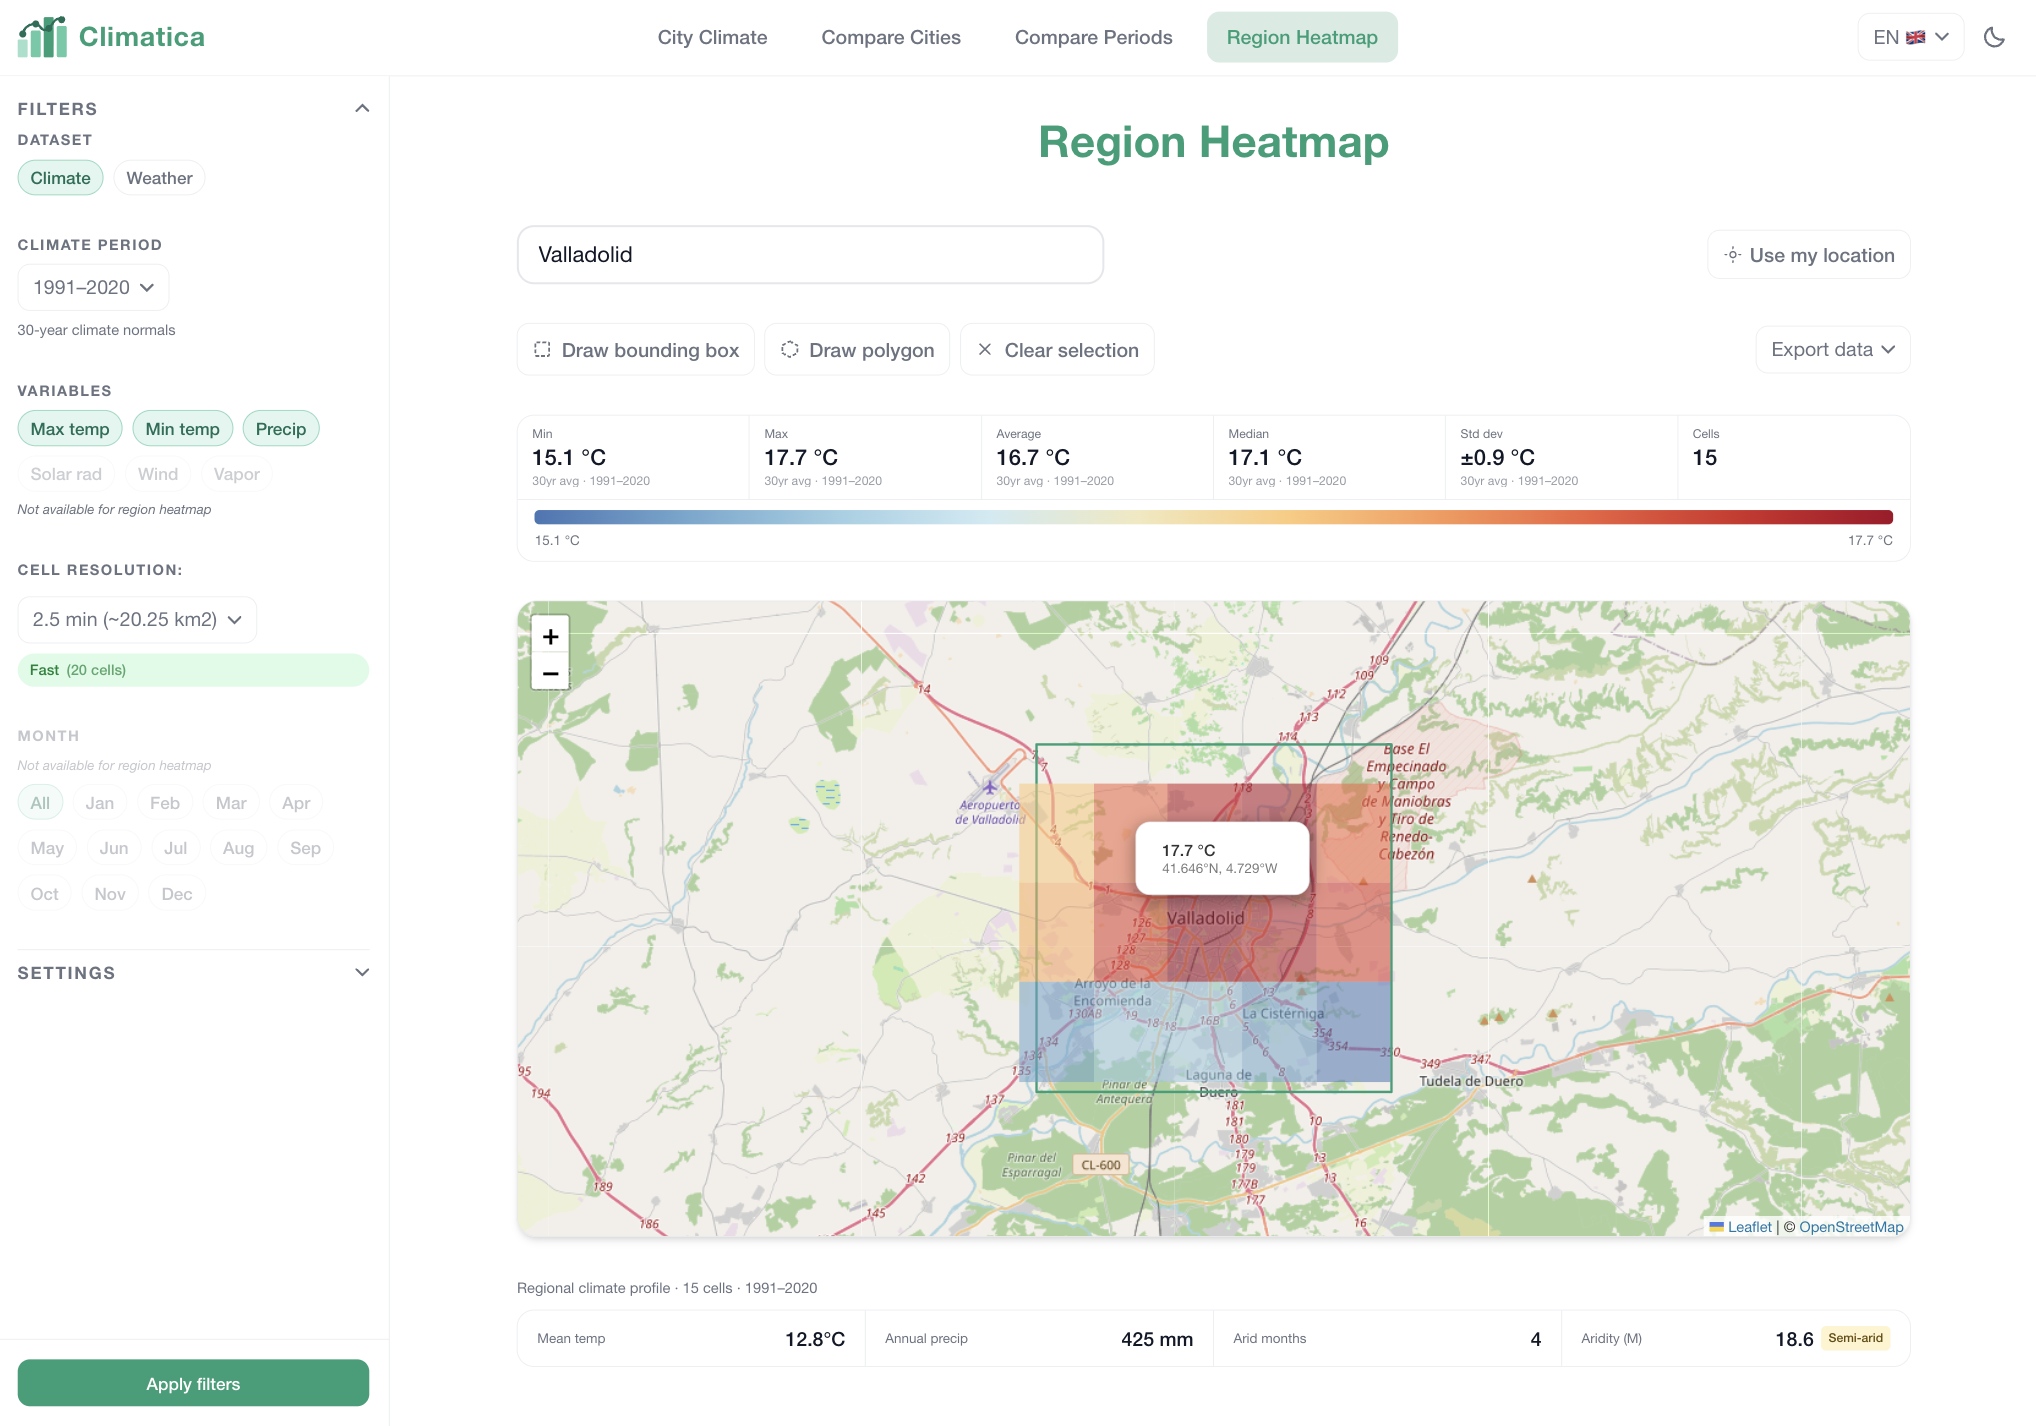
\includegraphics[width=0.9\textwidth]{Images/climatica-demo-fmp-heatmap.png}
  \caption{Region Heatmap page showing the spatial distribution of annual
    average maximum temperature around Valladolid (climate dataset,
    1991--2020). The urban core reaches 17.7\,$^\circ$C while peripheral
    cells are as cool as 15.1\,$^\circ$C. The regional profile below the
    map summarises the 15 queried cells.}
  \label{fig:demo_fmp_heatmap}
\end{figure}

\subsubsection{Step 4: Comparing Alternative Sites}

As a final step, the manager uses the \textbf{Compare Cities} page to place
Valladolid alongside \textbf{Salamanca}, a city 120\,km to the southwest
(Figure~\ref{fig:demo_fmp_cities}). The side-by-side comparison under the
1991--2020 normal shows that Salamanca is already warmer (+1.1\,$^\circ$C
average maximum) and slightly drier (419\,mm vs.\ 420\,mm), with both cities
sharing five arid months and a Martonne index in the Semi-arid range
(16.8 vs.\ 18.1). The insight cards at the bottom confirm that Salamanca is
the warmer city by 1.2\,$^\circ$C. The manager uses this comparison to inform
a precautionary approach: species that are currently performing well in
Salamanca's stands under equivalent soil conditions (\textit{Quercus suber},
\textit{Pinus pinaster}) are candidates for introduction into the Valladolid
management unit as climate analogues for mid-century conditions.

\begin{figure}[H]
  \centering
  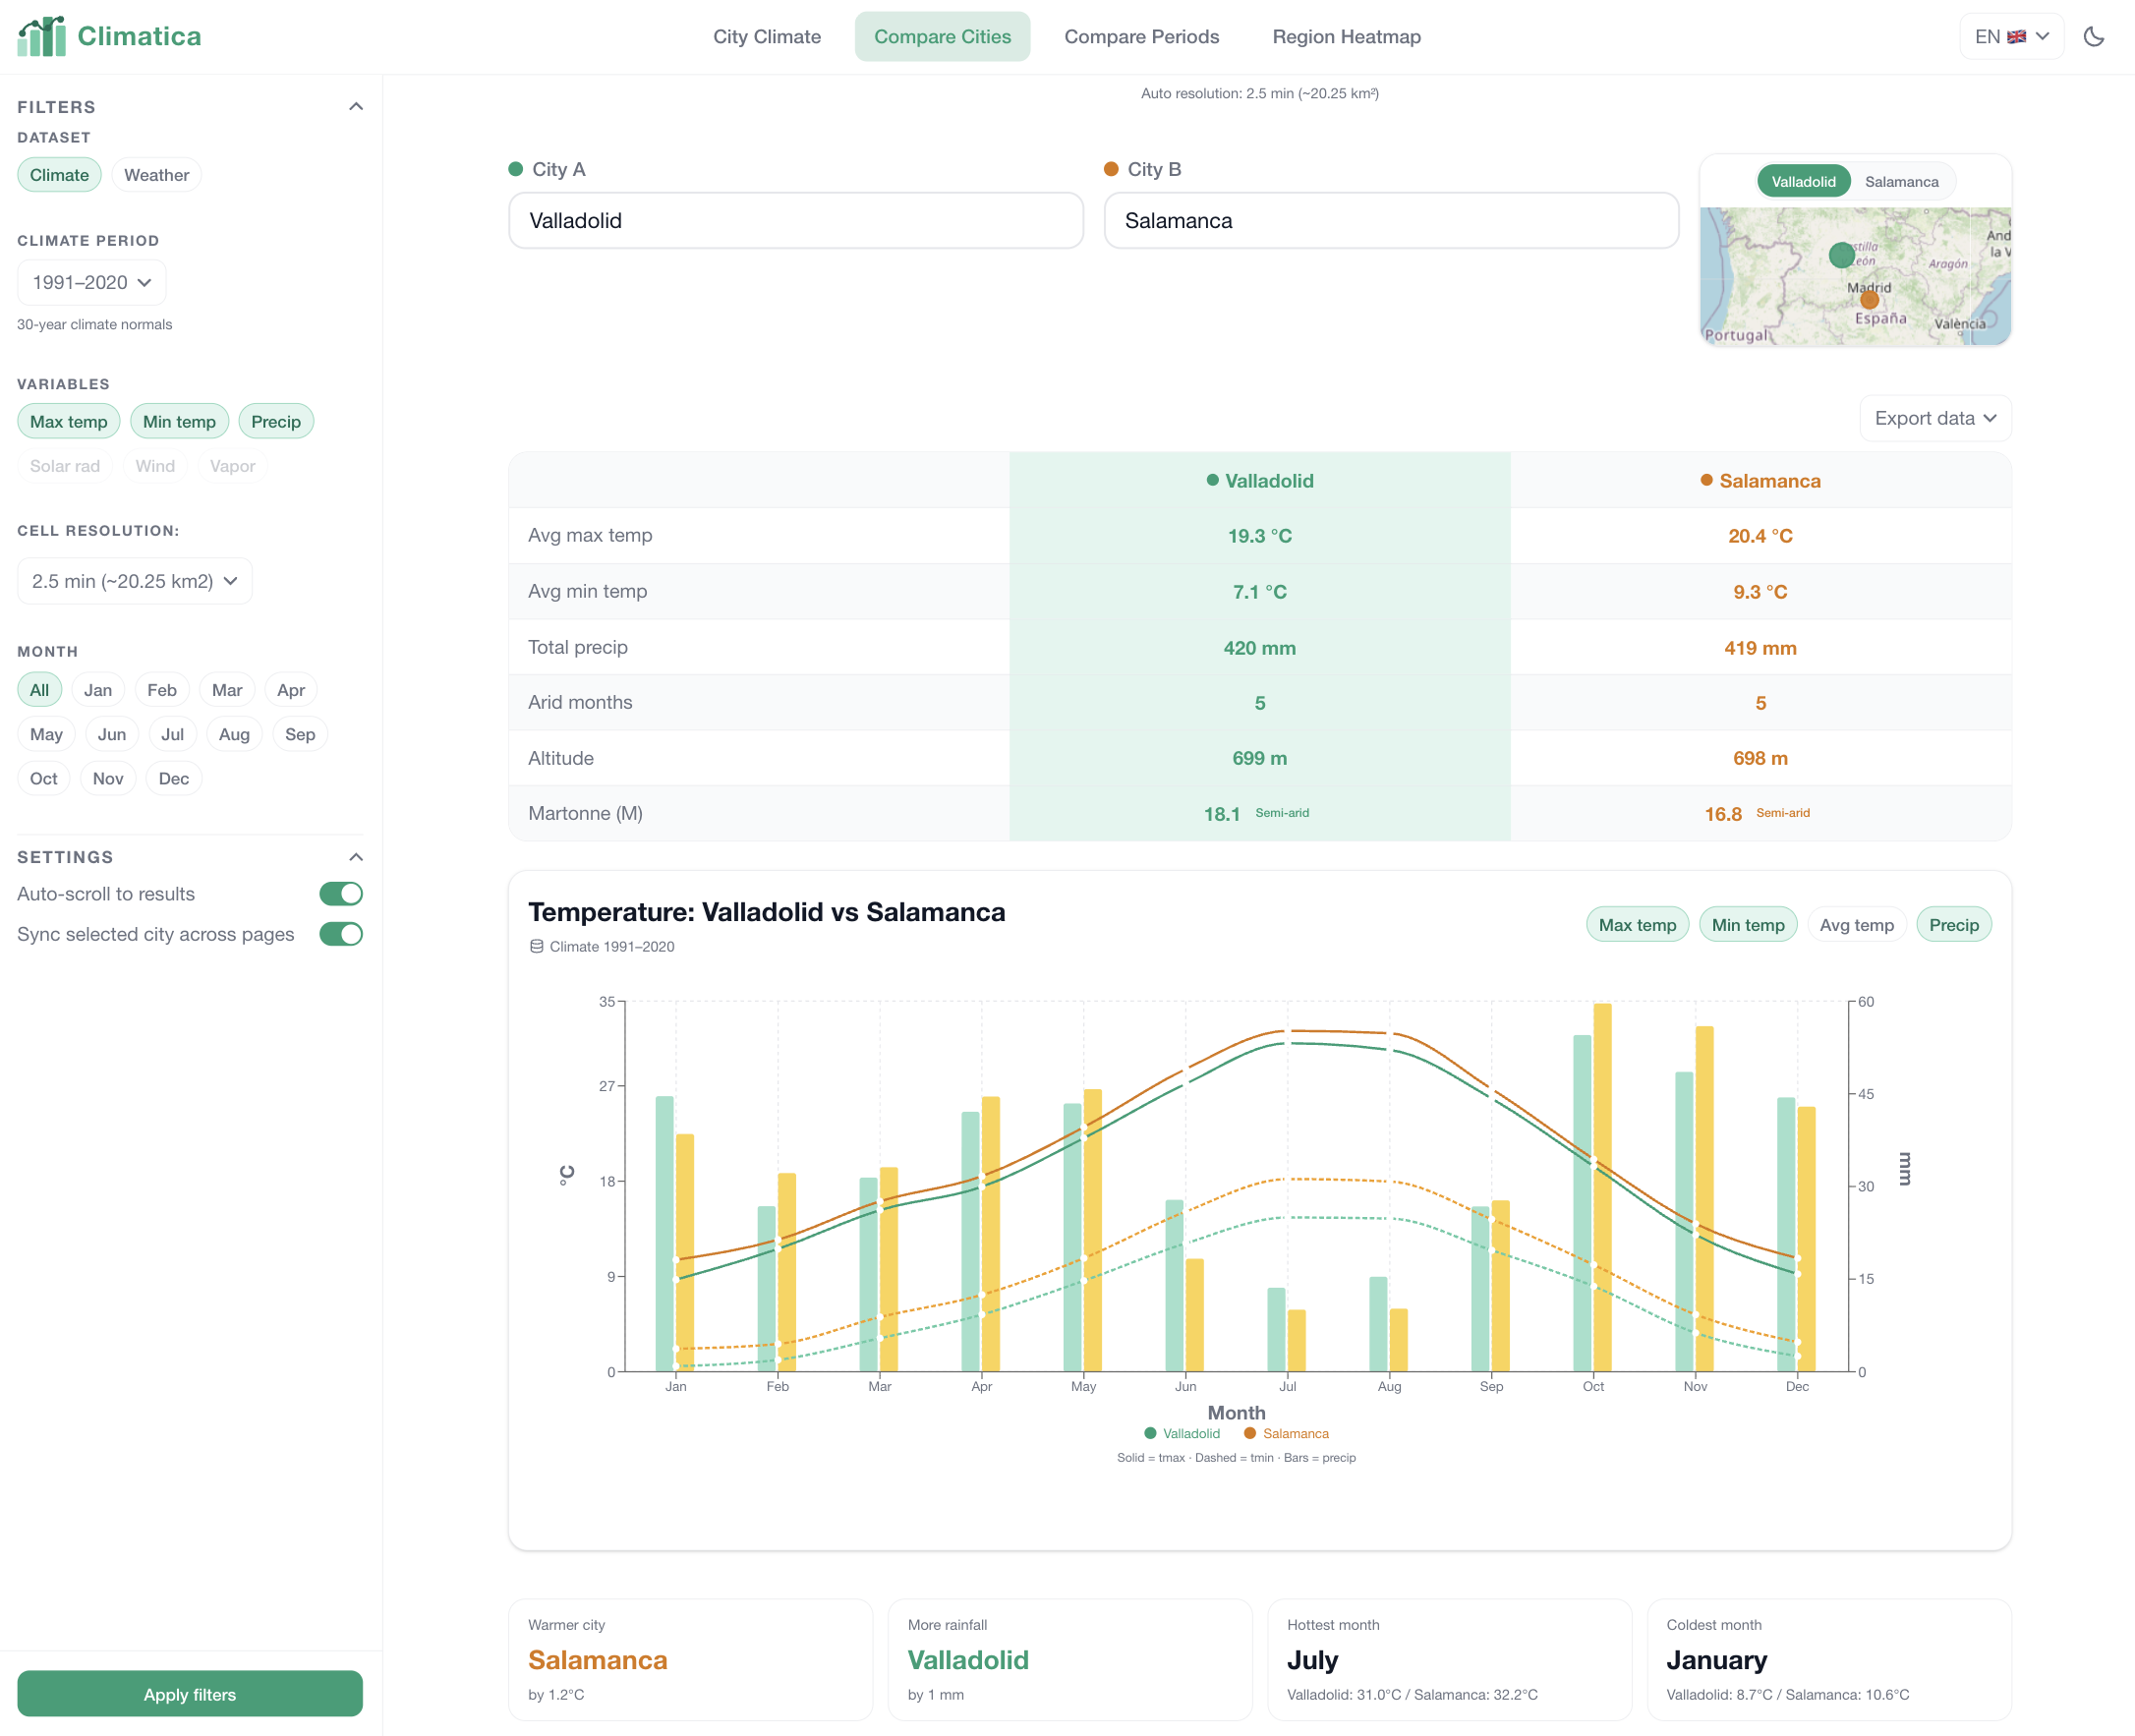
\includegraphics[width=0.9\textwidth]{Images/climatica-demo-fmp-compare-cities.png}
  \caption{Compare Cities page placing Valladolid (green) alongside Salamanca
    (orange) under the 1991--2020 climate normal. Salamanca's higher average
    maximum temperature (20.4\,$^\circ$C vs.\ 19.3\,$^\circ$C) and lower
    Martonne index (16.8 vs.\ 18.1) make it a useful climate analogue for
    the conditions Valladolid may face in coming decades.}
  \label{fig:demo_fmp_cities}
\end{figure}

\subsubsection{Outcome}

In under fifteen minutes and without installing any software or writing any
code, the forest manager has: (1)~established the current climate baseline for
the site under the most recent 30-year normal; (2)~quantified the observed
shift over the past 60 years (+1.0\,$^\circ$C, $-$12\,mm, one additional arid
month); (3)~mapped the spatial variation in temperature across the management
unit at 2.5-minute resolution; and (4)~identified a nearby analogue site to
guide species selection under anticipated future conditions. All four pages of
Climatica contributed directly to this workflow, and the results are grounded
in the same WorldClim raster archive that would underpin a formal scientific
assessment.

% ─── 4.5.2 Scenario 2 ────────────────────────────────────────────────────────
\subsection{Scenario 2: Detecting Climate-Driven Forest Stress}\label{EVAL_DEMO_DECLINE}

\subsubsection{Context}

Climate change is increasingly recognised as a primary driver of forest decline
across Europe and North America. Warmer temperatures and prolonged summer
droughts weaken the physiological defences of trees, making them susceptible
to secondary agents --- most notably bark beetle outbreaks, which have caused
catastrophic mortality in spruce and pine stands across Central Europe and
Scandinavia over the past two decades~\cite{seidl2017bark}. Understanding
whether a particular site has experienced a meaningful shift towards warmer or
drier conditions over the period in which decline has been observed is a
necessary first step in attributing mortality to climate stress rather than to
other causes such as competition, soil degradation, or pathogen pressure.

An ecologist investigating pine stands in the western Pyrenees that have shown
elevated mortality and bark beetle damage since approximately 2010 wants to
establish whether the local climate has shifted meaningfully over the study
period. The nearest city representative of the study area is \textbf{Pamplona}
(Navarra, Spain).

\subsubsection{Step 1: Multi-period Temperature Trend}

The ecologist opens the \textbf{Compare Periods} page, selects Pamplona, and
switches to Weather mode. Using the multi-year selector in the sidebar, five
years are chosen to span the full observation window: 1985, 1995, 2005, 2015,
and 2023. Each year is assigned a distinct colour (green, amber, blue, rose,
violet) and the overlaid chart renders all five maximum temperature curves
simultaneously (Figure~\ref{fig:demo_decline_multiyear}).

The statistics table reveals a clear warming signal: average annual maximum
temperature increased from 17.7\,$^\circ$C in 1985 to 19.6\,$^\circ$C in
2023 --- a rise of \textbf{+1.9\,$^\circ$C} over 38 years. The year 2015
stands out with the highest average maximum temperature (18.7\,$^\circ$C),
consistent with the record European heat conditions of that year. The tooltip
on the July peak confirms that July maximum temperatures were 27\,$^\circ$C
in 1985--2005 and rose to 28--29\,$^\circ$C in 2015--2023.

\begin{figure}[H]
  \centering
  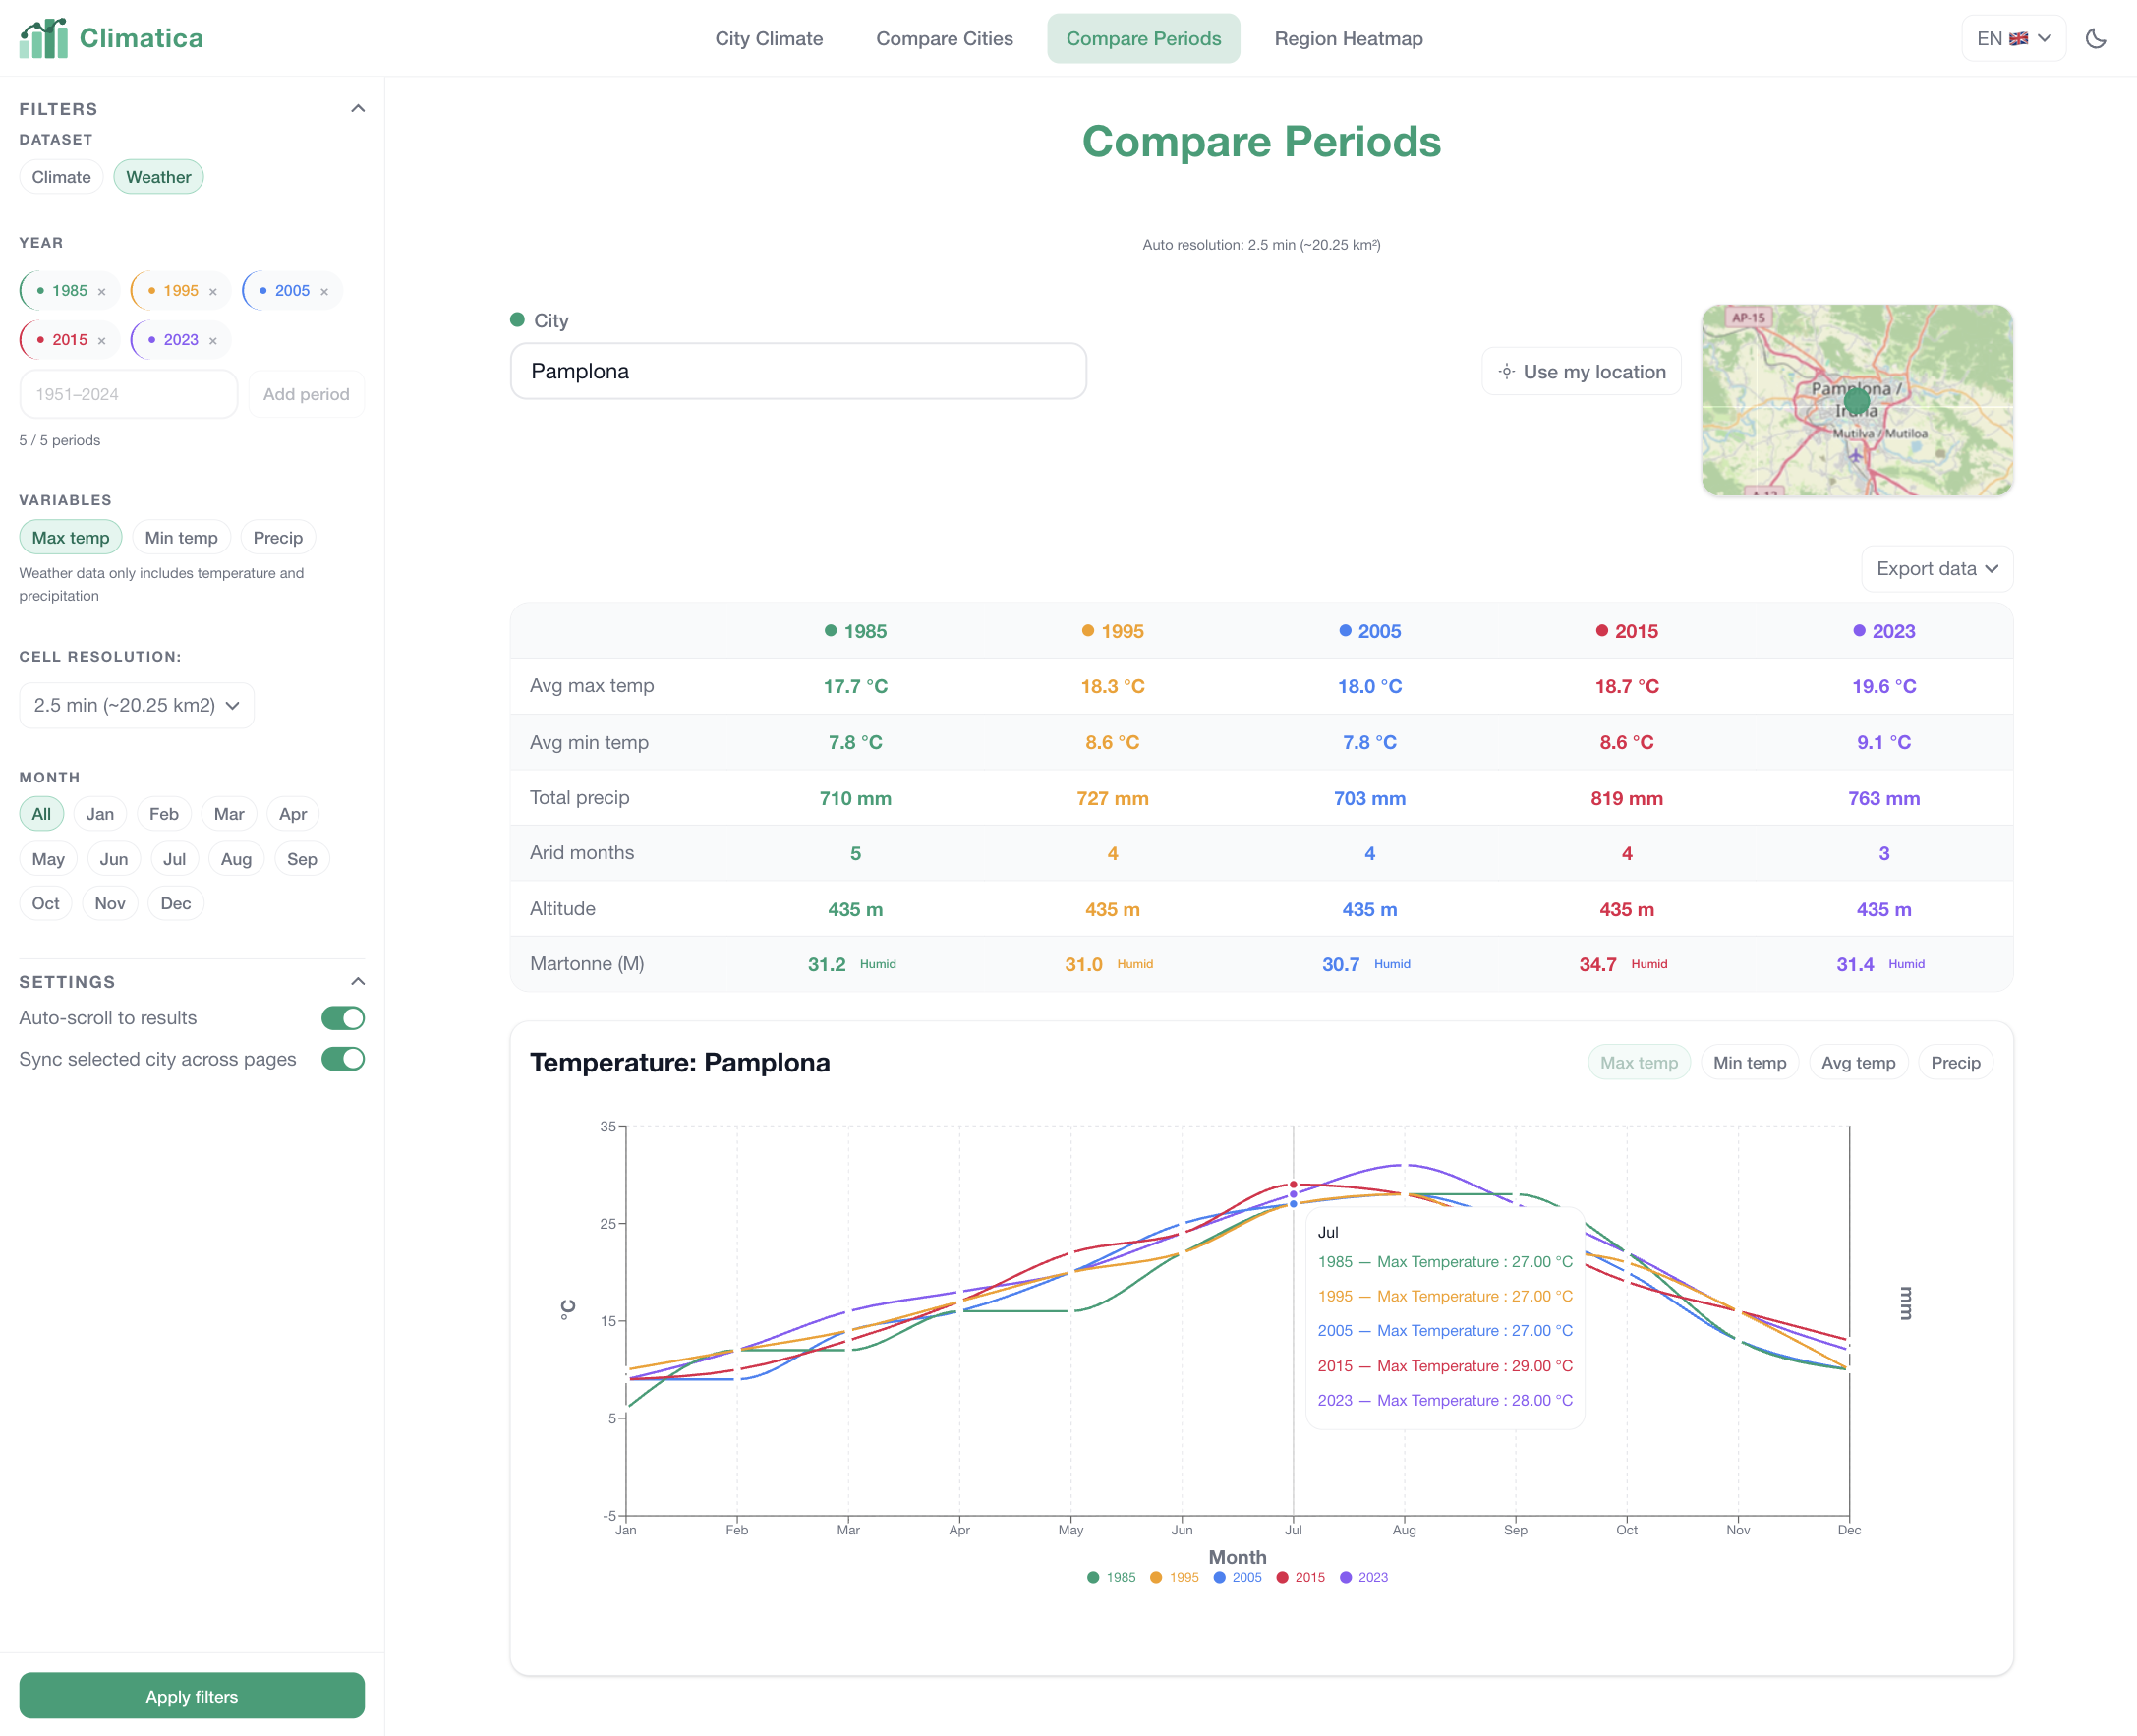
\includegraphics[width=0.9\textwidth]{Images/climatica-demo-decline-multiyear.png}
  \caption{Compare Periods page in weather mode for Pamplona showing five
    selected years (1985, 1995, 2005, 2015, 2023) with maximum temperature.
    The statistics table shows average annual maximum temperature rising from
    17.7\,$^\circ$C in 1985 to 19.6\,$^\circ$C in 2023 (+1.9\,$^\circ$C).
    The tooltip confirms July maximum temperatures of 27\,$^\circ$C in the
    earlier years versus 28--29\,$^\circ$C in recent years.}
  \label{fig:demo_decline_multiyear}
\end{figure}

\subsubsection{Step 2: Precipitation and Aridity Trend}

The ecologist switches the chart variable to \textbf{Precipitation}
(Figure~\ref{fig:demo_decline_precip}). The picture here is more variable:
total annual precipitation ranges from 703\,mm (2005) to 819\,mm (2015),
with no clear monotonic trend. However, the Martonne aridity index in the
statistics table shows that all five years remain in the \emph{Humid} category
(M~$>$~30), with values between 30.7 and 34.7. The bar chart reveals that
inter-annual variability in summer precipitation is high, with some years
showing near-zero July and August precipitation while others show moderate
values. The combination of rising maximum temperatures and variable but
occasionally very dry summers creates the drought stress conditions most
damaging to \textit{Pinus sylvestris}.

\begin{figure}[H]
  \centering
  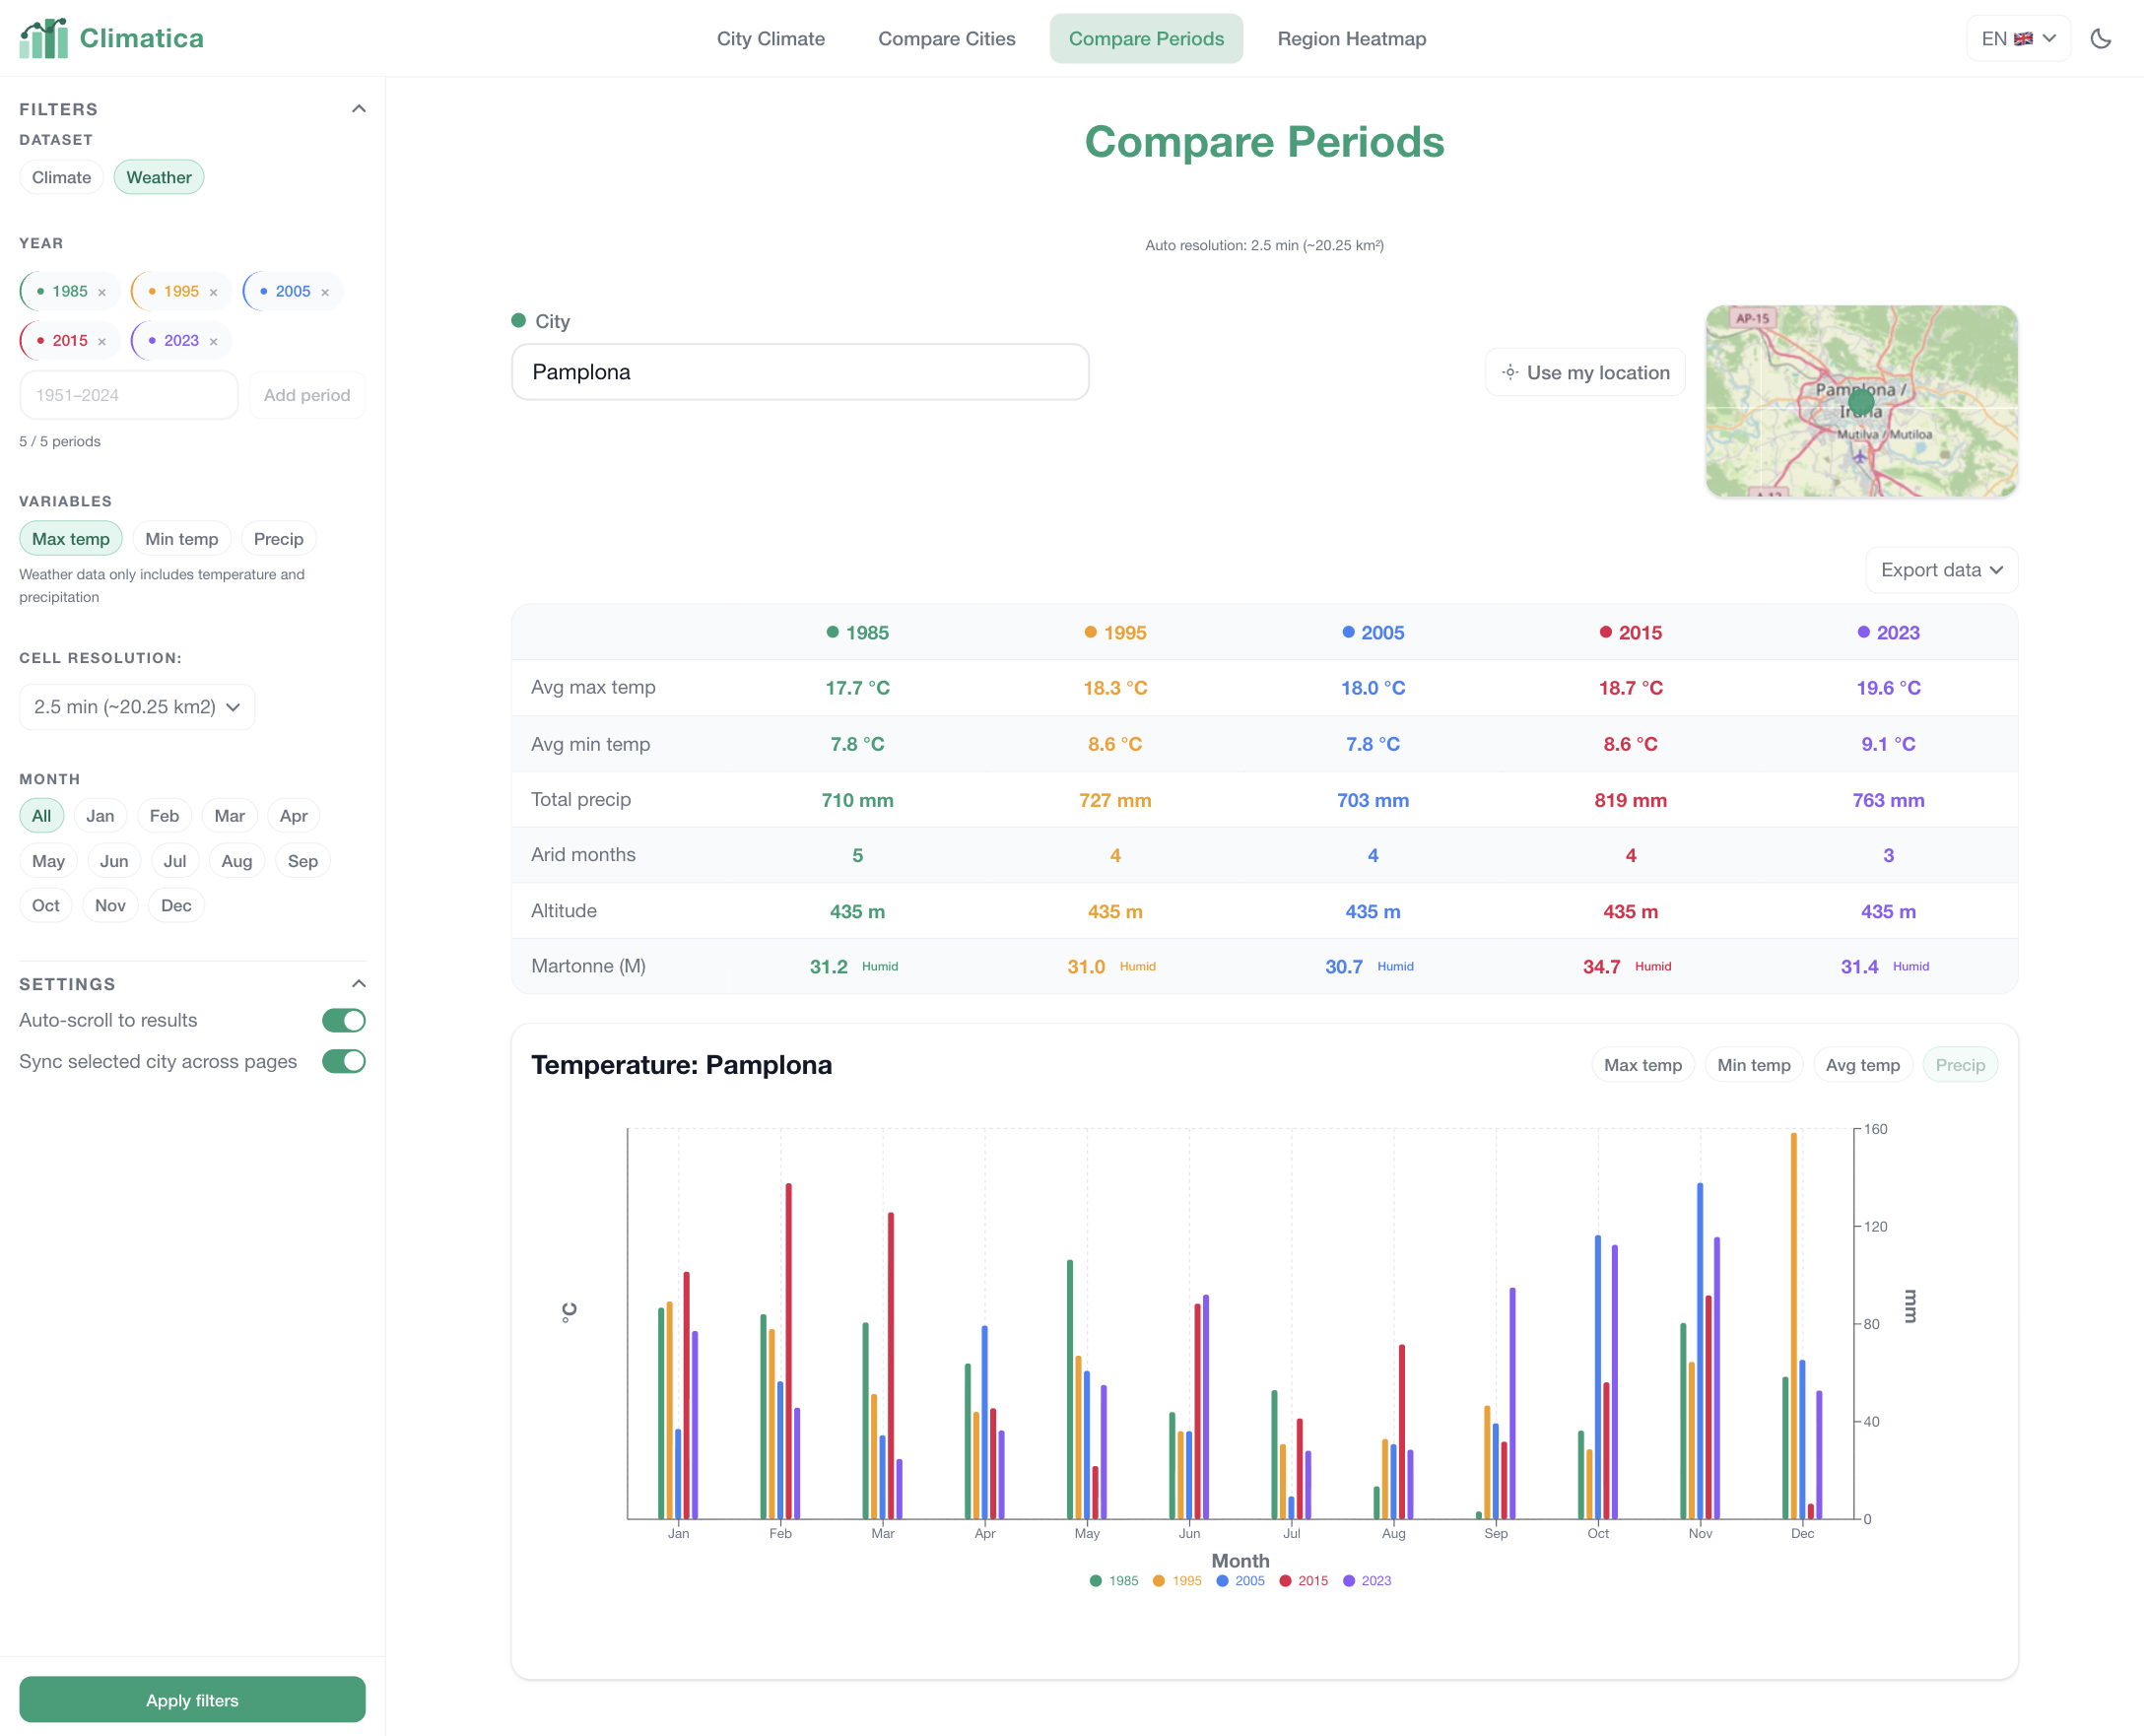
\includegraphics[width=0.9\textwidth]{Images/climatica-demo-decline-precipitation.png}
  \caption{Compare Periods page in weather mode for Pamplona with precipitation
    selected. The bar chart shows high inter-annual variability in summer
    precipitation across the five years. The Martonne index (30.7--34.7)
    keeps all years in the Humid category, but the combination of rising
    temperatures and occasional summer drought creates physiological stress
    conditions for conifers.}
  \label{fig:demo_decline_precip}
\end{figure}

\subsubsection{Step 3: Spatial Extent of the Stress Signal}

To assess whether the stress conditions are localised or part of a broader
regional pattern, the ecologist switches to the \textbf{Region Heatmap} page
and draws a polygon around the Pyrenean foothills east of Pamplona
(Figure~\ref{fig:demo_decline_heatmap}). Using the weather dataset for 1991,
the heatmap over 34 cells reveals a strong elevation-driven thermal gradient:
the lowland cells in the Ebro valley to the south reach annual average maximum
temperatures above 11\,$^\circ$C, while the higher-elevation cells in the
Pyrenean ranges to the north are distinctly cooler (down to 6.8\,$^\circ$C).
The regional profile confirms a mean temperature of 11.0\,$^\circ$C, annual
precipitation of 918\,mm, and a Martonne index of 43.8 (\emph{Very-humid}) ---
conditions that support dense conifer forest but that are increasingly
susceptible to drought stress during anomalously dry summers.

The spatial pattern makes clear that the bark beetle risk is not uniform across
the landscape: the warmer, south-facing lowland cells are under greater thermal
stress than the cooler highland cells, and any management intervention aimed
at reducing stand vulnerability should prioritise the lower-elevation zones.

\begin{figure}[H]
  \centering
  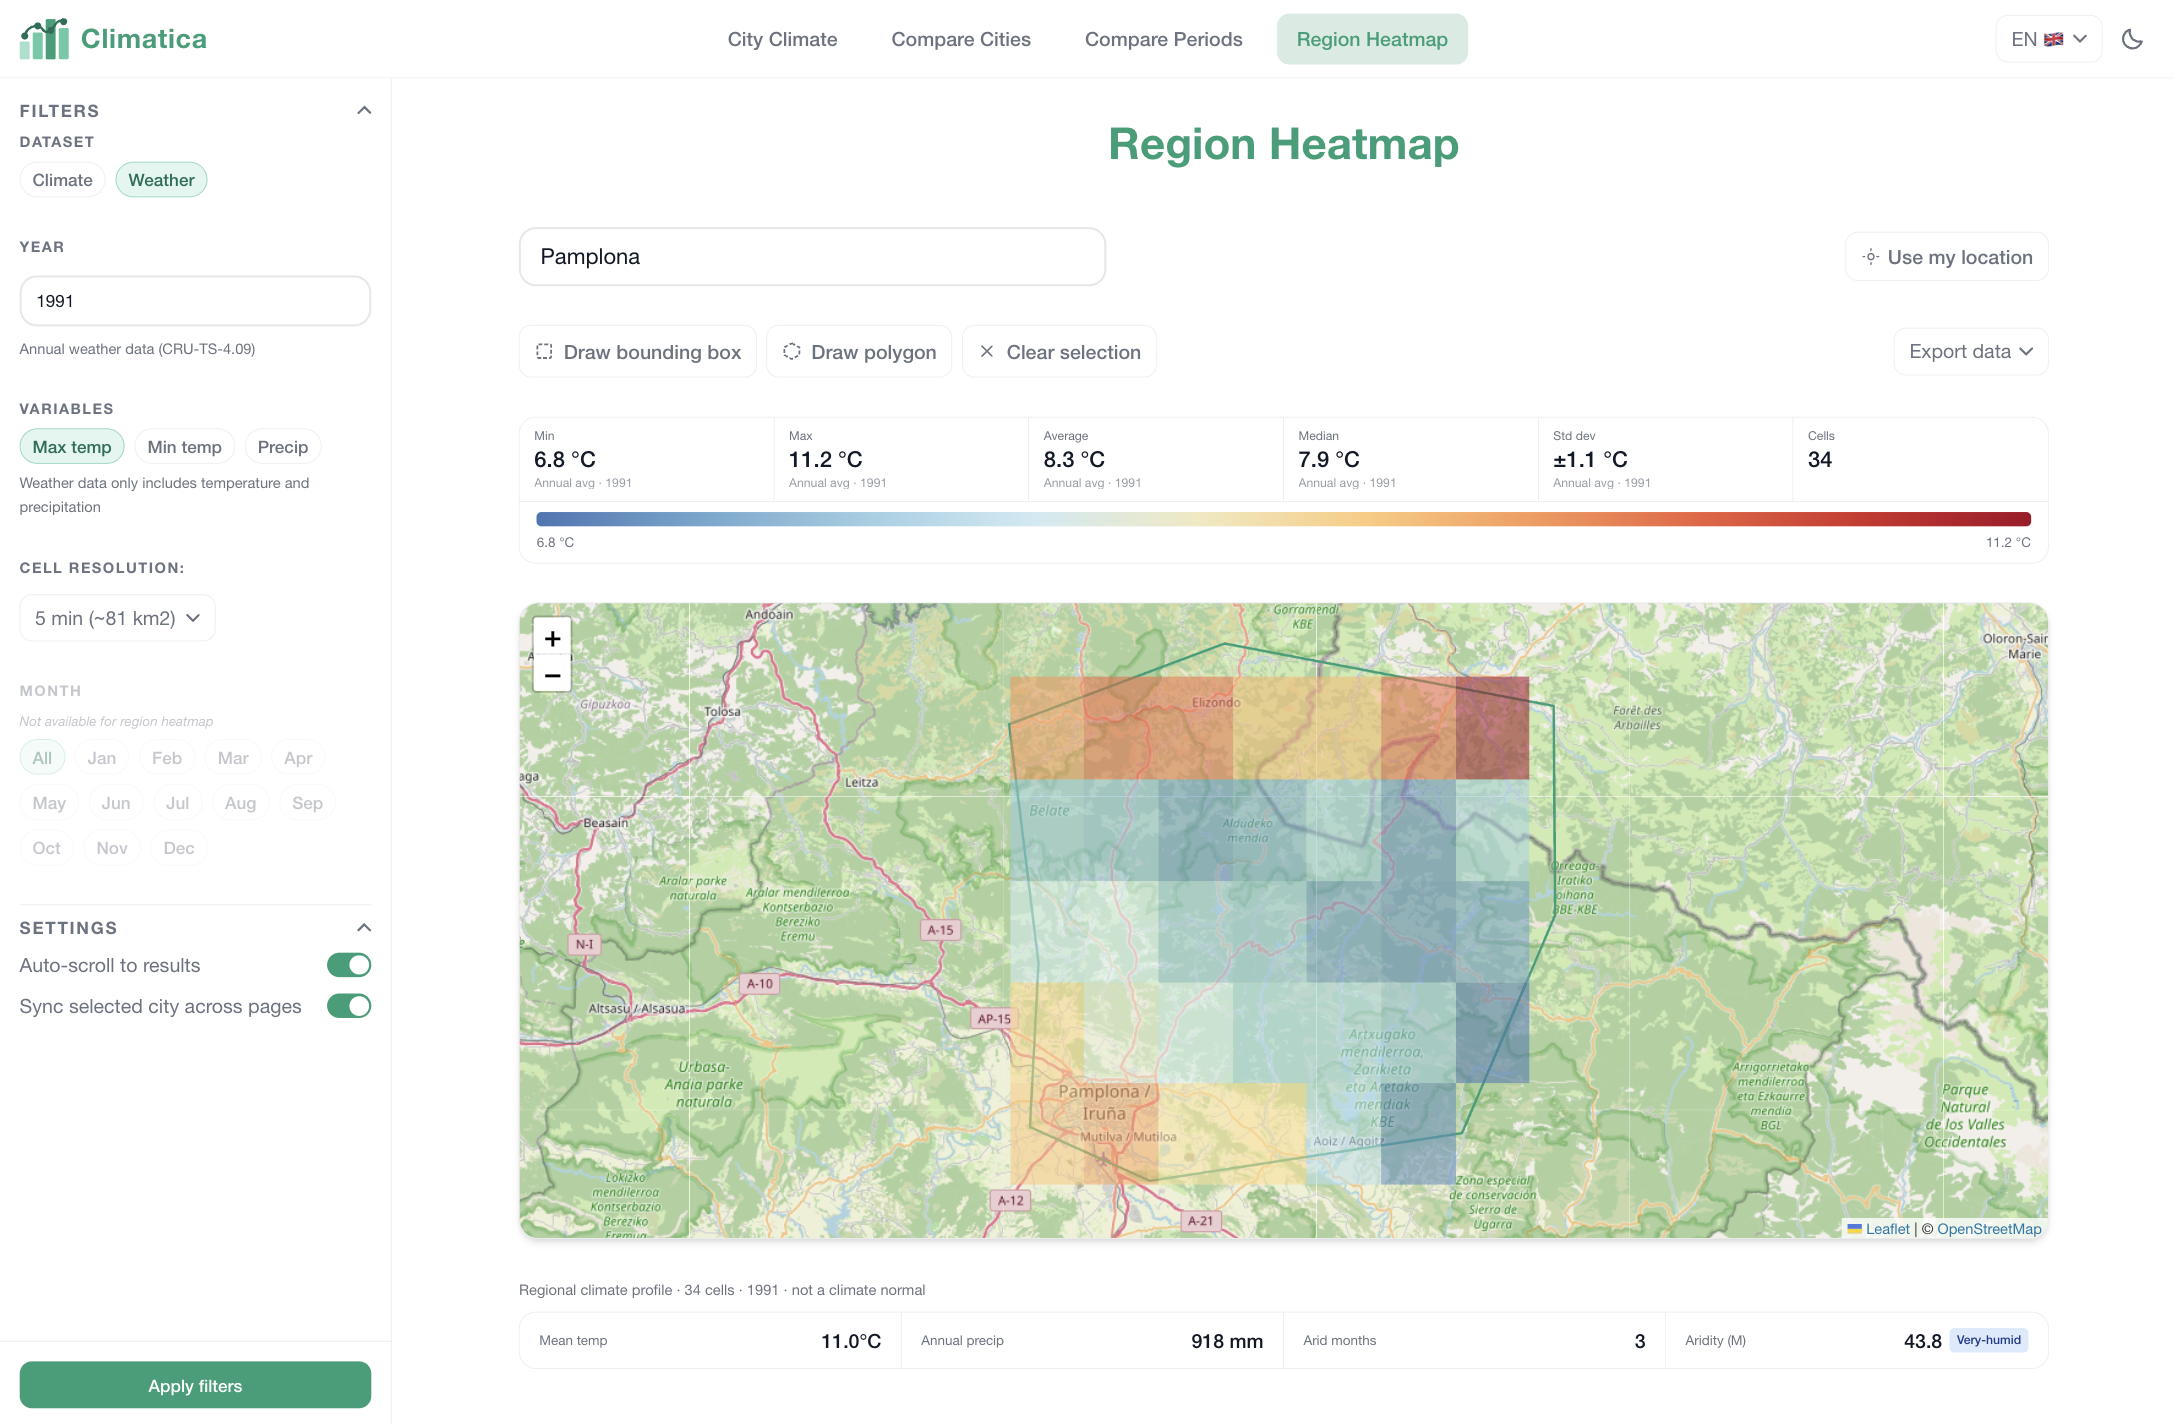
\includegraphics[width=0.9\textwidth]{Images/climatica-demo-decline-heatmap.png}
  \caption{Region Heatmap page showing annual average maximum temperature
    across the Pyrenean foothills east of Pamplona (weather dataset, 1991).
    The thermal gradient from the warm Ebro valley lowlands (orange--red cells,
    $>$\,11\,$^\circ$C) to the cooler Pyrenean highlands (blue cells,
    $<$\,7\,$^\circ$C) is clearly resolved across 34 cells. The regional
    profile confirms a mean temperature of 11.0\,$^\circ$C and annual
    precipitation of 918\,mm (Martonne index 43.8, Very-humid).}
  \label{fig:demo_decline_heatmap}
\end{figure}

\subsubsection{Outcome}

Within a single session, the ecologist has assembled a coherent body of
evidence linking the observed forest decline to a documented multi-decade
warming trend at the study site (+1.9\,$^\circ$C over 38 years), high
inter-annual variability in summer precipitation creating periodic drought
stress, and a spatially resolved thermal gradient that identifies the
lower-elevation, south-facing zones as the most vulnerable parts of the
landscape. This evidence base --- which would previously have required manual
extraction from WorldClim GeoTIFF files and custom scripting --- was assembled
interactively in approximately twenty minutes, using only a web browser and
no specialist software.

% ─── 4.6 Discussion ──────────────────────────────────────────────────────────
\section{Discussion}\label{EVAL_DISCUSS}

\subsection{Interpretation of Results}\label{EVAL_DISCUSS_RESULTS}

The quantitative results are encouraging. A mean SUS score of 84.6 places
Climatica in the \emph{Excellent} range on the Bangor et al.\ adjective scale,
well above the industry average of 68. The NPS of +44 indicates that a
substantial majority of participants would recommend the tool to peers. Both
metrics suggest that Climatica successfully delivers on its primary design goal
of being accessible to non-specialist users without requiring GIS or programming
expertise.

The qualitative feedback reinforces this conclusion. The dominant theme in the
``liked most'' responses was ease of use, which was mentioned unprompted by
approximately 80\% of respondents. This is particularly meaningful given that
the participant group had intermediate knowledge of climatology and GIS but
limited programming and database backgrounds --- precisely the audience for
whom the application was designed. The contrast with the tools surveyed in
Chapter~\ref{REL} is evident: platforms such as NASA Giovanni and Copernicus
C3S offer greater scientific depth, but their learning curve excludes the kind
of users who found Climatica immediately accessible.

The three lowest SUS scores (47.5, 50.0, and 65.0) merit attention. Examining
the corresponding qualitative responses reveals different explanations. One
respondent with a low score reported finding parts of the navigation
``confusing'' and requested tutorials, suggesting a genuine discoverability
issue. A second reported slow loading and the heatmap stopping after the first
query, which points to a performance and state-management bug rather than a
design problem. The third low score came from a respondent who gave uniformly
low ratings without elaboration in the free-text fields, making the root cause
unclear.

\subsection{Limitations}\label{EVAL_DISCUSS_LIMITS}

Several limitations of this evaluation should be noted.

\textbf{Sample size and representativeness.} Twenty-seven respondents is a
reasonable number for a SUS study --- Tullis and Stetson~\cite{tullis2004sus}
showed that reliable SUS estimates can be obtained with as few as 12--14
participants --- but the sample was drawn from a single presentation event,
which limits its diversity. All participants were European university students
in natural science programmes; the results may not generalise to other user
groups such as secondary school students, urban planners, or researchers in
data-sparse regions.

\textbf{Evaluation duration.} Participants used the application for
approximately ten minutes before completing the questionnaire. Short exposure
times are standard in SUS studies but may not reveal usability issues that
only emerge with sustained use, such as the filter workflow friction reported
by some respondents.

\textbf{Device and browser variability.} The PNG export alignment issue was
reported by multiple respondents using different devices. The evaluation did
not systematically record device and browser information, so it is not possible
to determine whether the issue affected all platforms equally or was
concentrated in specific configurations.

\textbf{Data accuracy concerns.} Two respondents noted that the altitude
displayed for their city did not match their expectations, even at the highest
resolution. This is an inherent limitation of the WorldClim interpolation
methodology (described in Section~\ref{REL_WORLDCLIM_INTERP}): elevation values
are derived from a digital elevation model, and the 900\,m cell size of the
30-second grid means that local topographic variation within a cell is not
captured. This limitation is shared by all tools built on WorldClim data.

\subsection{Future Work}\label{EVAL_DISCUSS_FUTURE}

The evaluation results point to several concrete directions for future
development.

\textbf{Export improvements.} Fixing the PNG alignment issue and ensuring
consistent SVG export across platforms and browsers are the highest-priority
items based on frequency of mention. Adding a raw data download option --- a
CSV or JSON export of the full monthly pixel values --- would address the most
technically sophisticated user requests.

\textbf{Filter workflow.} Making filter changes take effect immediately,
without requiring an explicit ``Apply'' click, would satisfy the most commonly
raised workflow complaint. This would require redesigning the draft filter
pattern to debounce API calls rather than gate them behind a button.

\textbf{Additional climate periods.} Supporting 10-year normals and
non-overlapping period ranges would significantly expand the temporal analysis
capability. These features are technically feasible given the SCRAPI data model,
which exposes individual weather years from 1951 to 2024.

\textbf{Heatmap performance.} Rendering thousands of \texttt{L.rectangle}
overlays is the primary bottleneck for large bounding boxes at fine resolution.
Migrating the heatmap renderer to a WebGL-backed layer (e.g.\ using
\texttt{leaflet.heat} or a custom Canvas layer) would provide an order-of-magnitude
performance improvement for large queries.

\textbf{Mobile support.} One respondent requested a mobile application;
another noted that PNG exports were misaligned on iPad. The current Next.js
deployment serves a responsive web interface, but the map drawing interactions
(bounding box and polygon) are not yet optimised for touch input.

\textbf{Extended language support.} Adding further locales beyond English,
Spanish, and Ukrainian would broaden accessibility. The \texttt{next-intl}
infrastructure already in place makes adding new locales straightforward;
the main effort is in translating the 233 keys per locale.










% ─── CHAPTER 5 ────────────────────────────────────────────────────────────────
\chapter{Conclusions and Future Work}\label{CONC}
% TODO

% ─── BIBLIOGRAPHY ─────────────────────────────────────────────────────────────
\printbibliography[title=References]
\addcontentsline{toc}{chapter}{References}

\end{document}